\documentclass{beamer}

\usepackage[ngerman]{babel}
\usepackage[utf8]{inputenc}
\usepackage[T1]{fontenc}
\usepackage{lmodern}

\usepackage[german,linesnumbered,algoruled,longend,vlined]{algorithm2e}
\DontPrintSemicolon
\SetArgSty{}
\SetKw{KwOr}{or}
\SetKw{KwAnd}{and}
\SetKw{KwNot}{not}
\setlength{\algomargin}{3ex}

\usepackage[fixlanguage]{babelbib}
% \selectlanguage{ngerman}
\setbibliographyfont{title}{}
\setbibliographyfont{jtitle}{}
\setbibliographyfont{btitle}{\emph}
\setbibliographyfont{stitle}{\emph}
\setbibliographyfont{journal}{\emph}

\usepackage{amsmath}
\usepackage{amsfonts}
\usepackage{amssymb}
\usepackage{amsthm}

\usepackage{graphicx}
\usepackage{enumerate}
\usepackage{textcomp}
\usepackage{epstopdf}

%\newtheorem{satz}{Satz}[chapter]
%\newtheorem{lemma}[satz]{Lemma}
%\newtheorem{beobachtung}[satz]{Beobachtung}
%\newtheorem{folgerung}[satz]{Folgerung}
%\newtheorem{korollar}[satz]{Korollar}
%\theoremstyle{definition}
%\newtheorem{definition}[satz]{Definition}
%\newenvironment{beweis}{\begin{proof}}{\end{proof}}

\graphicspath{{abbildungen/}}

% Eigene Commands:
\newcommand{\Epsilon}{\mathcal{E}}
\newcommand{\N}{\mathbb{N}}
%\newtheorem{example}[satz]{Beispiel}

\hyphenation{Teil-as-pekt Teil-as-pek-te}

\begin{document}
%%%%%%%%%%%%%%%%%%%%%%%%%%%%%%%%%%%%%%%%%%%%%%%%%%%%%%%%%%%%%%%%%%%%%%%%%%
%%%%%%%%%%%%% Bitte nur ab hier Änderungen vornehmen %%%%%%%%%%%%%%%%%%%%%

%% hier Titel und Autorennamen eintragen

\subject{Bachelorarbeit}
\title{Implementierung eines Algorithmus\\ für das glatt"=orthogonale Zeichnen \\ planarer Graphen} % Geben Sie hier den Titel Ihrer Arbeit an.
\author{Bernhard Häussner} % Geben Sie Ihren Namen an. 
\date{Bachelor-Kolloquium am 12. Mai 2014} % TODO: Geben Sie das Abgabedatum an, entfernen Sie das Versionsdatum ( \\ Version \today)
\institute{Julius-Maximilians-Universität Würzburg\\
Institut für Informatik\\
Lehrstuhl für Informatik I\\
Effiziente Algorithmen und wissensbasierte Systeme\\[\baselineskip]
Betreuer:\\
Prof.\ Dr.\ Alexander Wolff\\
Dipl.-Inf.\ Philipp Kindermann} % Geben Sie den Namen des weiteren Betreuers an
\maketitle


\section{Einleitung}

\begin{frame}
  \frametitle{Implementierung eines Algorithmus für das glatt"=orthogonale Zeichnen planarer Graphen}
  \begin{itemize}[<+->]
    \item Zeichnen von Graphen: Knoten platzieren, Kanten zeichnen
    \item glatt"=orthogonal: besonders übersichtlich
    \item Planarität: Keine Überschneidungen von Kanten
    \item Algorithmus: Alam et al.~\cite{smooth-13}
    \item Implementierung: Test mit vielen Graphen
  \end{itemize}
\end{frame}

\begin{frame}
  \frametitle{Ein Liniennetzplan}
  \begin{figure}[h]
    \centering
    \fbox{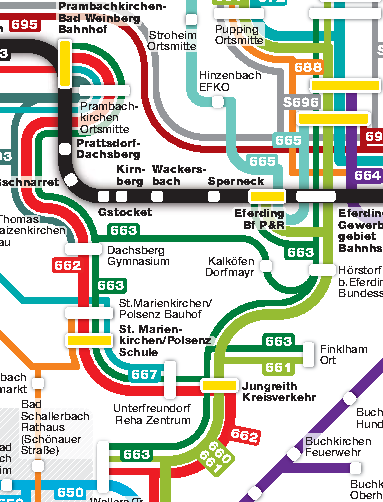
\includegraphics[height=5cm]{liniennetzplan}}
    \caption{Ein Ausschnitt aus dem Liniennetzplan \emph{Eferding -- Grieskirchen -- Wels}, Helge Waldherr, 2014. \footnotesize{\url{http://www.ooevv.at/upload/content/blaetterkatalog/Liniennetzplan/EF-GR-WE/assets/common/downloads/Liniennetzplan-GR-EF.pdf}}}
    \label{fig:liniennetzplan}
  \end{figure}
\end{frame}

\begin{frame}
  \frametitle{Vom Liniennetzplan zur glatt-orthogonalen planaren Zeichnung}
  \begin{itemize}[<+->]
    \item Liniennetzpläne für jedermann ohne Vorwissen benutzbar
    \item Abstraktion: Haltestellen $\mapsto$ Knoten, Strecken $\mapsto$ Kanten
    \item Reduktion: Keine Beschriftungen, Überschneidungen oder parallele Strecken
    \item Ziel: Platzierung der Knoten, rundes zeichnen der Kanten
    \item Überschneidungen der glatt-orthogonalen Kanten vs. Komplexität
  \end{itemize}
\end{frame}

% go/zeichnung

\section{Grundlegendes}
\frame{\tableofcontents[currentsection]}

\begin{frame}
  \frametitle{Graphen}
  \begin{itemize}[<+->]
    \item Tupel $G = (V, E)$ von Mengen, wobei $E \subset \mathcal{P}(V)$
    \item Ungerichtete Graphen
    \item Einfache Graphen
    \item Zusammenhängende Graphen
    \item Bsp: $G_\text{E} = (V_\text{E}, E_\text{E})$; $V_\text{E} = \{0, 1, 2, 3, 4\}$; $E_\text{E} = \{\{0, 1\}, \{0, 2\}, \{0, 4\}, \{1, 2\}, \{1, 4\}, \{2, 3\}, \{2, 4\}, \{3, 4\}\}$

  \end{itemize}
\end{frame}


\begin{frame}
  \frametitle{Planare Einbettung}

\begin{columns}[c]
\begin{column}{5cm}
  \begin{itemize}[<+->]
    \item Planarer Graph: kann ohne Überschneidungen gezeichnet werden
    \item Kanten können sich an den Knoten berühren
    \item Zeichnen mit planarer Einbettung durch Reihenfolge der Kanten in Adjazenzliste
    \item Berechnen mit Algorithmus von Brandes~\cite{brandes-09}
    \item Ausführlicher Pseudocode, leicht zu implementieren

  \end{itemize}
\end{column}
\begin{column}{5cm}
        \begin{figure}[h]
                \centering
                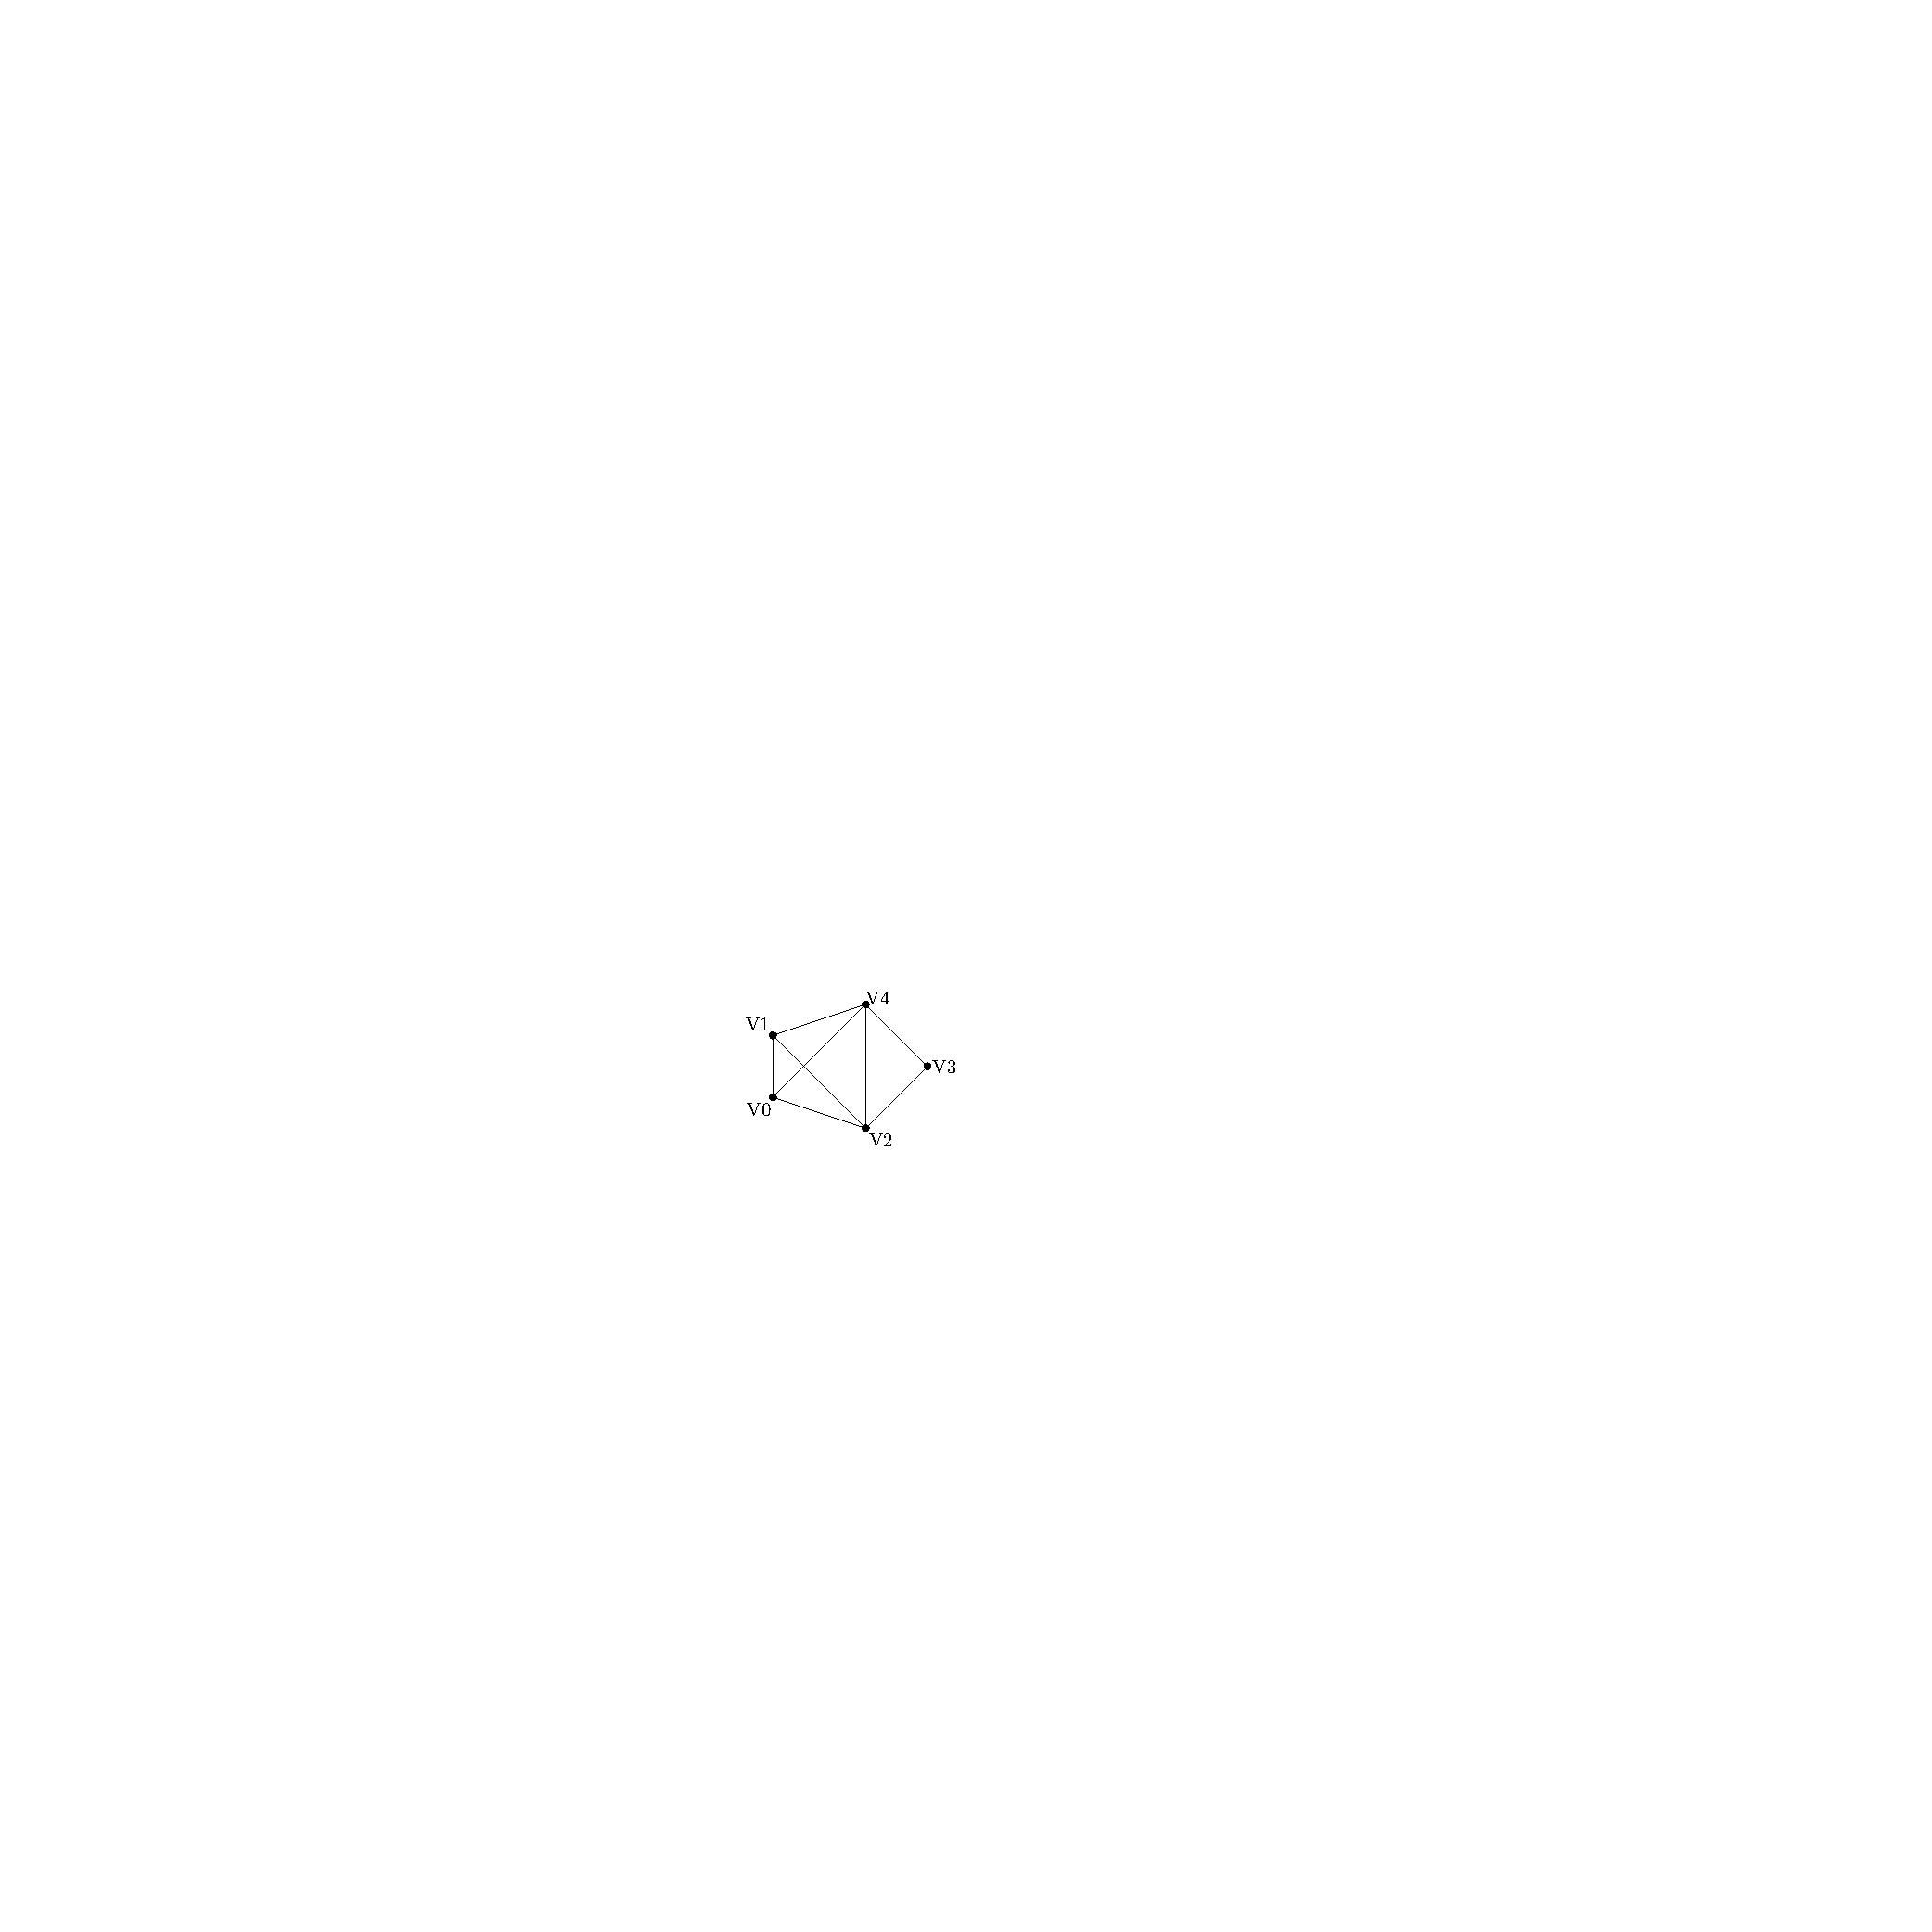
\includegraphics[width=.7\textwidth]{exampleA/straightlineNonplanar}
                \label{fig:exampleAstraightlineNonplanar}
        \end{figure}
        \begin{figure}[h]
                \centering
                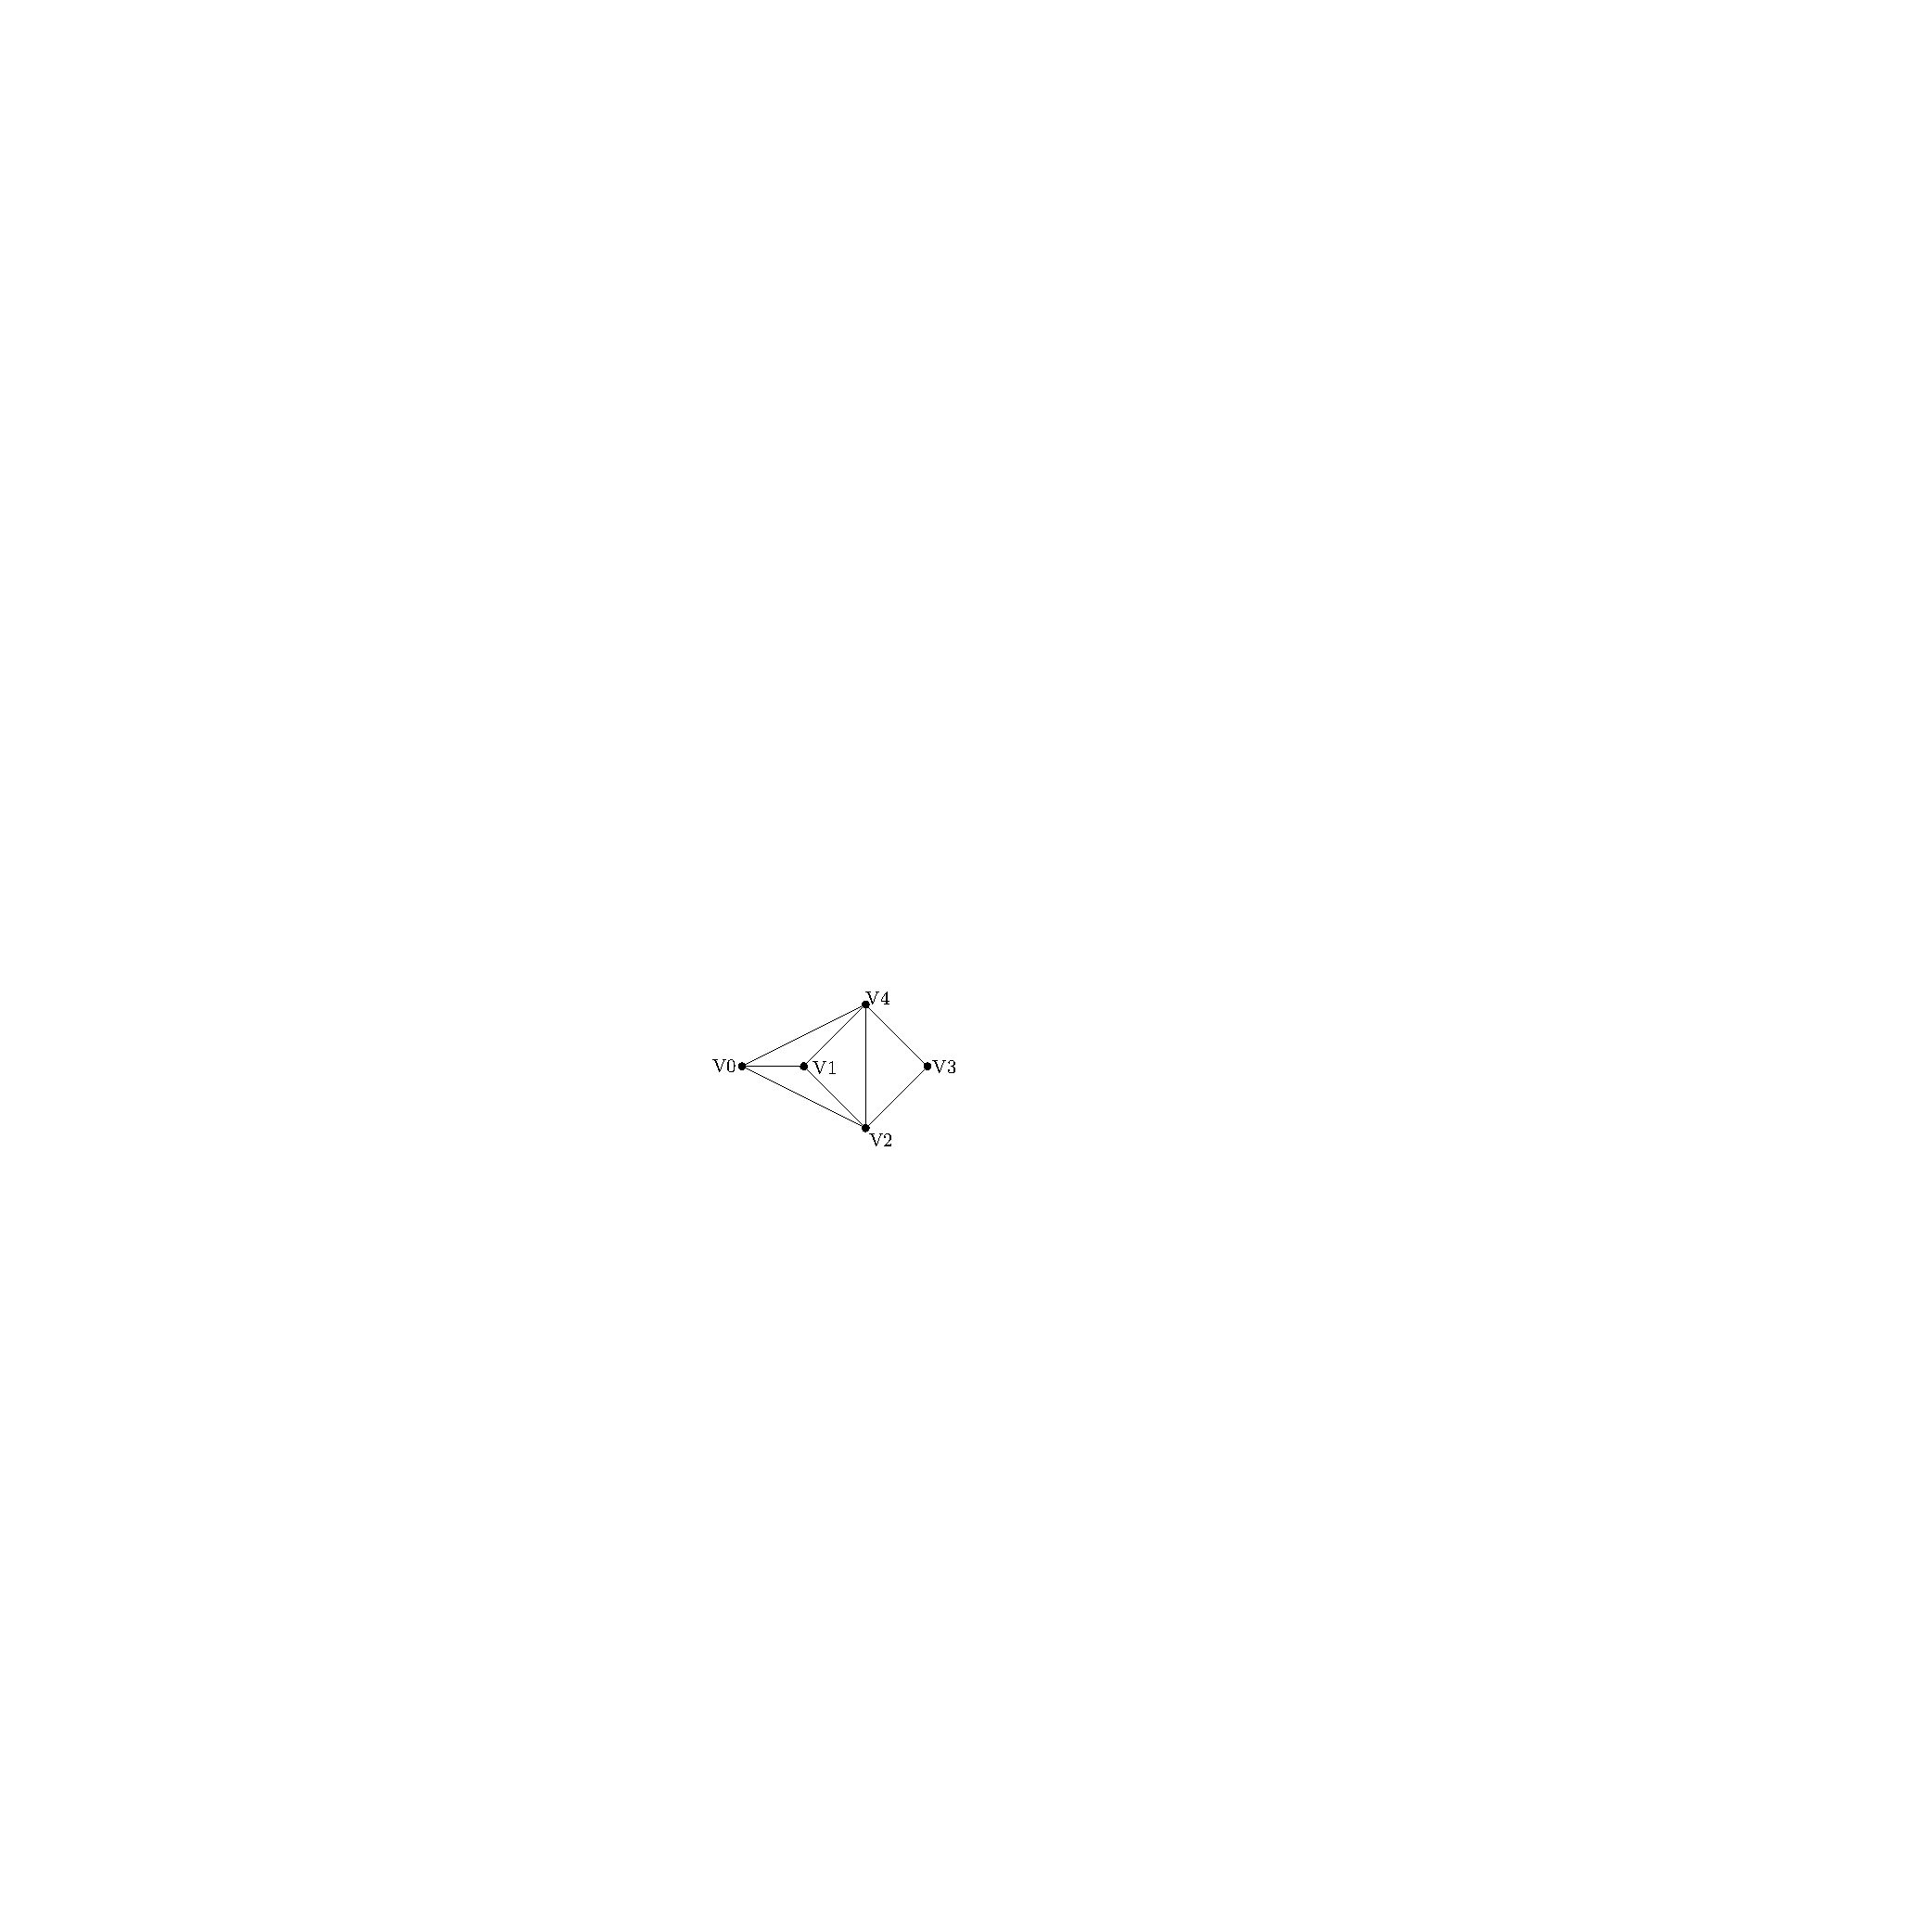
\includegraphics[width=.7\textwidth]{exampleA/straightline}
                \label{fig:exampleAstraightline}
        \end{figure}
\end{column}
\end{columns}
\end{frame}


\begin{frame}
  \frametitle{$st$-Ordnung}
\begin{columns}[c]
\begin{column}{5cm}
  \begin{itemize}[<+->]
    \item Reihenfolge der Knoten
    \item je min. ein Vorgänger und Nachfolger
    \item $s$ erster, $t$ letzter Knoten
    \item Voraussetzung: Graph zweifach zusammenhängend
    \item Berechnung mit dem Algorithmus von Even und Tarjan~\cite{even+tarjan-75}
    \item Zeichenalgorithmus platziert Knoten in Reihenfolge der $st$-Ordnung
  \end{itemize}
\end{column}
\begin{column}{5cm}
        \begin{figure}[h]
                \centering
                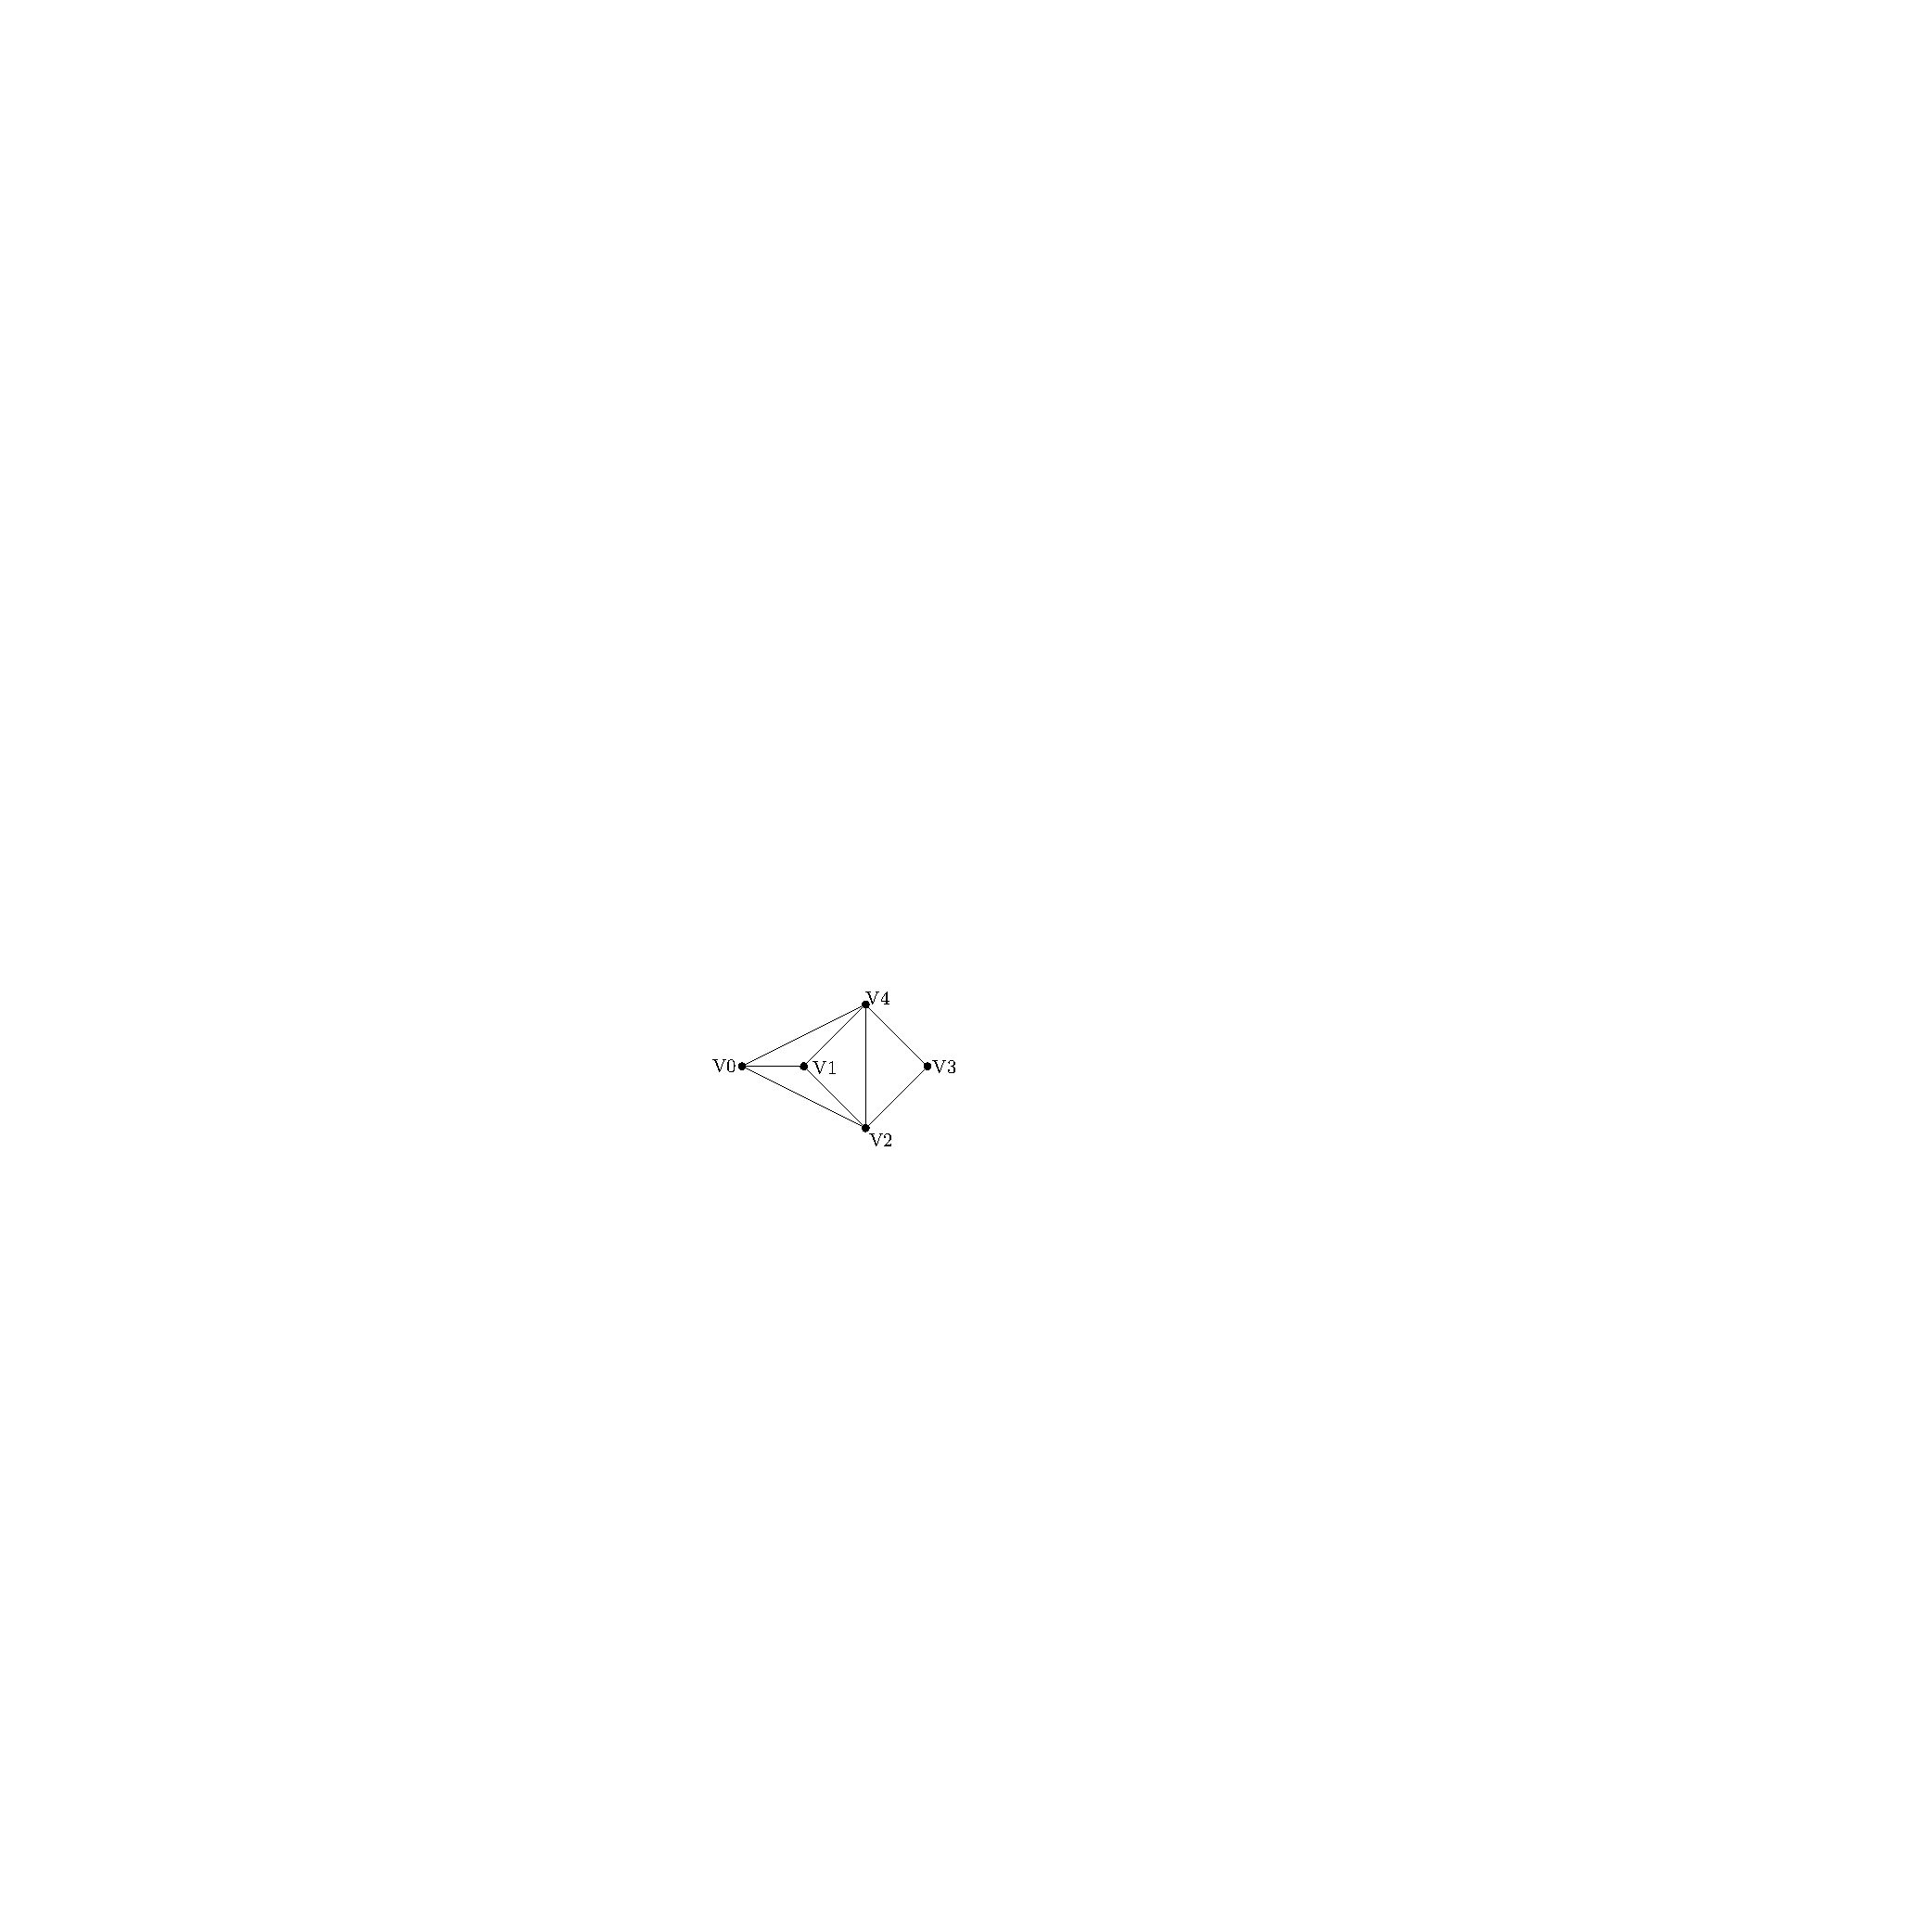
\includegraphics[width=1\textwidth]{exampleA/straightline}
                \caption{Knotenzahlen sind $st$-Ordnung. Vertauscht man V1 und V3, so hat V1 nur nachfolgende Knoten. }
                \label{fig:exampleAstraightline}
        \end{figure}
\end{column}
\end{columns}
\end{frame}


\begin{frame}
  \frametitle{Orthogonale Layouts}
\begin{columns}[c]
\begin{column}{5cm}
  \begin{itemize}[<+->]
    \item Knoten auf einem Gitter
    \item Kanten nur horizontal und vertikal
    \item Vier Ports für Kanten an jedem Knoten
    \item Maximaler Grad ist~4
    \item Berechnung mit Algorithmus von Liu et al.~\cite{liu+etal-98}.
  \end{itemize}
\end{column}
\begin{column}{5cm}
\begin{figure}[h]
  \centering
  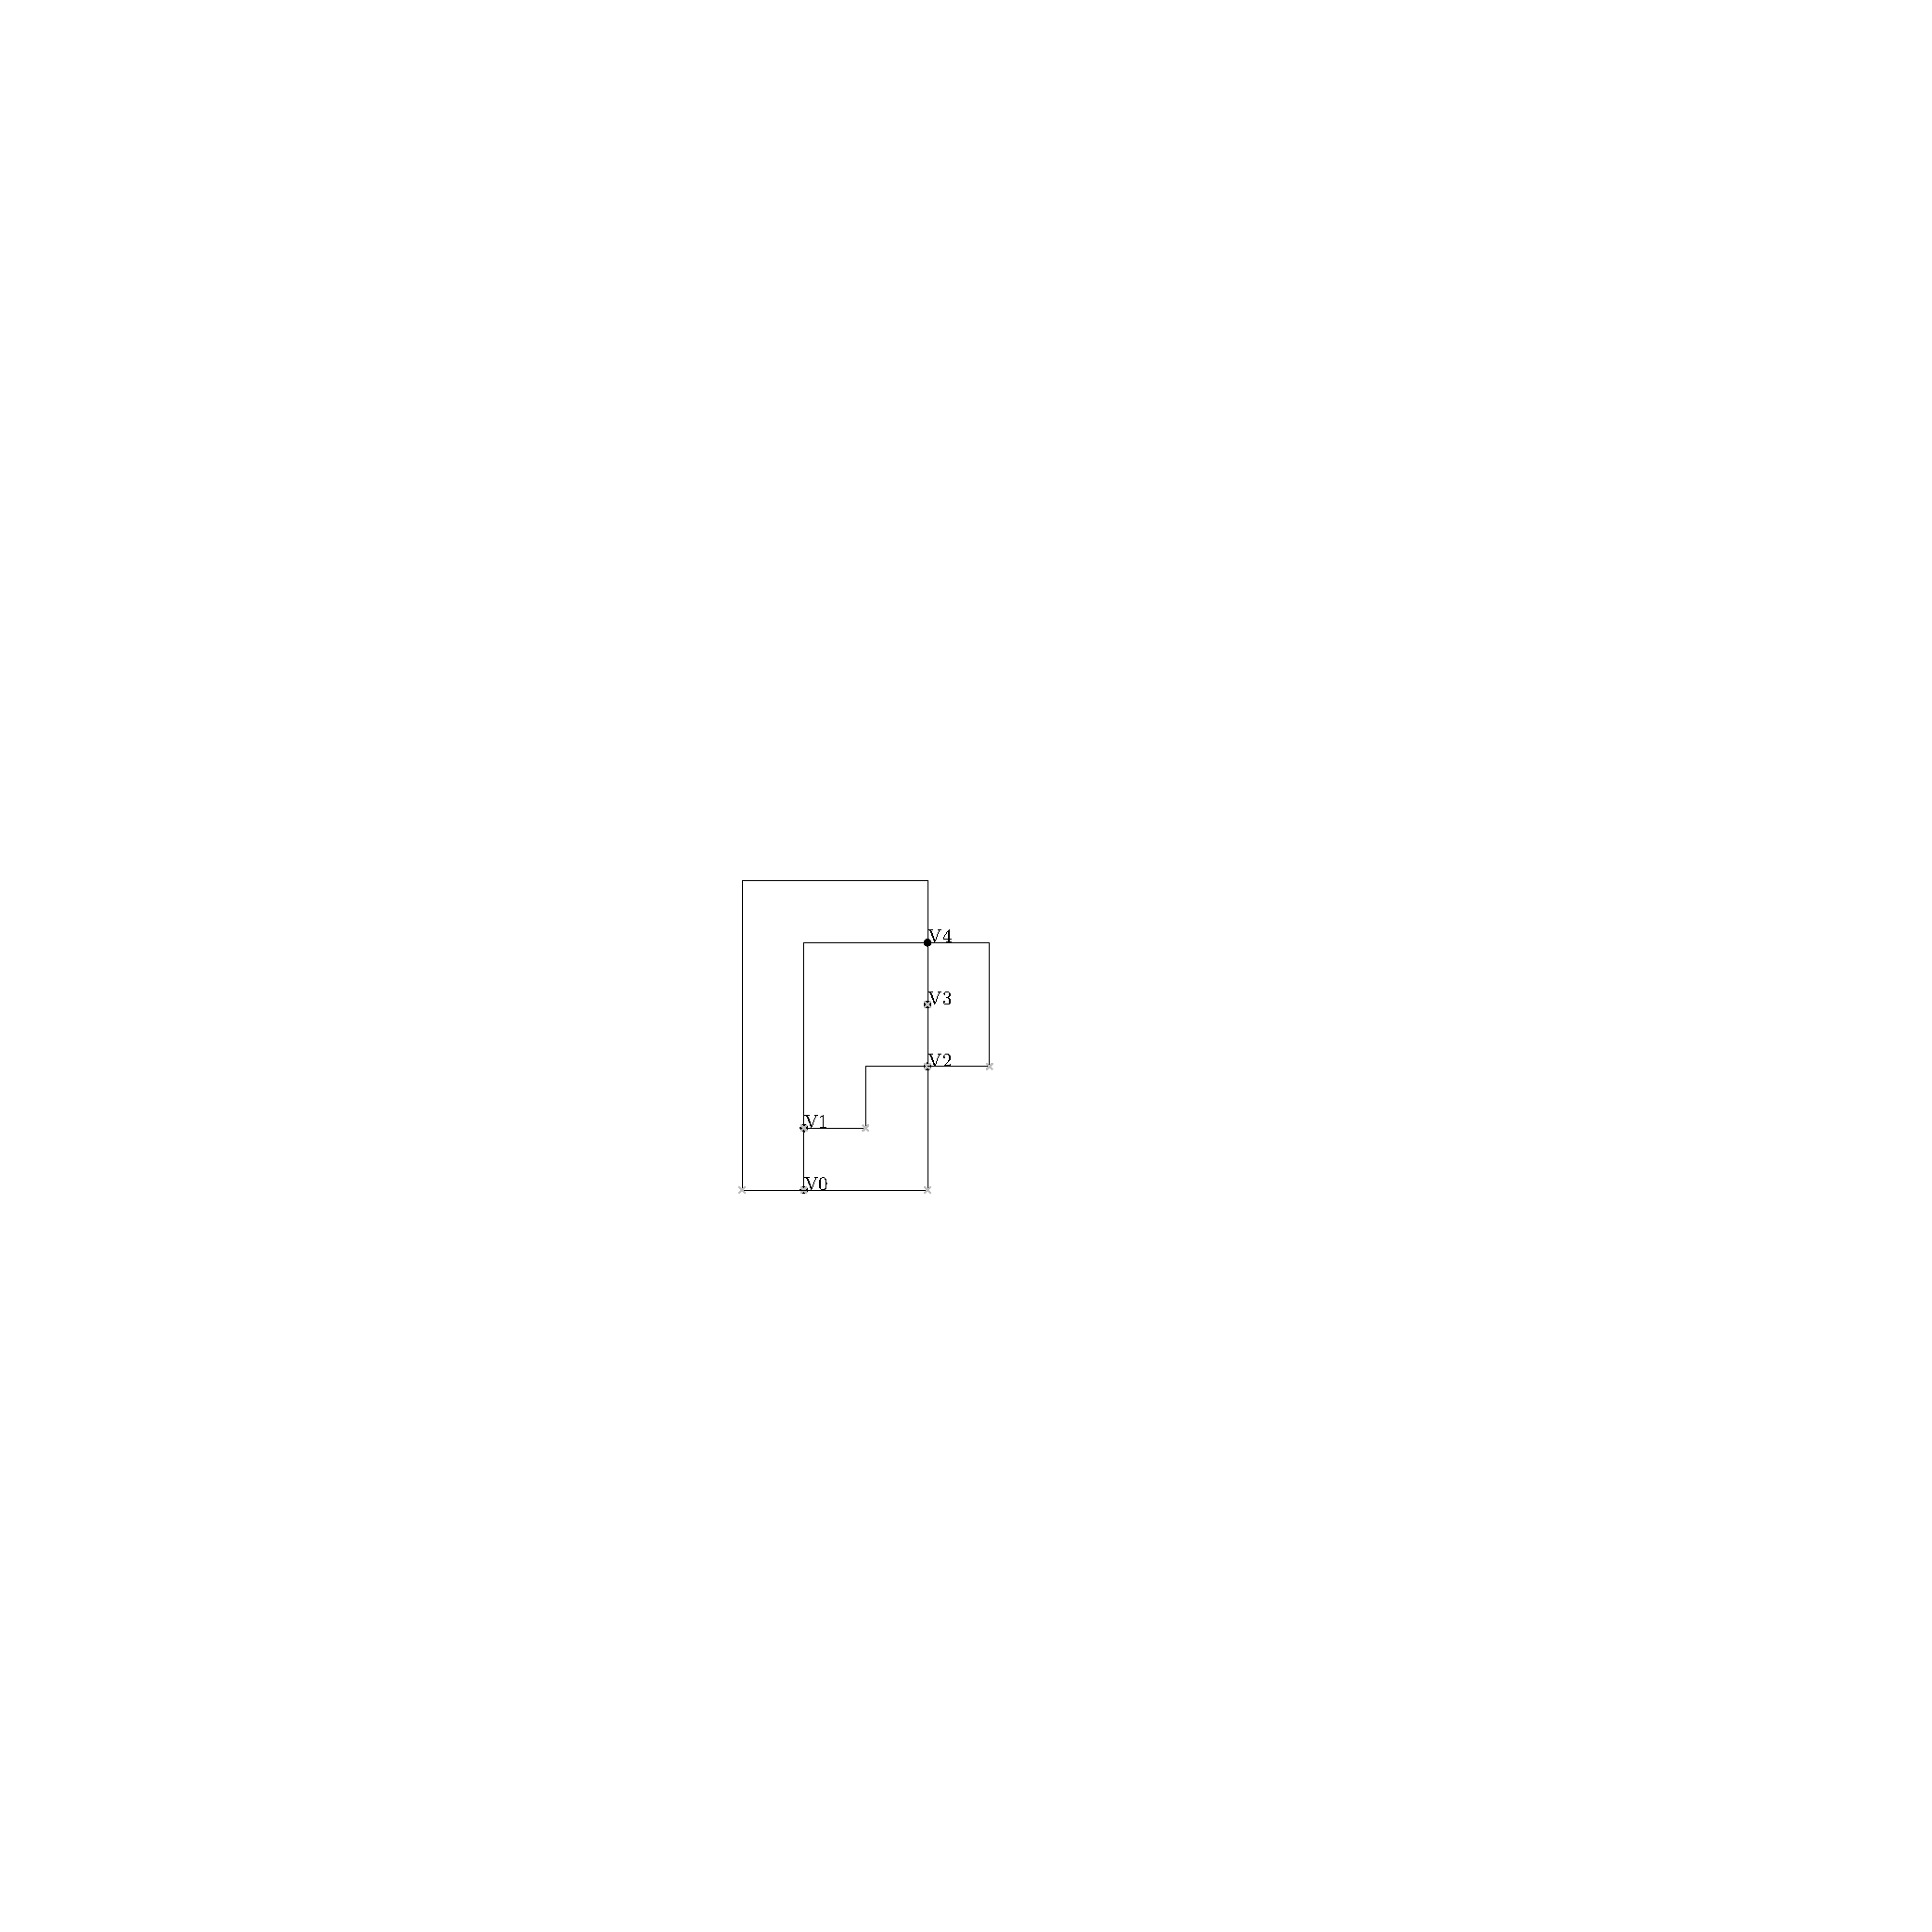
\includegraphics{exampleA/orthogonalNocompress}
  \caption{Orthogonales Layout des Beispielgraphen}
  \label{fig:exampleAorthogonalNocompress}
\end{figure}
\end{column}
\end{columns}
\end{frame}


\begin{frame}
  \frametitle{Der Algorithmus von Liu et al.}
  \begin{itemize}[<+->]
    \item Spezielle Portzuweisung aus planarer Einbettung
    \item Kante hat max. 3 Segmente
    \item Von unten nach oben
    \item Reihenfolge der $st$-Ordnung
    \item Kantenparition in ein- und ausgehend $st$-Ordnung
  \end{itemize}
\end{frame}

% TODO: use outdeg?
\begin{frame}
  \frametitle{Portzuweisung im Algorithmus von Liu et al.}

Portzuweisung eingehender Kanten je Eingangsgrad. Fett sind eingehende Kanten, gestrichelt mögliche ausgehende Kanten.

\begin{columns}[b]
\begin{column}{2cm}
        \begin{figure}[h]
                \centering
                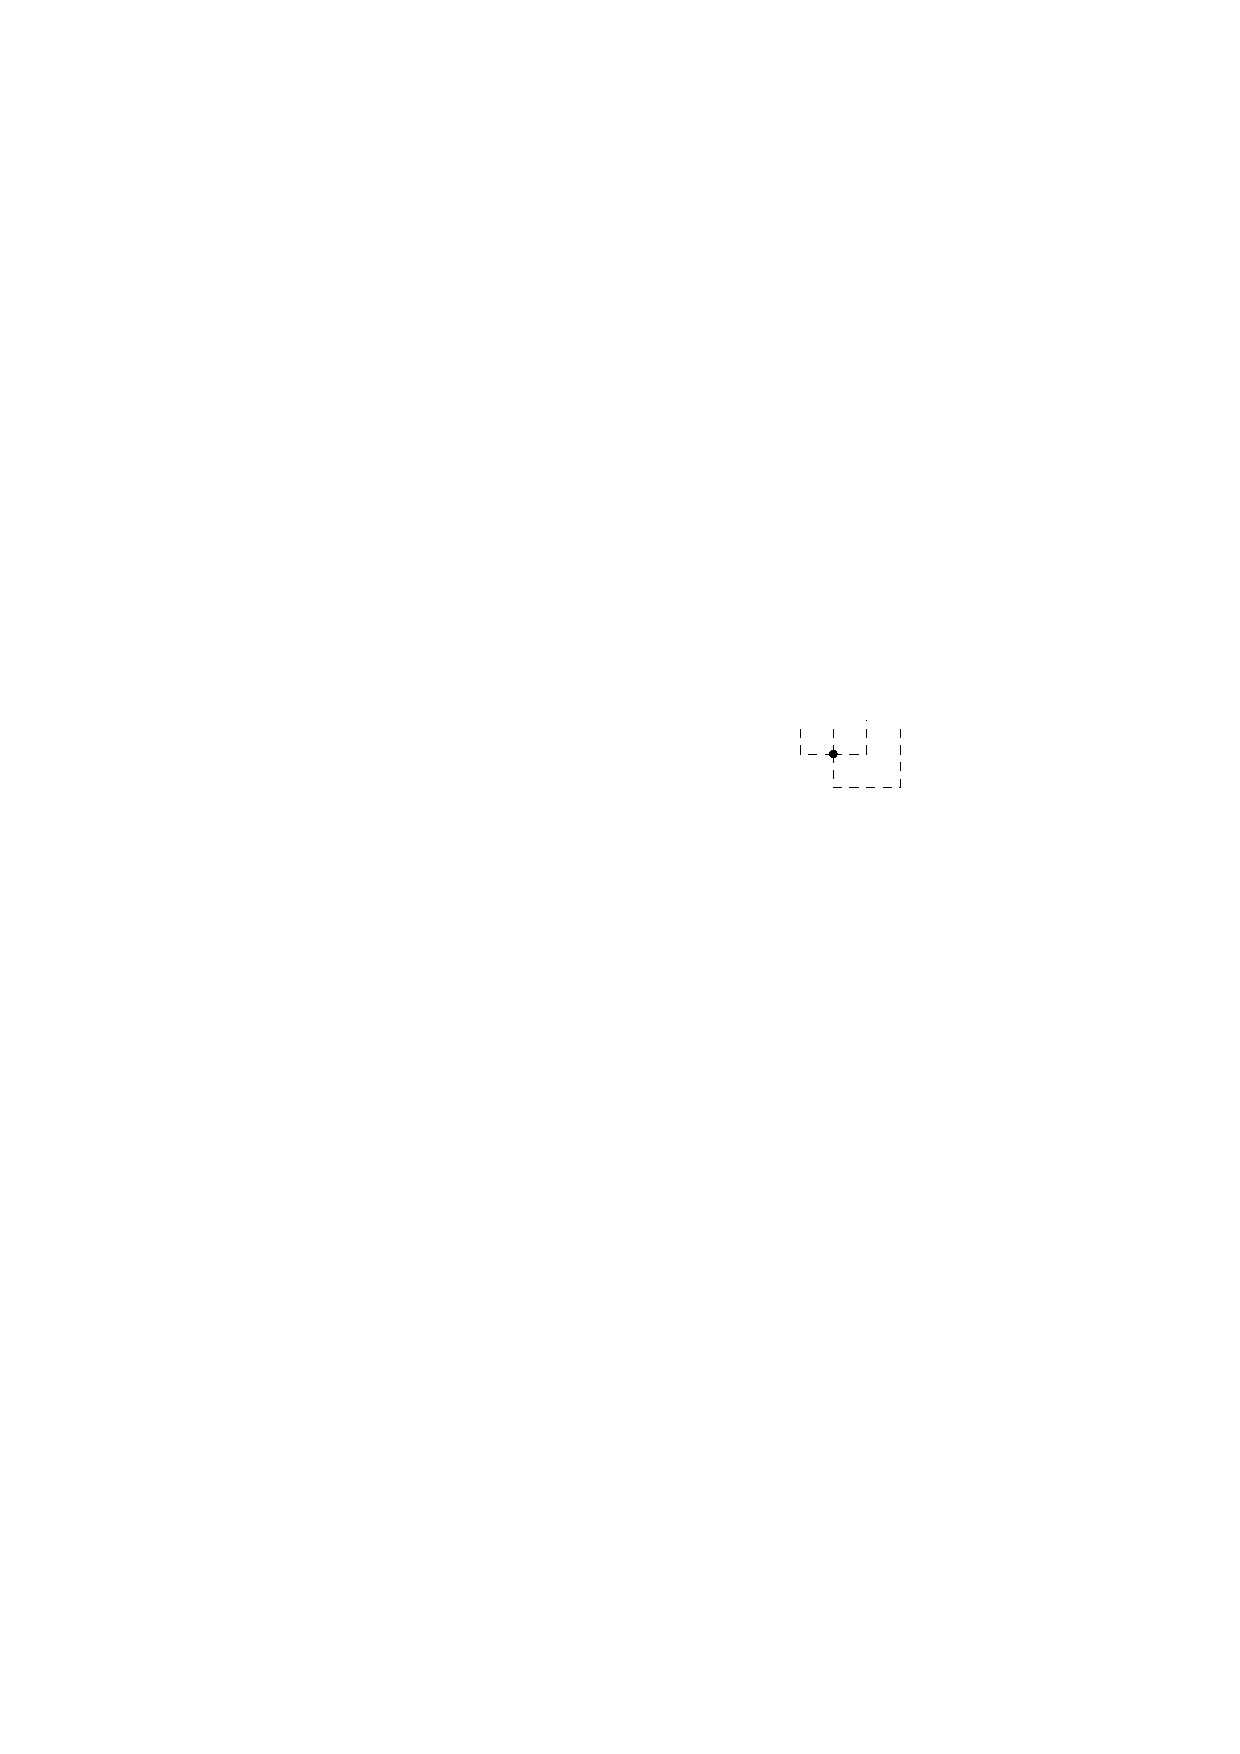
\includegraphics[scale=.8]{oc3_embed/incoming/indeg0}
                \caption{0}
        \end{figure}
\end{column}
\begin{column}{2cm}
        \begin{figure}[h]
                \centering
                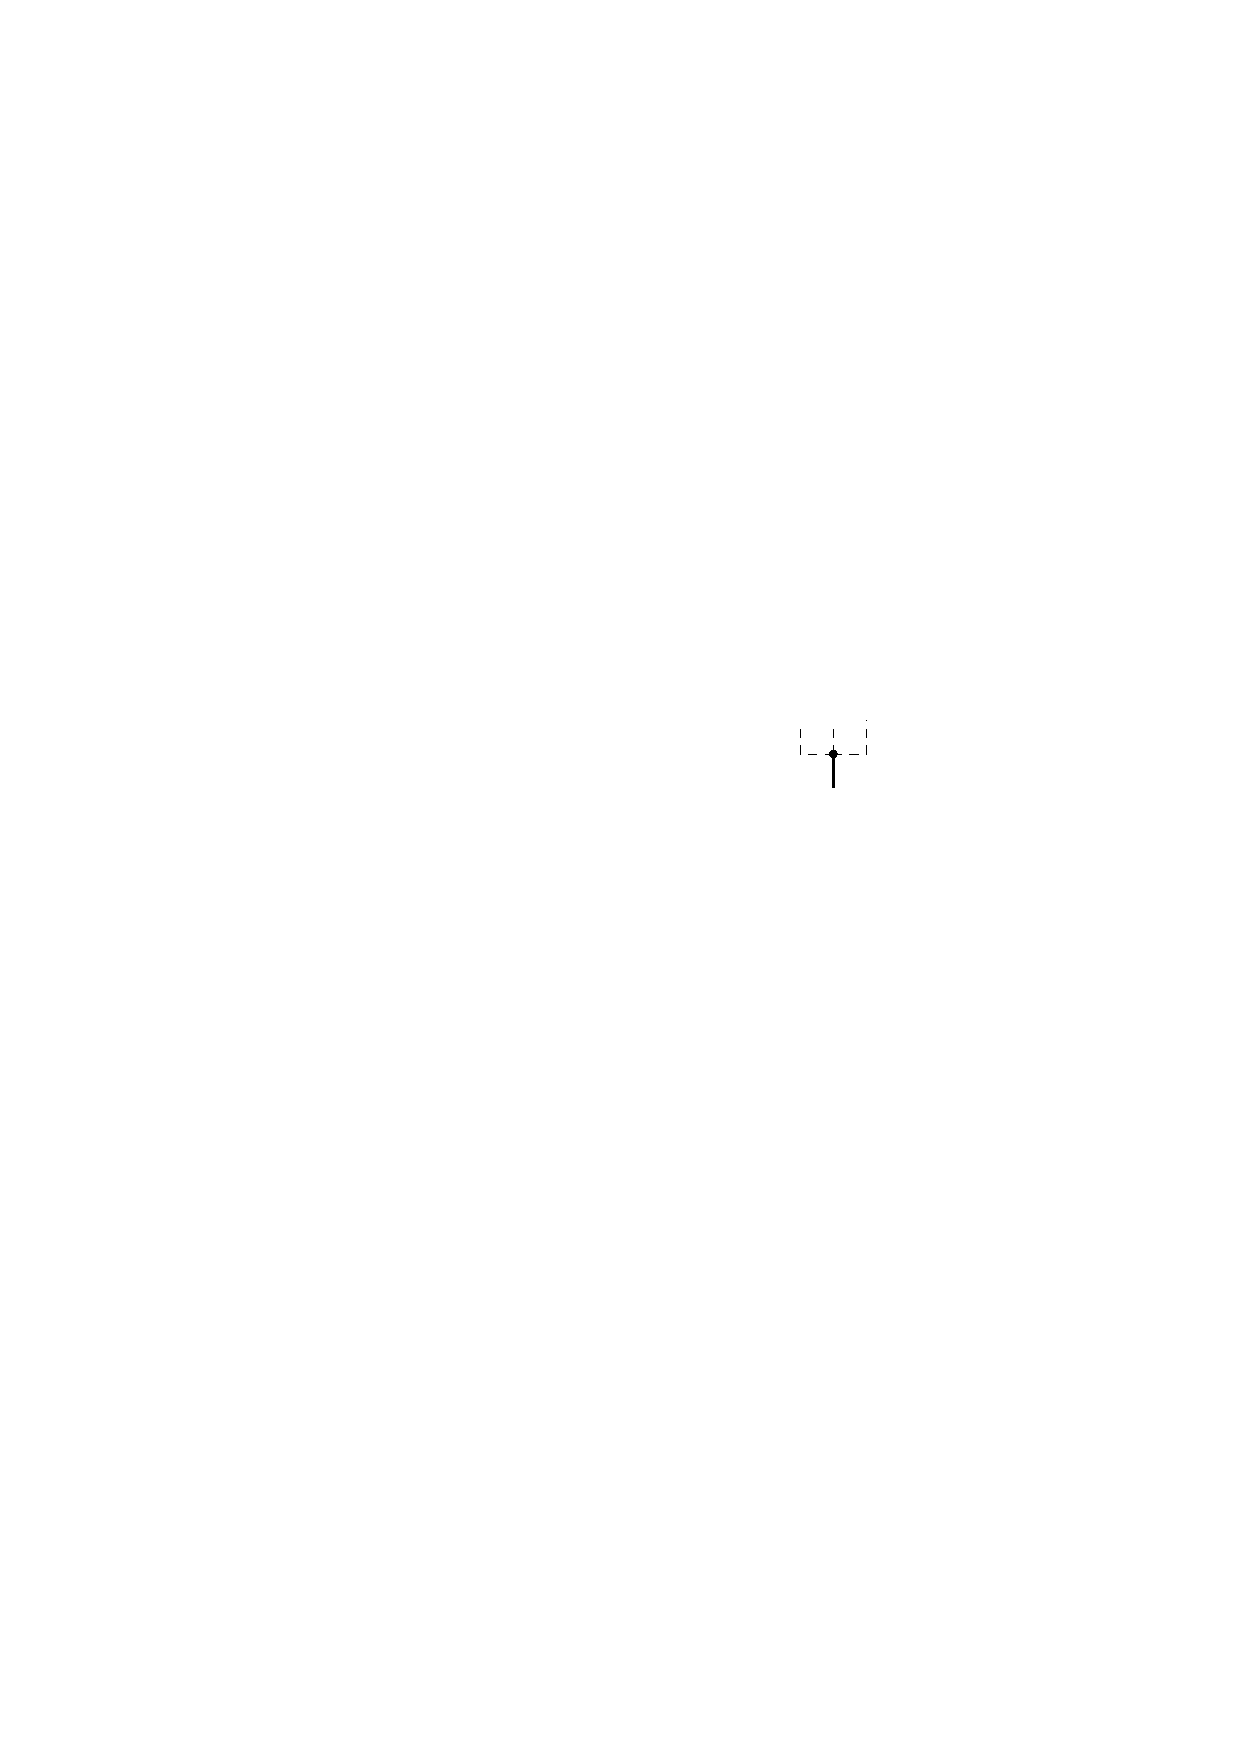
\includegraphics[scale=.8]{oc3_embed/incoming/indeg1}
                \caption{1}
        \end{figure}
\end{column}
\begin{column}{2cm}
        \begin{figure}[h]
                \centering
                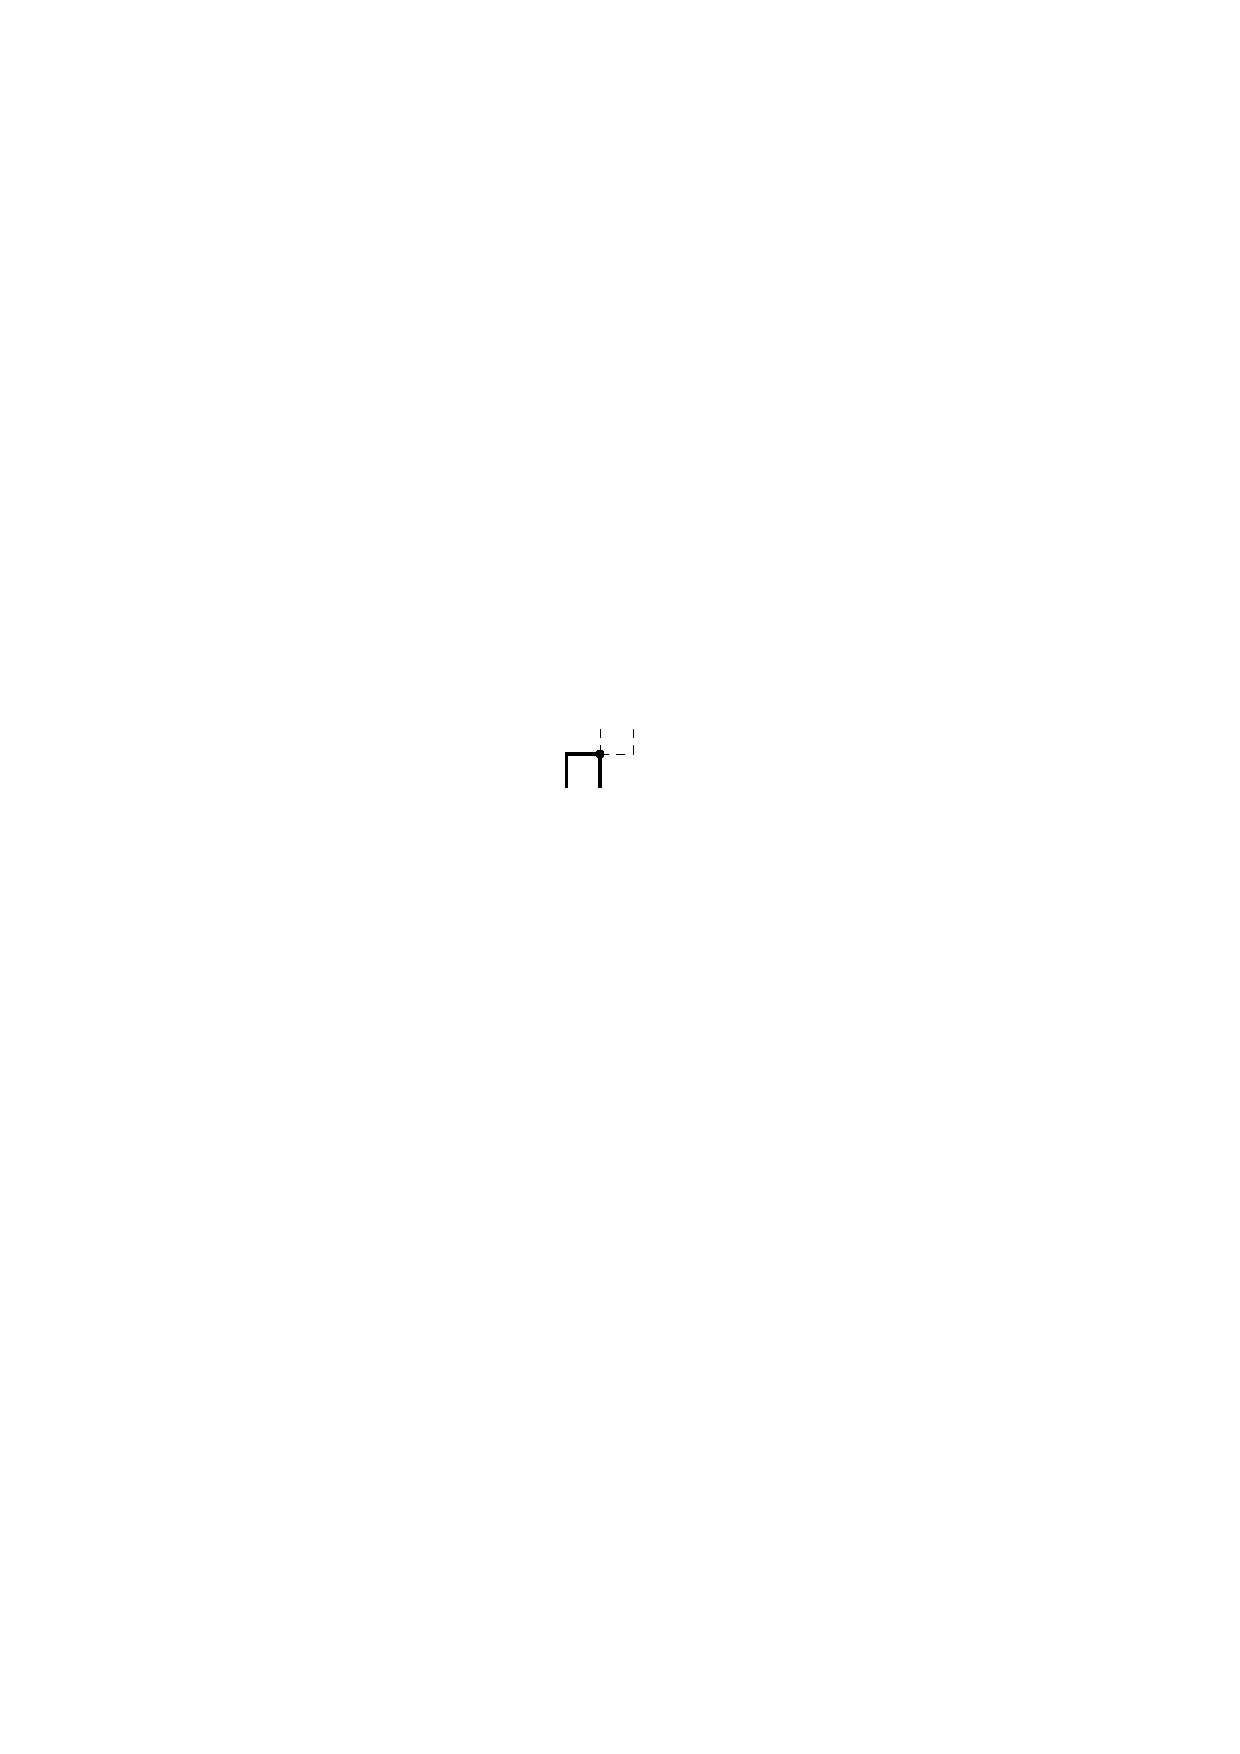
\includegraphics[scale=.8]{oc3_embed/incoming/indeg2}
                \caption{2}
        \end{figure}
\end{column}
\begin{column}{2cm}
        \begin{figure}[h]
                \centering
                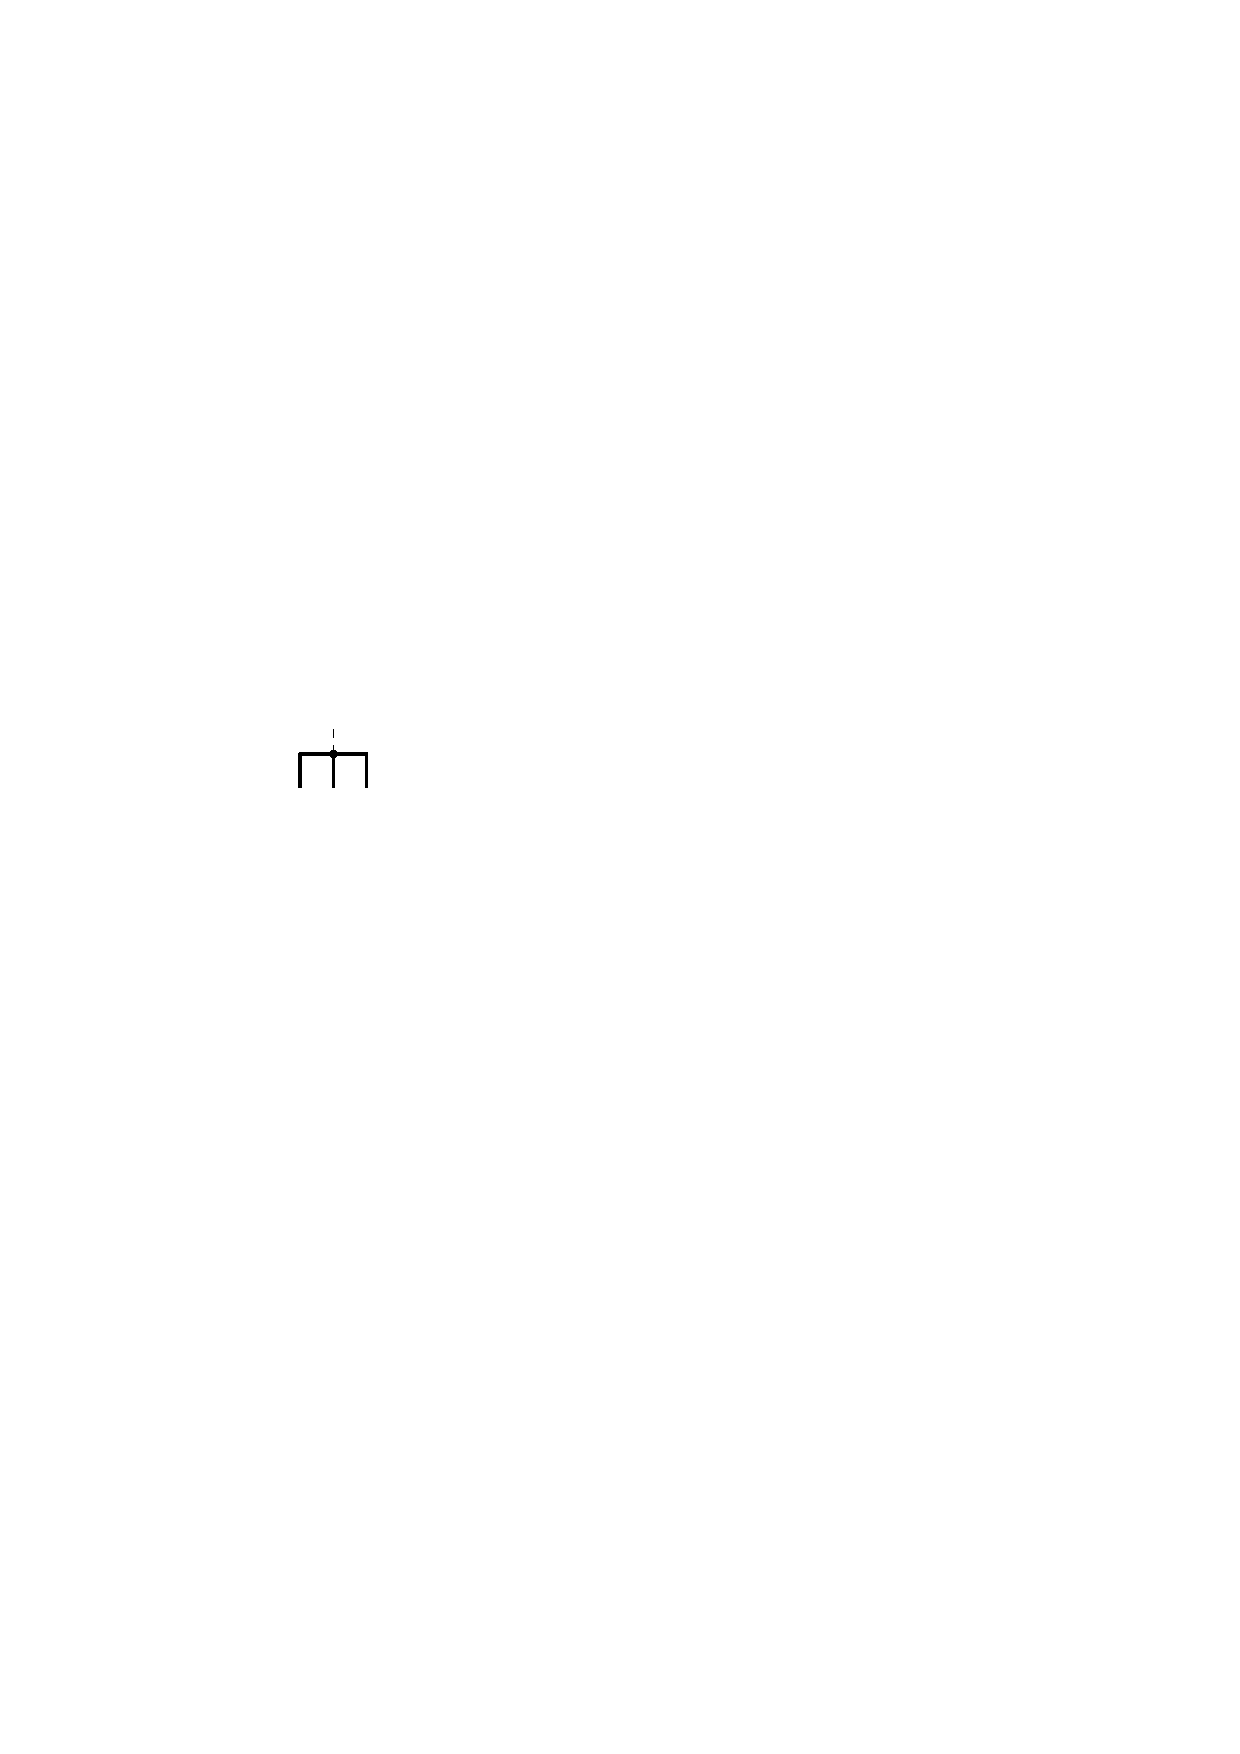
\includegraphics[scale=.8]{oc3_embed/incoming/indeg3}
                \caption{3}
        \end{figure}
\end{column}
\begin{column}{2cm}
        \begin{figure}[h]
                \centering
                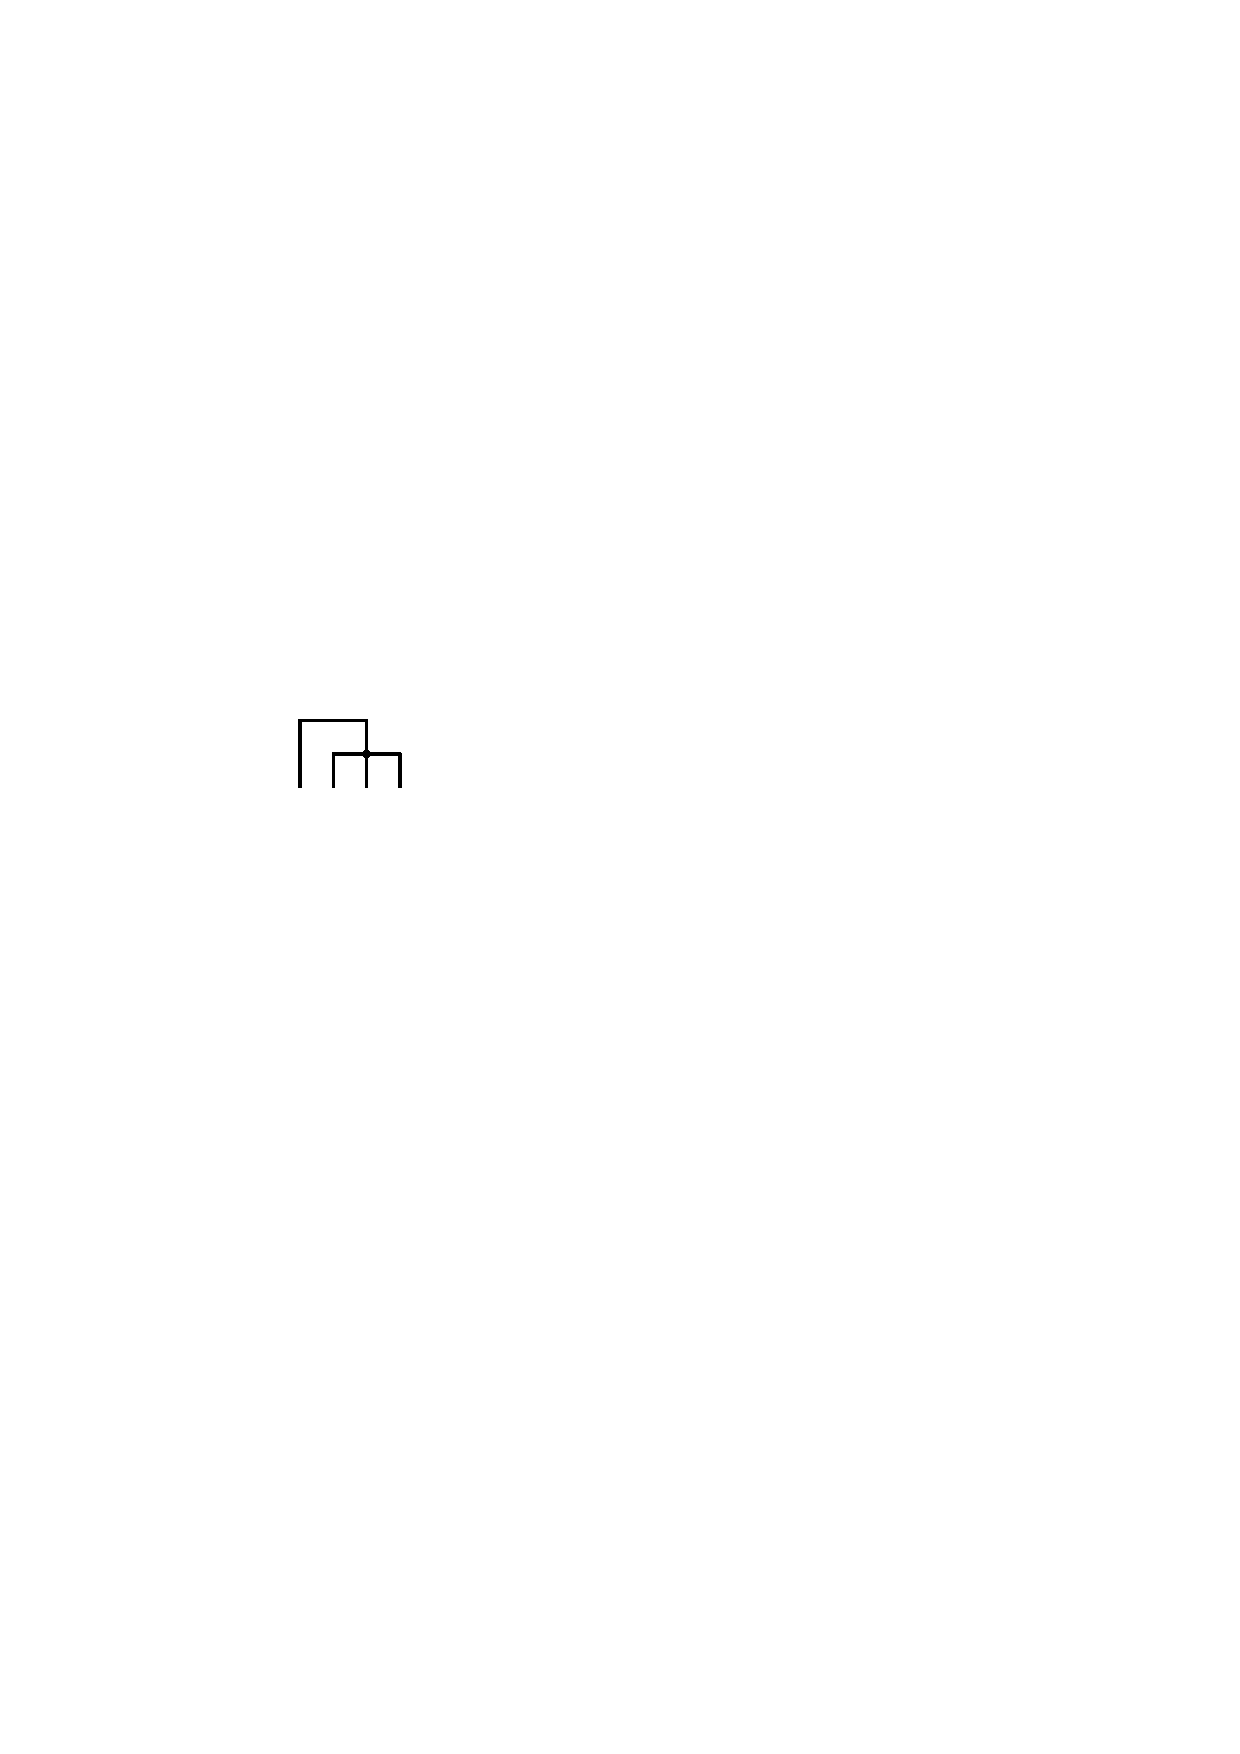
\includegraphics[scale=.8]{oc3_embed/incoming/indeg4}
                \caption{4}
        \end{figure}
\end{column}
\end{columns}
\end{frame}

\begin{frame}
  \frametitle{Beispiel zum Algorithmus von Liu et al.}
\begin{columns}[t]
\begin{column}{5cm}
\begin{figure}[h]
  \centering
  \includegraphics<1>[page=1]{exampleA/orthogonalNocompress_liuWalkthrough}
  \includegraphics<2>[page=2]{exampleA/orthogonalNocompress_liuWalkthrough}
  \includegraphics<3>[page=3]{exampleA/orthogonalNocompress_liuWalkthrough}
  \includegraphics<4>[page=4]{exampleA/orthogonalNocompress_liuWalkthrough}
  \includegraphics<5>[page=5]{exampleA/orthogonalNocompress_liuWalkthrough}
  \includegraphics<6>[page=6]{exampleA/orthogonalNocompress_liuWalkthrough}
  \includegraphics<7>[page=7]{exampleA/orthogonalNocompress_liuWalkthrough}
\end{figure}
\end{column}
\begin{column}{5cm}
\begin{figure}[h]
  \centering
  \includegraphics<1>[page=1]{exampleA/straightline_liuWalkthrough}
  \includegraphics<2>[page=2]{exampleA/straightline_liuWalkthrough}
  \includegraphics<3>[page=3]{exampleA/straightline_liuWalkthrough}
  \includegraphics<4>[page=4]{exampleA/straightline_liuWalkthrough}
  \includegraphics<5>[page=5]{exampleA/straightline_liuWalkthrough}
  \includegraphics<6>[page=6]{exampleA/straightline_liuWalkthrough}
  \includegraphics<7>[page=7]{exampleA/straightline_liuWalkthrough}
\end{figure}
\end{column}
\end{columns}
\end{frame}




\section{Algorithmus}
\frame{\tableofcontents[currentsection]}

\begin{frame}
  \frametitle{Glatt"=orthogonale Zeichungen}
\begin{columns}[c]
\begin{column}{5cm}
  \begin{itemize}[<+->]
    \item Bekos~et.~al.~\cite{bekos-13}
    \item orthogonal: Koordinatengitter; horizontale, vertikale Segmente, Ports
    \item Glatt: Keine Knicke
    \item Mit Kreisbögen abgerundet
    \item Tangentialer Übergang
  \end{itemize}
\end{column}
\begin{column}{5cm}
\begin{figure}[h]
  \centering
  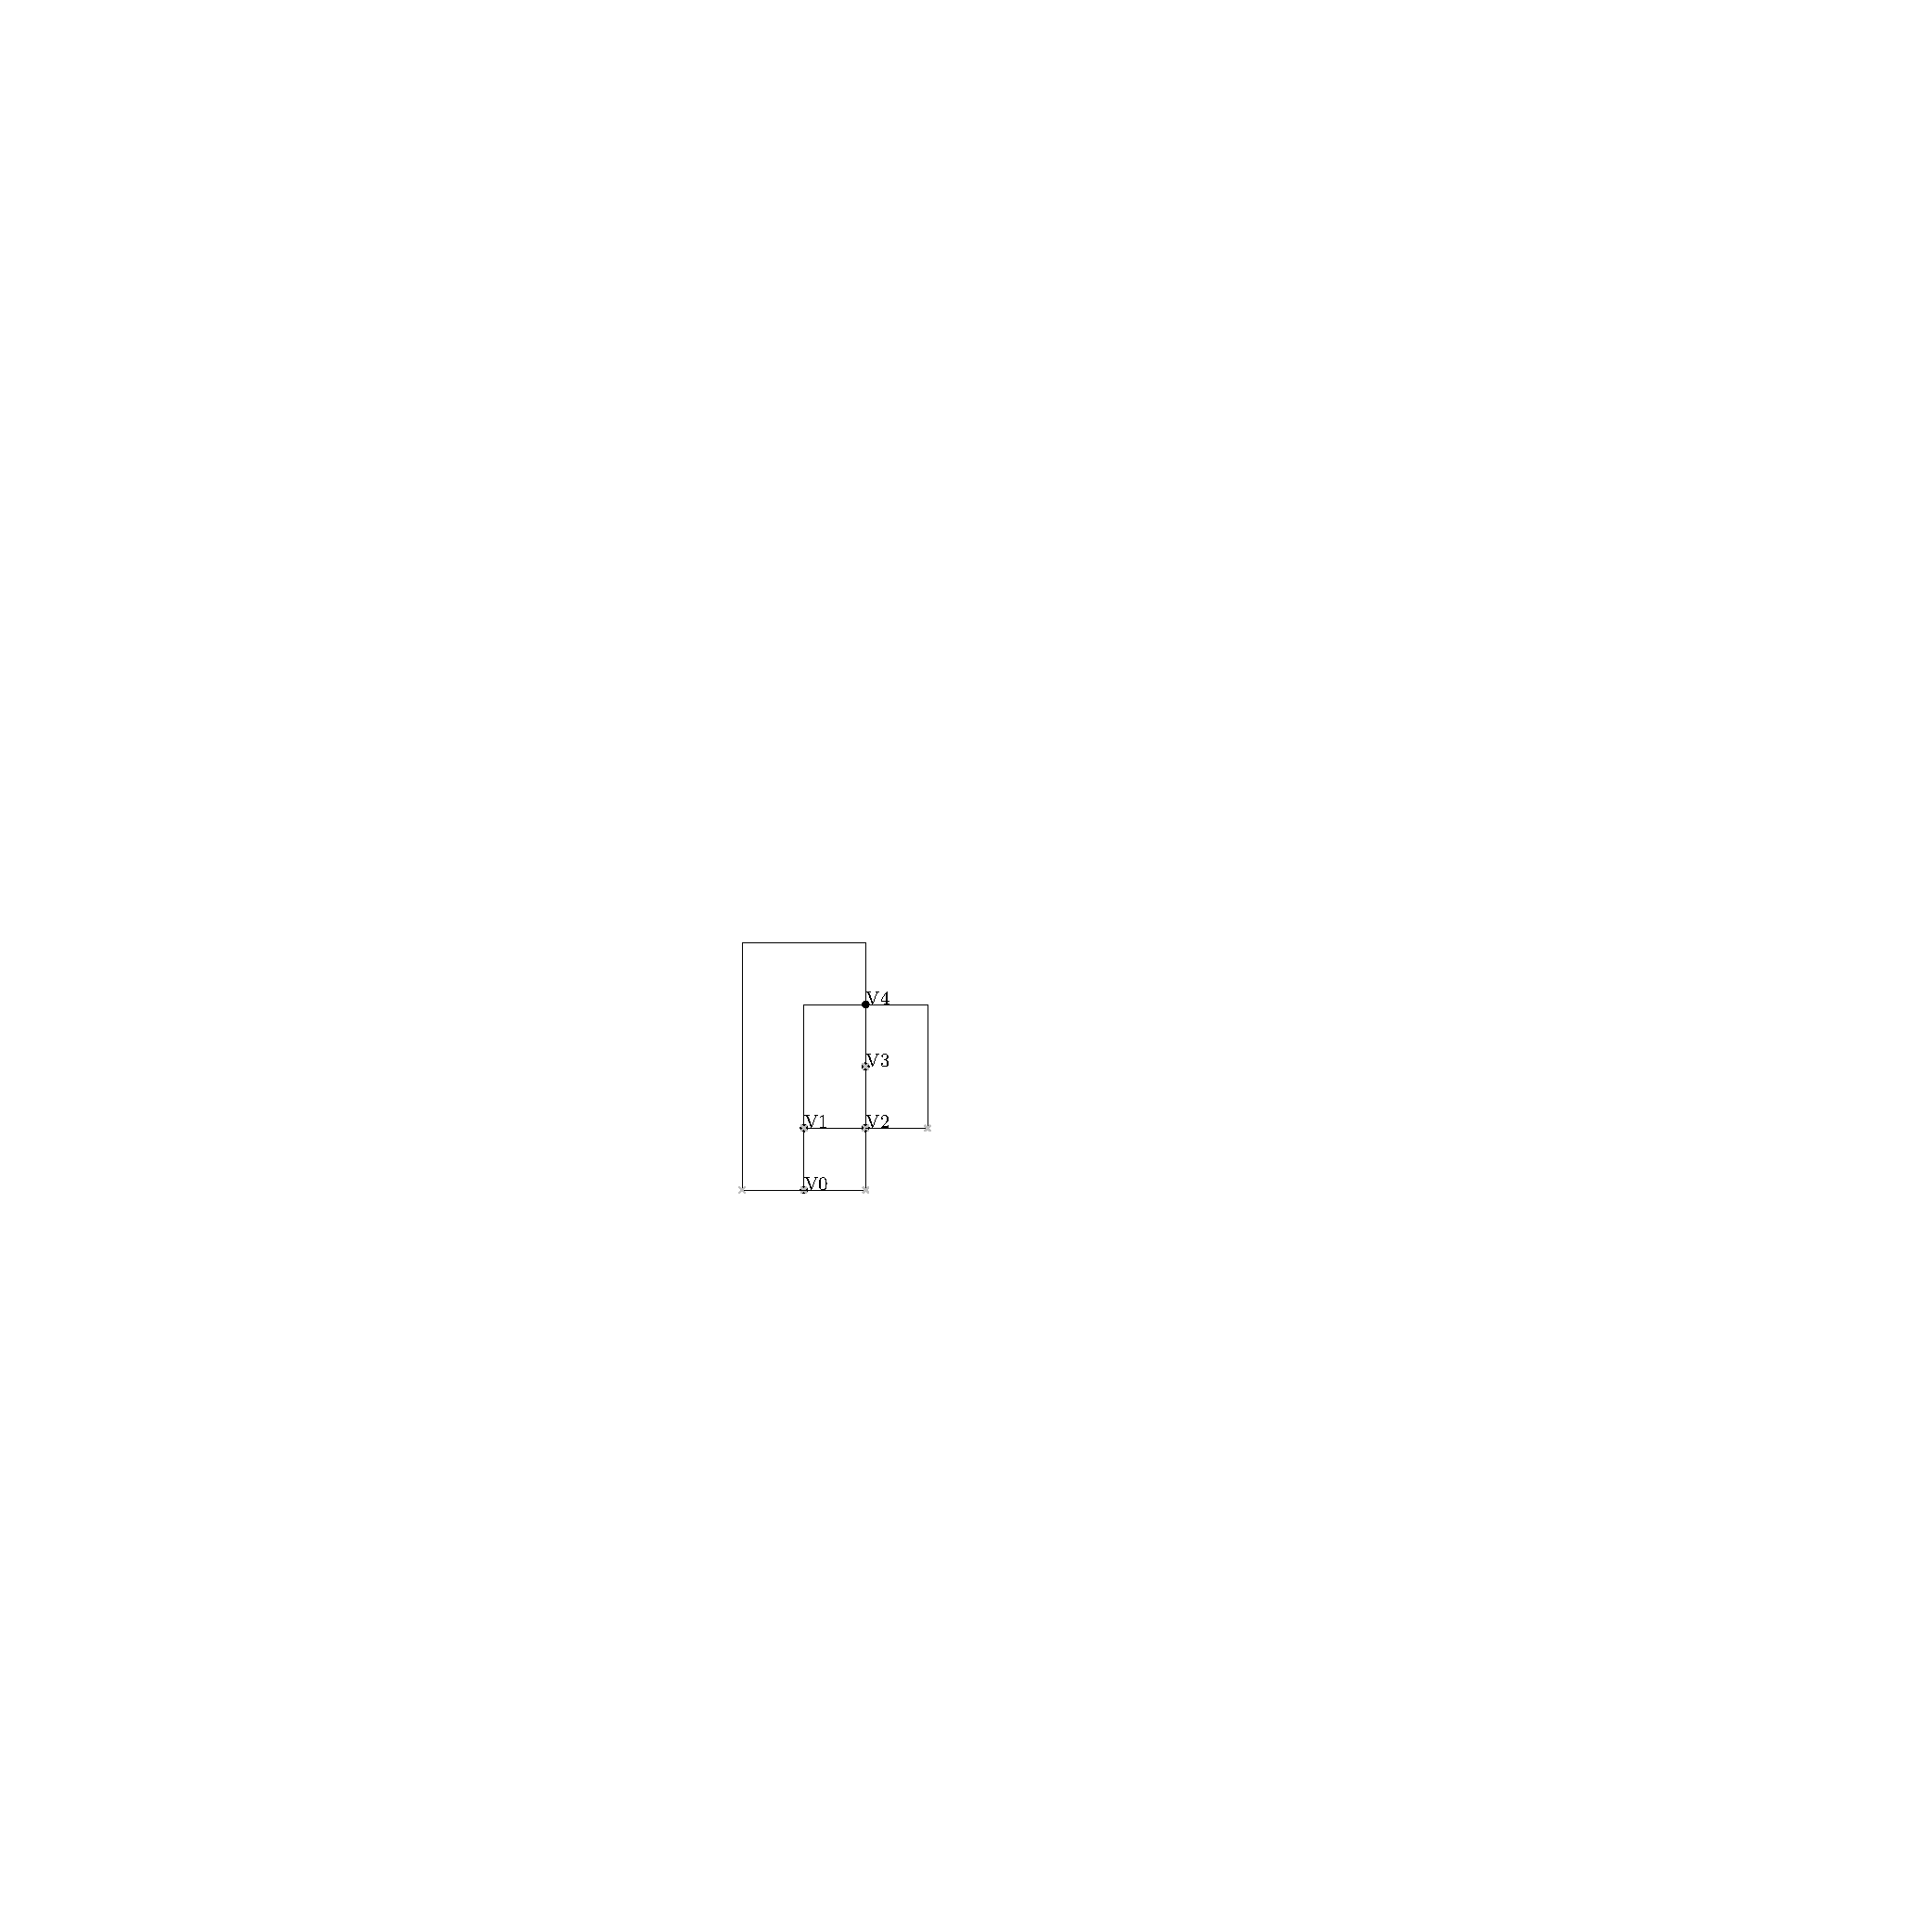
\includegraphics[scale=.7]{exampleA/orthogonalCompress}
  \label{fig:exampleAorthogonalNocompress}
\end{figure}
\begin{figure}[h]
  \centering
  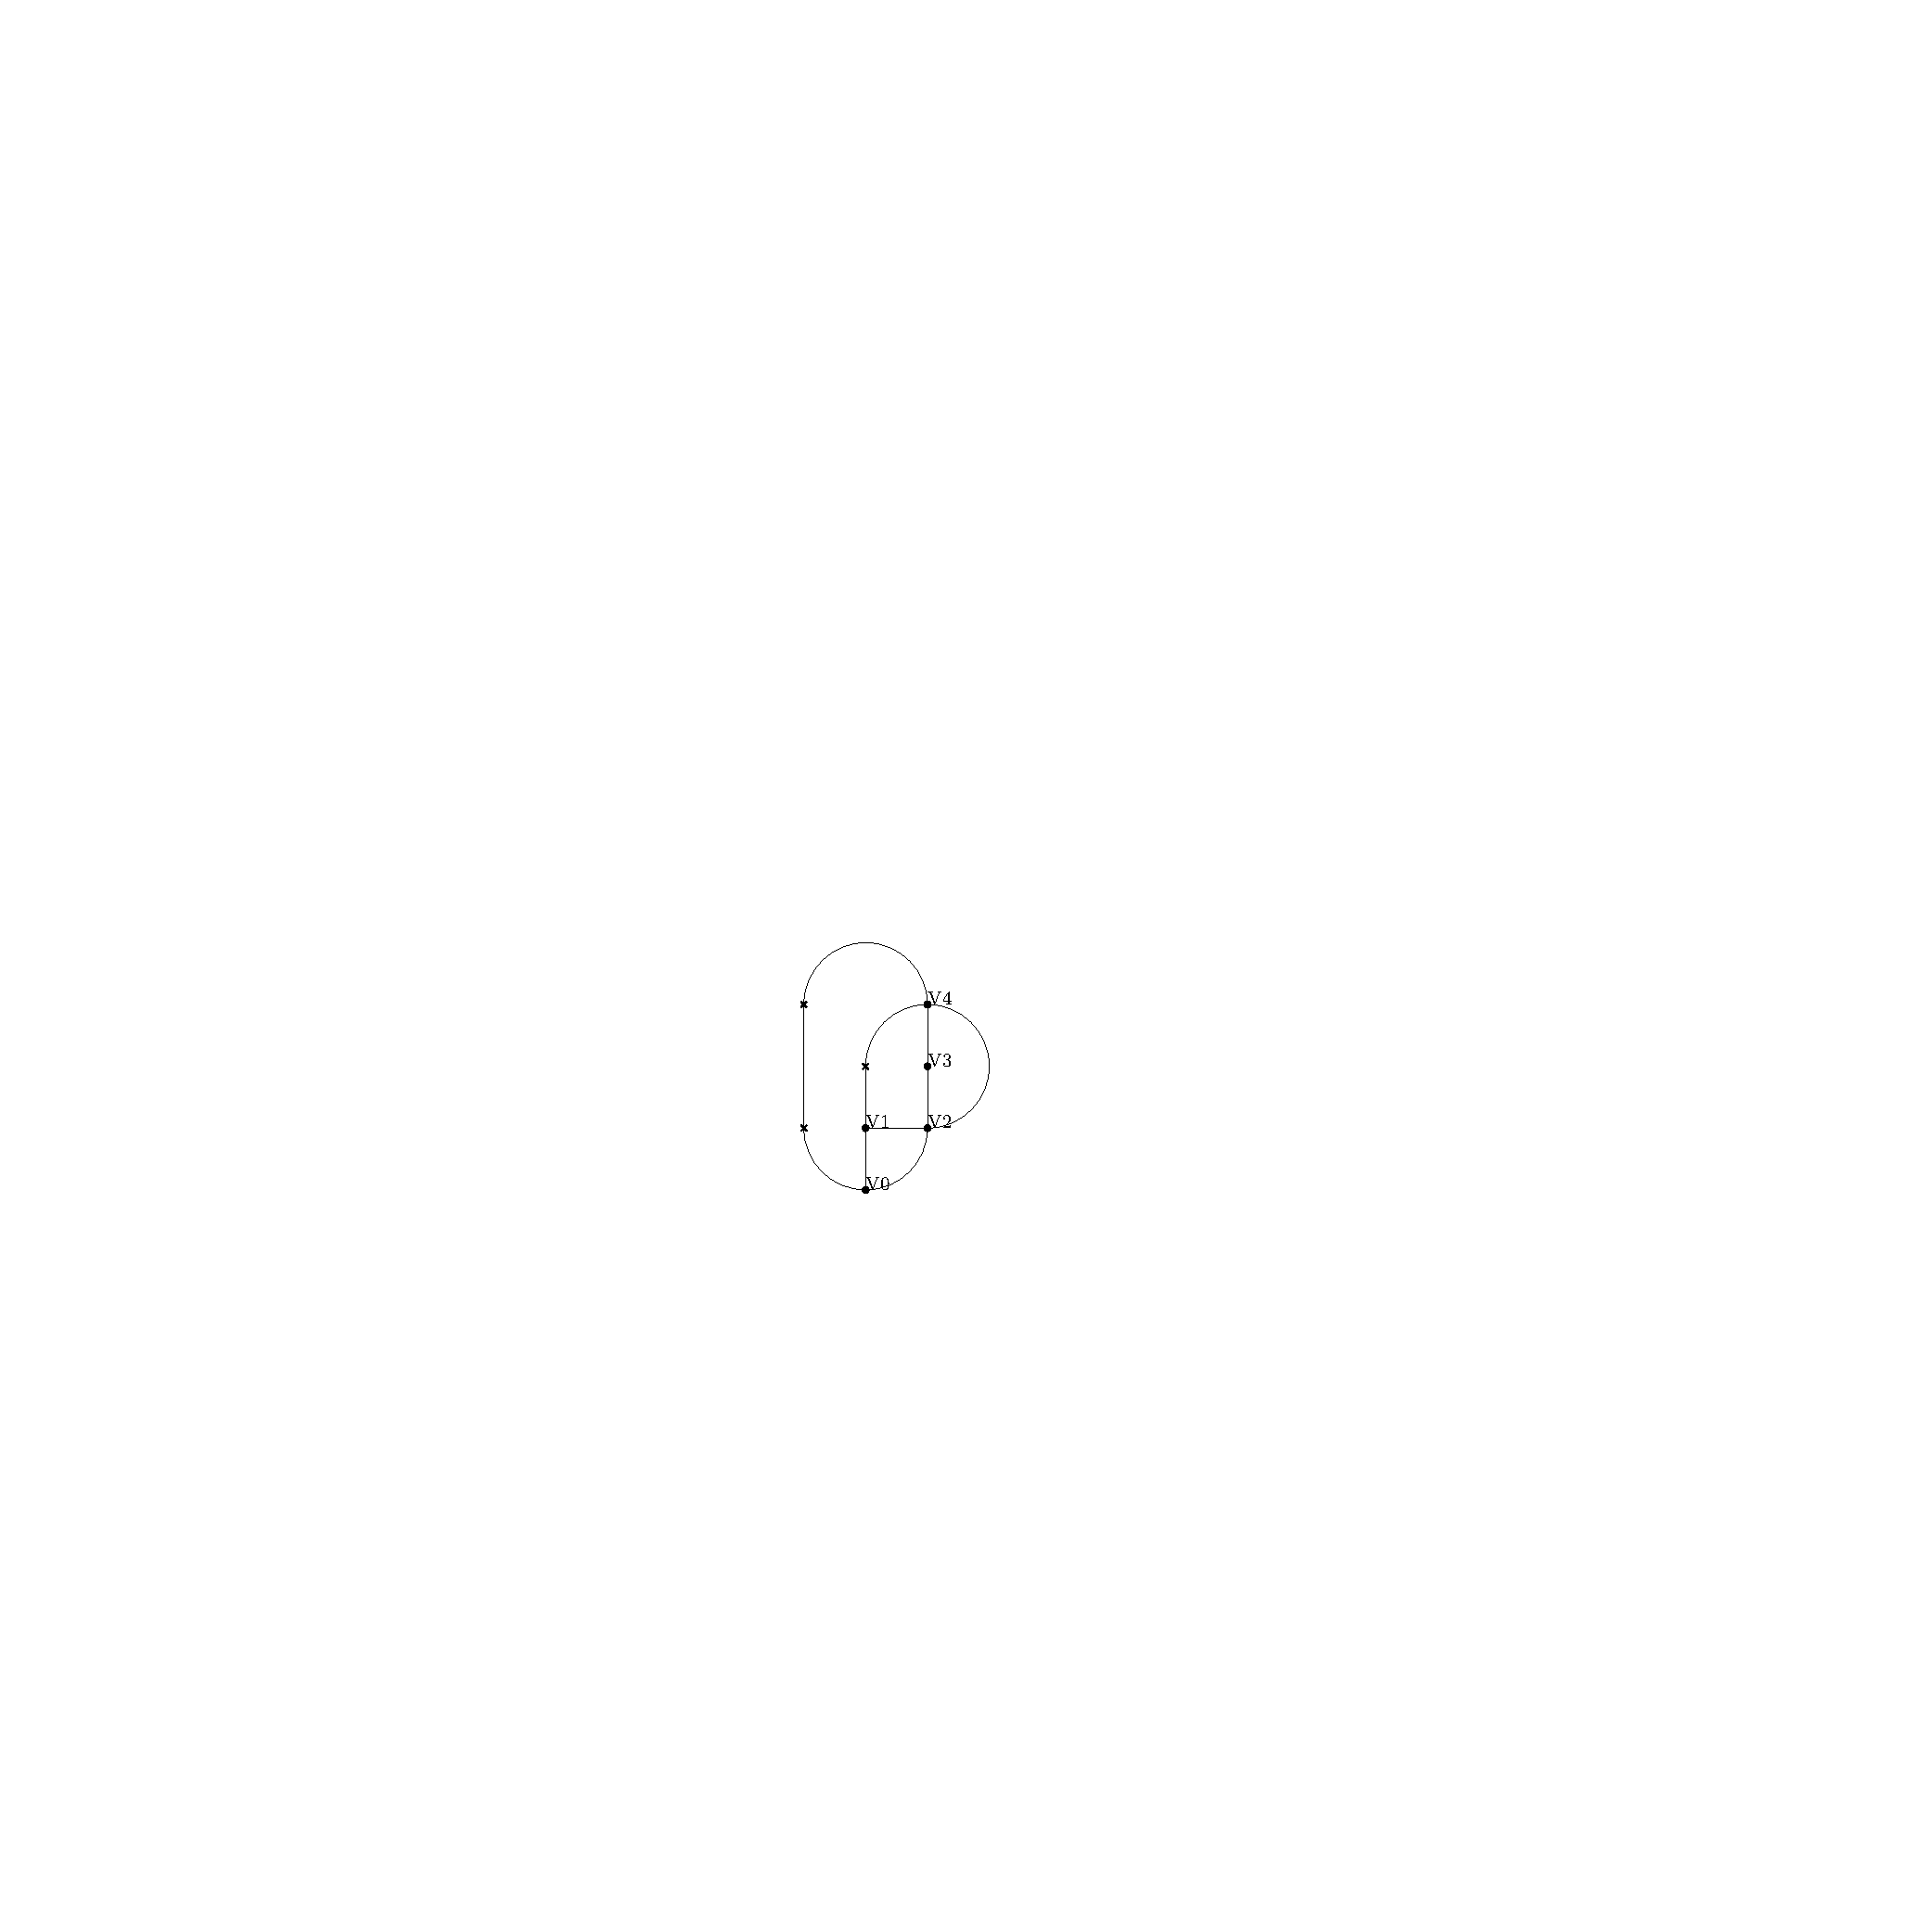
\includegraphics[scale=.7]{exampleA/smoothComplex}
  \label{fig:exampleAsmoothComplex}
\end{figure}
\end{column}
\end{columns}
\end{frame}

\begin{frame}
  \frametitle{Entfernung stufenförmiger Kanten}
  \begin{itemize}[<+->]
    \item Stufenförmige Kanten werden S-förmige Kanten
    \item Alle Stufen-Knoten auf ein Plateau
    \item Höhe des Plateaus berechnen
    \item Mehrere Plateaus mit selber Höhe möglich
  \end{itemize}
\begin{columns}[c]
\begin{column}{5cm}
\begin{figure}[h]
  \centering
  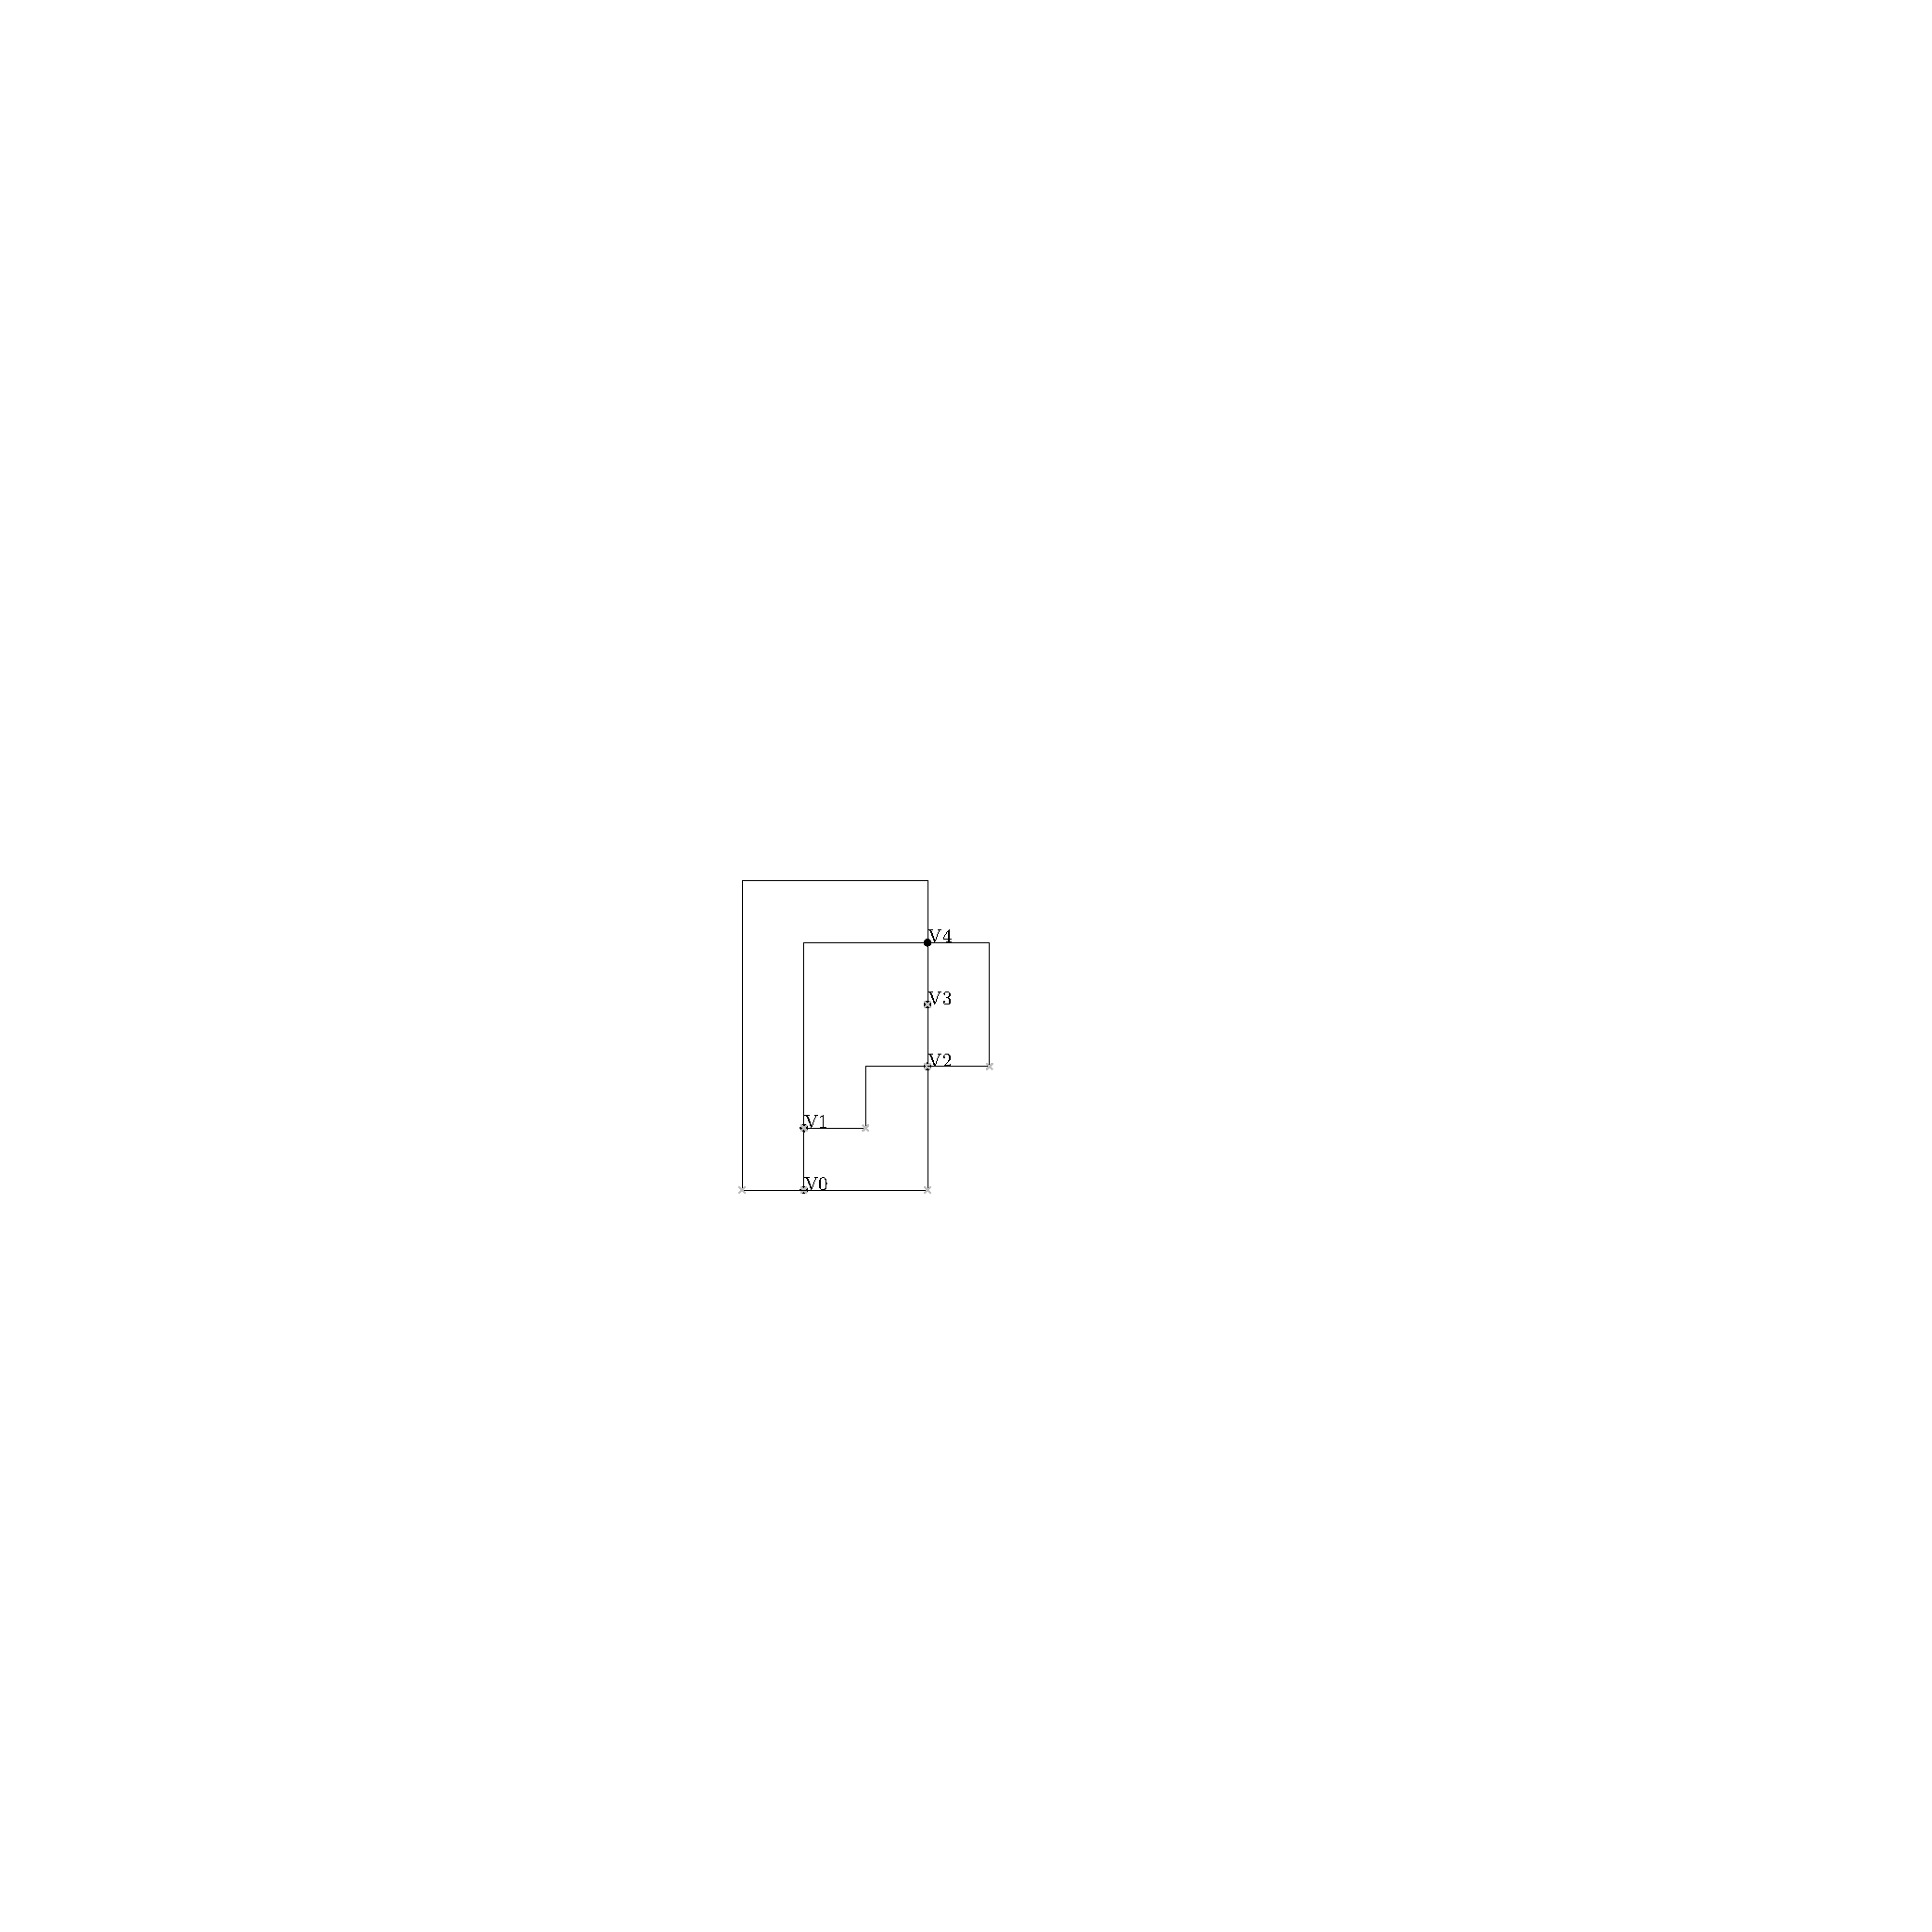
\includegraphics[scale=.7]{exampleA/orthogonalNocompress}
  \label{fig:exampleAorthogonalNocompress}
\end{figure}
\end{column}
\begin{column}{5cm}
\begin{figure}[h]
  \centering
  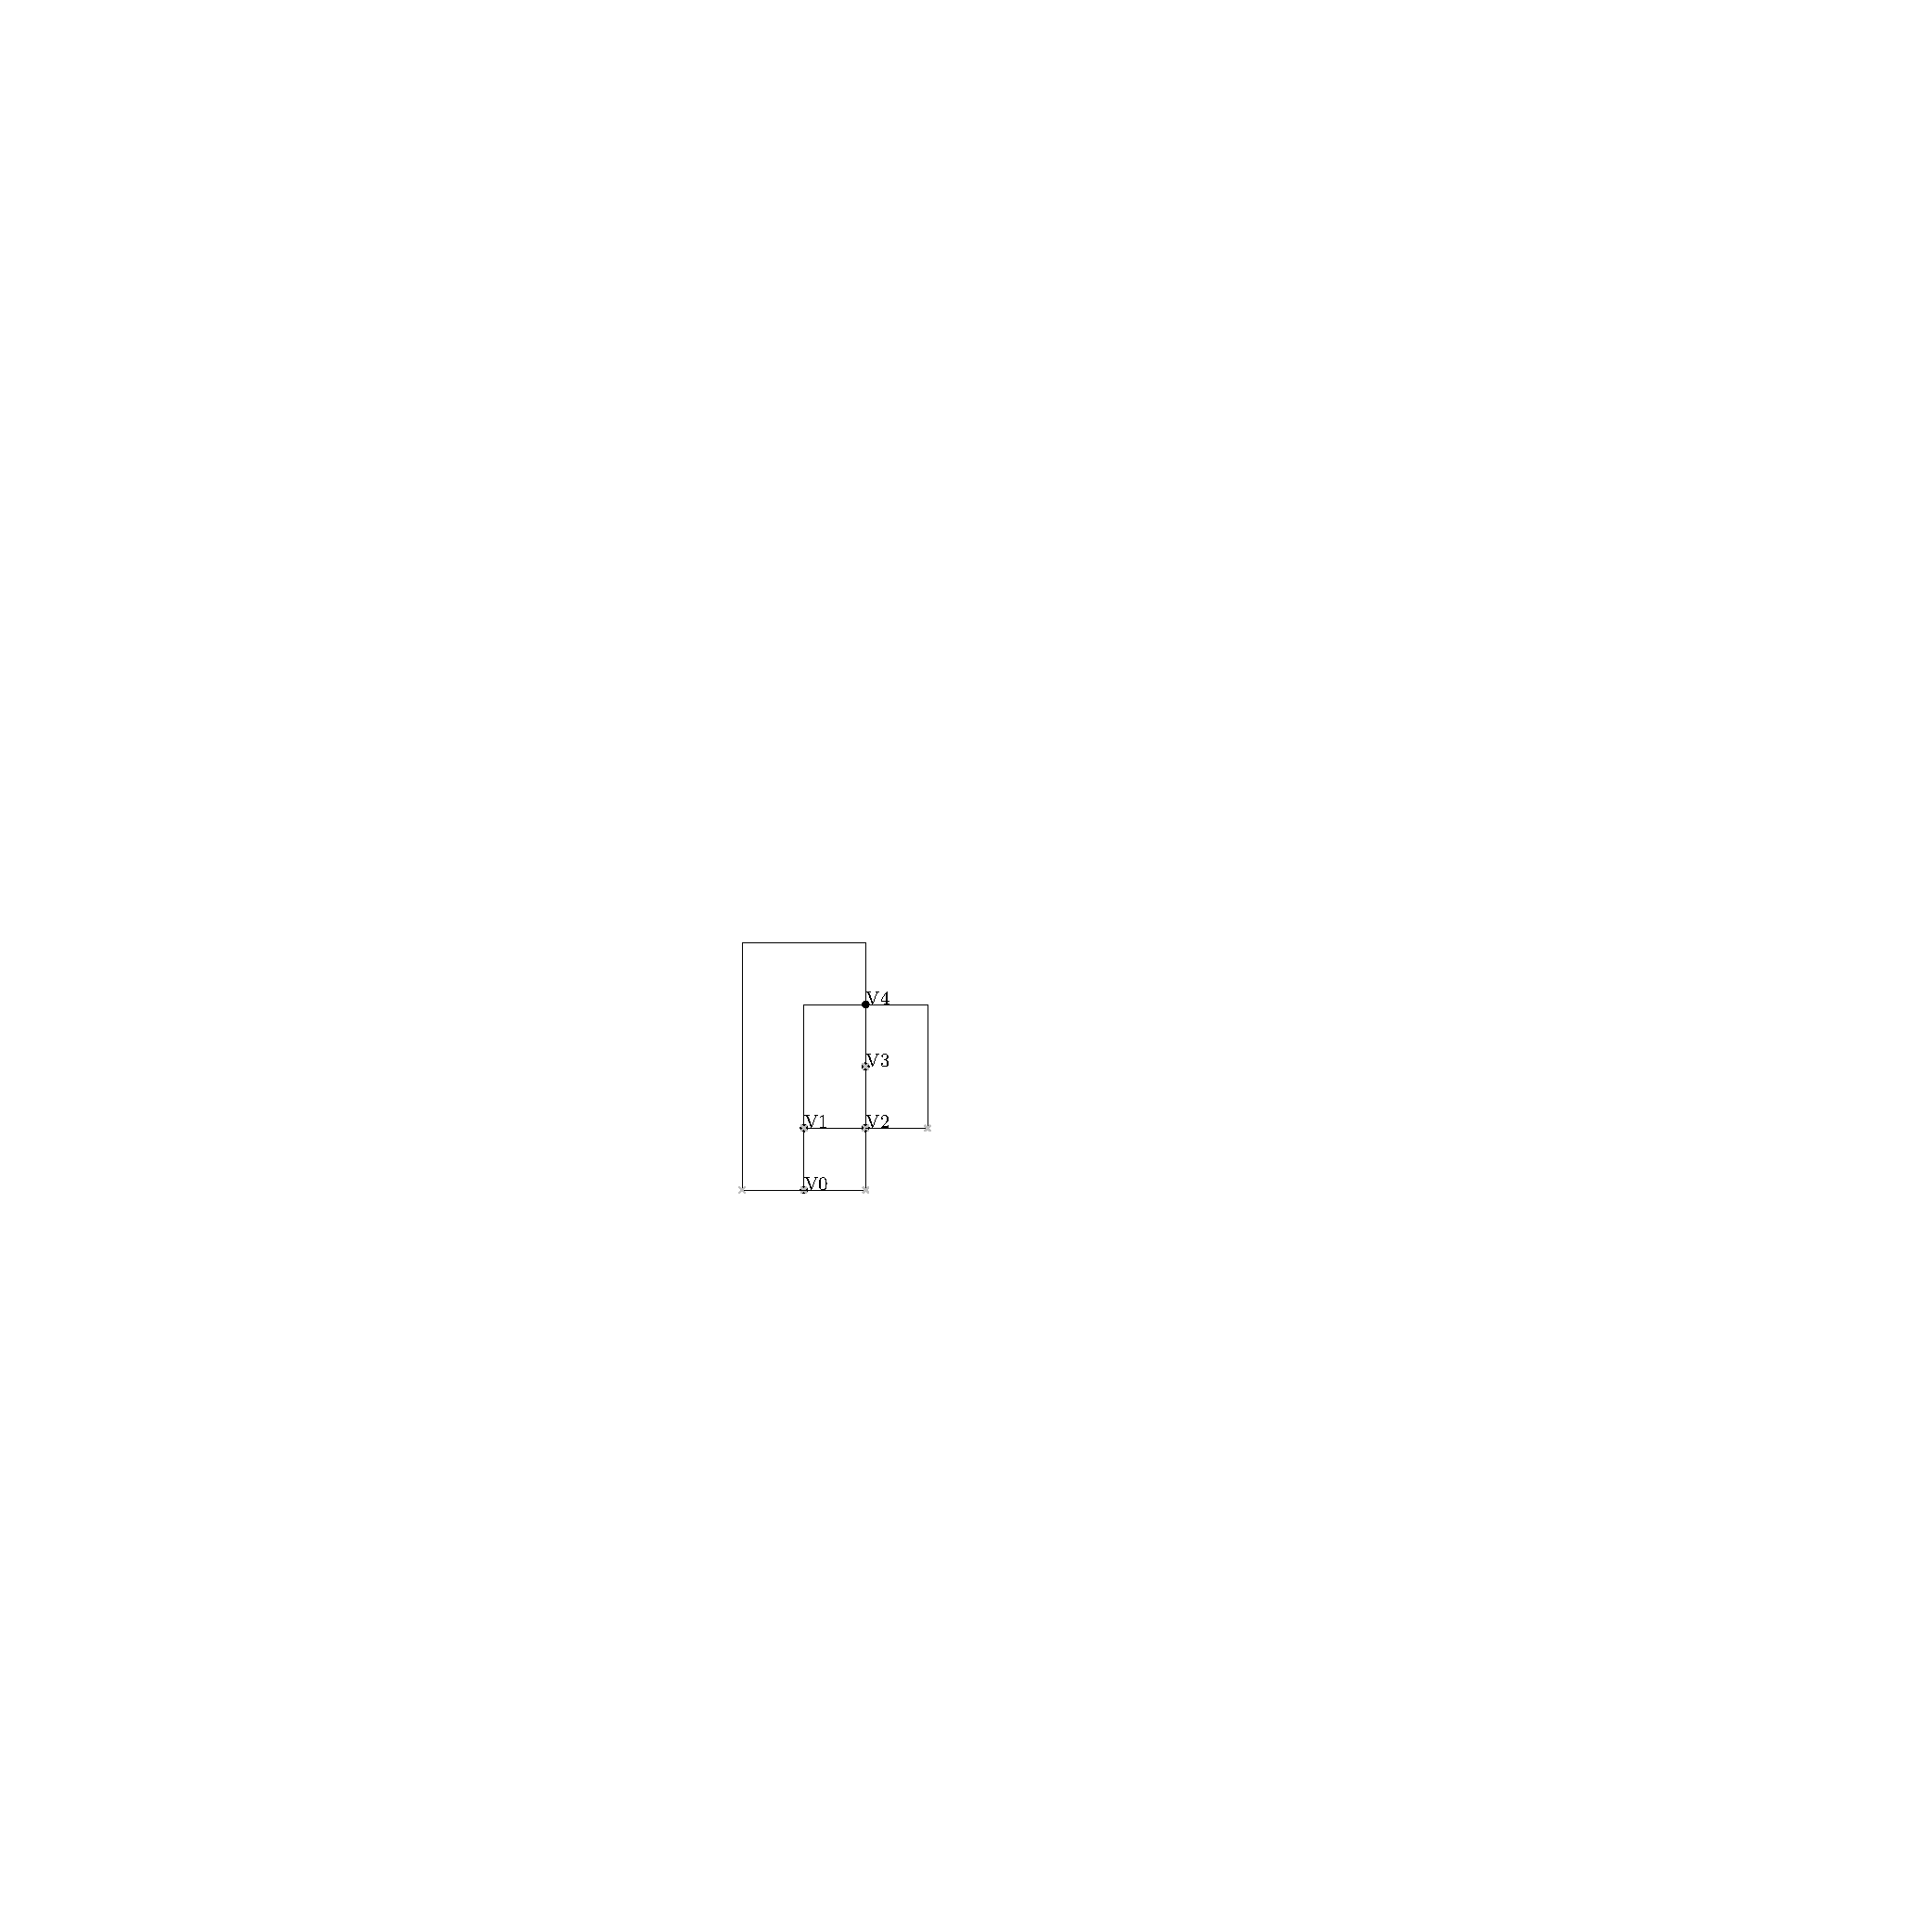
\includegraphics[scale=.7]{exampleA/orthogonalCompress}
  \label{fig:exampleAorthogonalNocompress}
\end{figure}
\end{column}
\end{columns}
\end{frame}

\begin{frame}
  \frametitle{Problem: Neue Überschneidungen}
  \begin{itemize}[<+->]
    \item Abrunden führt zu Überschneidungen
    \item Kreisbögen so, dass Kanten nur zwei Segmente haben
    \item Graph auseinander ziehen, Platz schaffen
    \item An horizontalen Segmenten teilen
  \end{itemize}
\end{frame}

% TODO: Bilder

\begin{frame}
  \frametitle{Wo kann es zu Überschneidungen kommen?}
  \begin{itemize}[<+->]
    \item Innen an C- und L"~Kanten: Plateaus nach oben schieben
    \item Außen an C"~Kanten: Graph auseinander ziehen
    \item Alle C- und L"~Kanten müssen horizontales Segment haben
  \end{itemize}
\end{frame}


\begin{frame}
  \frametitle{Kollisionen mit C"~Kante vermeiden}
 \begin{figure}[h]
        \centering
            {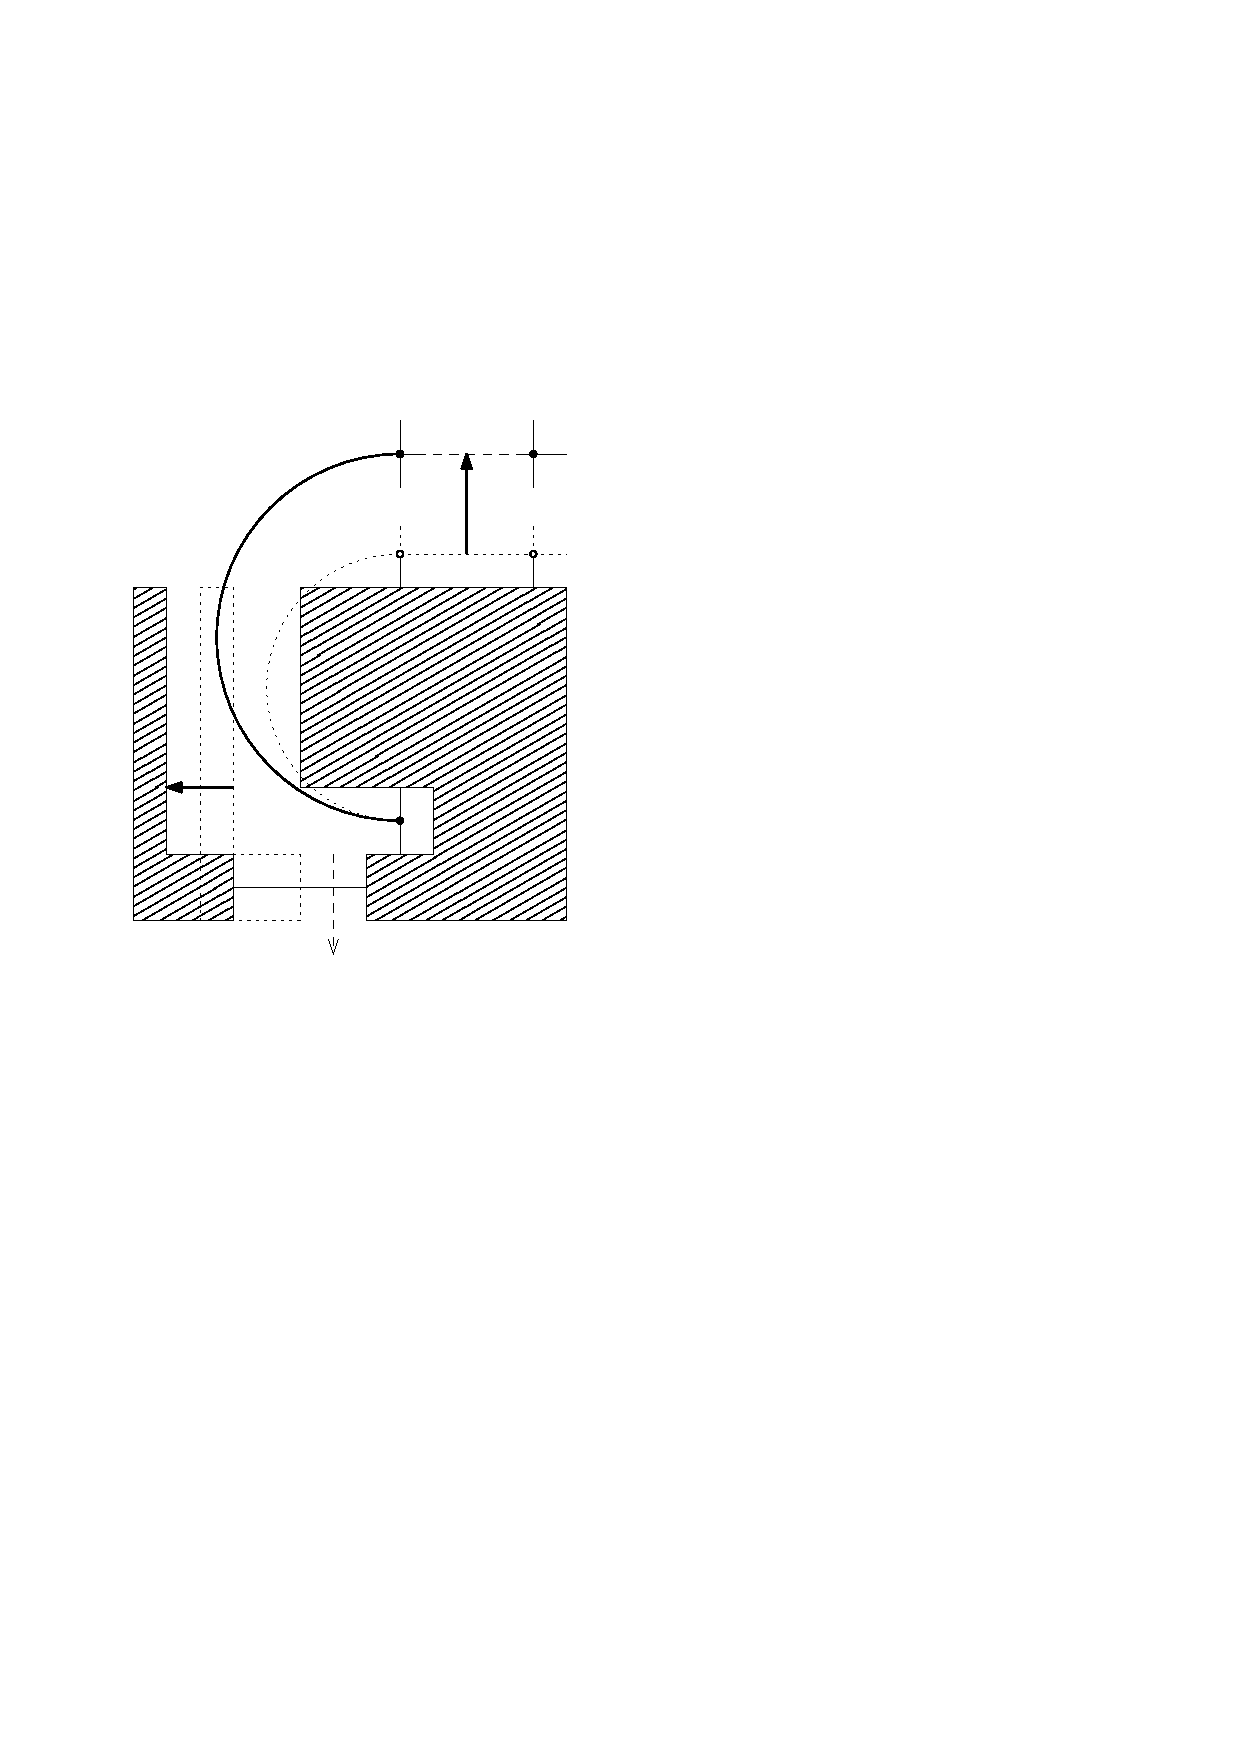
\includegraphics[width=.5\textwidth]{accomodate_C_edge}}
        \caption{Maßnahmen zur Vermeidung von Kollisionen mit C"~Kante.}
\end{figure}
\end{frame}


\begin{frame}
  \frametitle{Schnitte durch Graphen finden}
  \begin{itemize}[<+->]
    \item Immer an einem Knoten, in einem Quadranten
    \item C"~, I"~~und L"~Kanten an horizontalen Segmenten durchqueren
    \item Kein vertikales Segment durchqueren
    \item Kante folgen oder durchschneiden
  \end{itemize}
\end{frame}

% TODO: fig: cutfinding?

% TODO: zeichenen der g/o kanten (nur mit ports u. lage!)?

% TODO: erkennung von überschenidungen g/o kanten?

% TODO: (kompletter beispieldurchlauf)


\begin{frame}[b]
  \frametitle{Beispieldurchlauf}
  \includegraphics<1>[scale=.55,page=1]{walkthrough}
  \includegraphics<2>[scale=.55,page=2]{walkthrough}
  \includegraphics<3>[scale=.55,page=3]{walkthrough}
  \includegraphics<4>[scale=.55,page=4]{walkthrough}
  \includegraphics<5>[scale=.55,page=5]{walkthrough}
  \includegraphics<6>[scale=.55,page=6]{walkthrough}
  \includegraphics<7>[scale=.55,page=7]{walkthrough}
  \includegraphics<8>[scale=.55,page=8]{walkthrough}
  \includegraphics<9>[scale=.55,page=9]{walkthrough}
  \includegraphics<10>[scale=.55,page=10]{walkthrough}
  \includegraphics<11>[scale=.55,page=11]{walkthrough}
  \includegraphics<12>[scale=.55,page=12]{walkthrough}
  \includegraphics<13>[scale=.55,page=13]{walkthrough}
  \includegraphics<14>[scale=.55,page=14]{walkthrough}
  \includegraphics<15>[scale=.55,page=15]{walkthrough}
  \includegraphics<16>[scale=.55,page=16]{walkthrough}
  \includegraphics<17>[scale=.55,page=17]{walkthrough}
  \includegraphics<18>[scale=.55,page=18]{walkthrough}
  \includegraphics<19>[scale=.55,page=19]{walkthrough}
  \includegraphics<20>[scale=.55,page=20]{walkthrough}
\end{frame}


\section{Verbesserungen}
\frame{\tableofcontents[currentsection]}


\begin{frame}
  \frametitle{Eigene Anpassungen für die Implementierung}
  \begin{itemize}[<+->]
    \item Schnitte nur anhand der Ports, statt geometrisch
    \item Zeichnen von glatt"=orthogonalen Kanten
    \item Finden von Überschneidungen von Kreissegmenten und Linien
  \end{itemize}
Optimierungen:
  \begin{itemize}[<+->]
    \item Plateaus mit gleicher Höhe
    \item Korrektur der Steigung der Kanten nur wenn nötig
    \item Keine G"~Kanten
  \end{itemize}
\end{frame}

\begin{frame}
  \frametitle{ Plateaus mit gleicher Höhe }

\begin{columns}[b]
\begin{column}{5cm}
\begin{figure}[h]
  \centering
  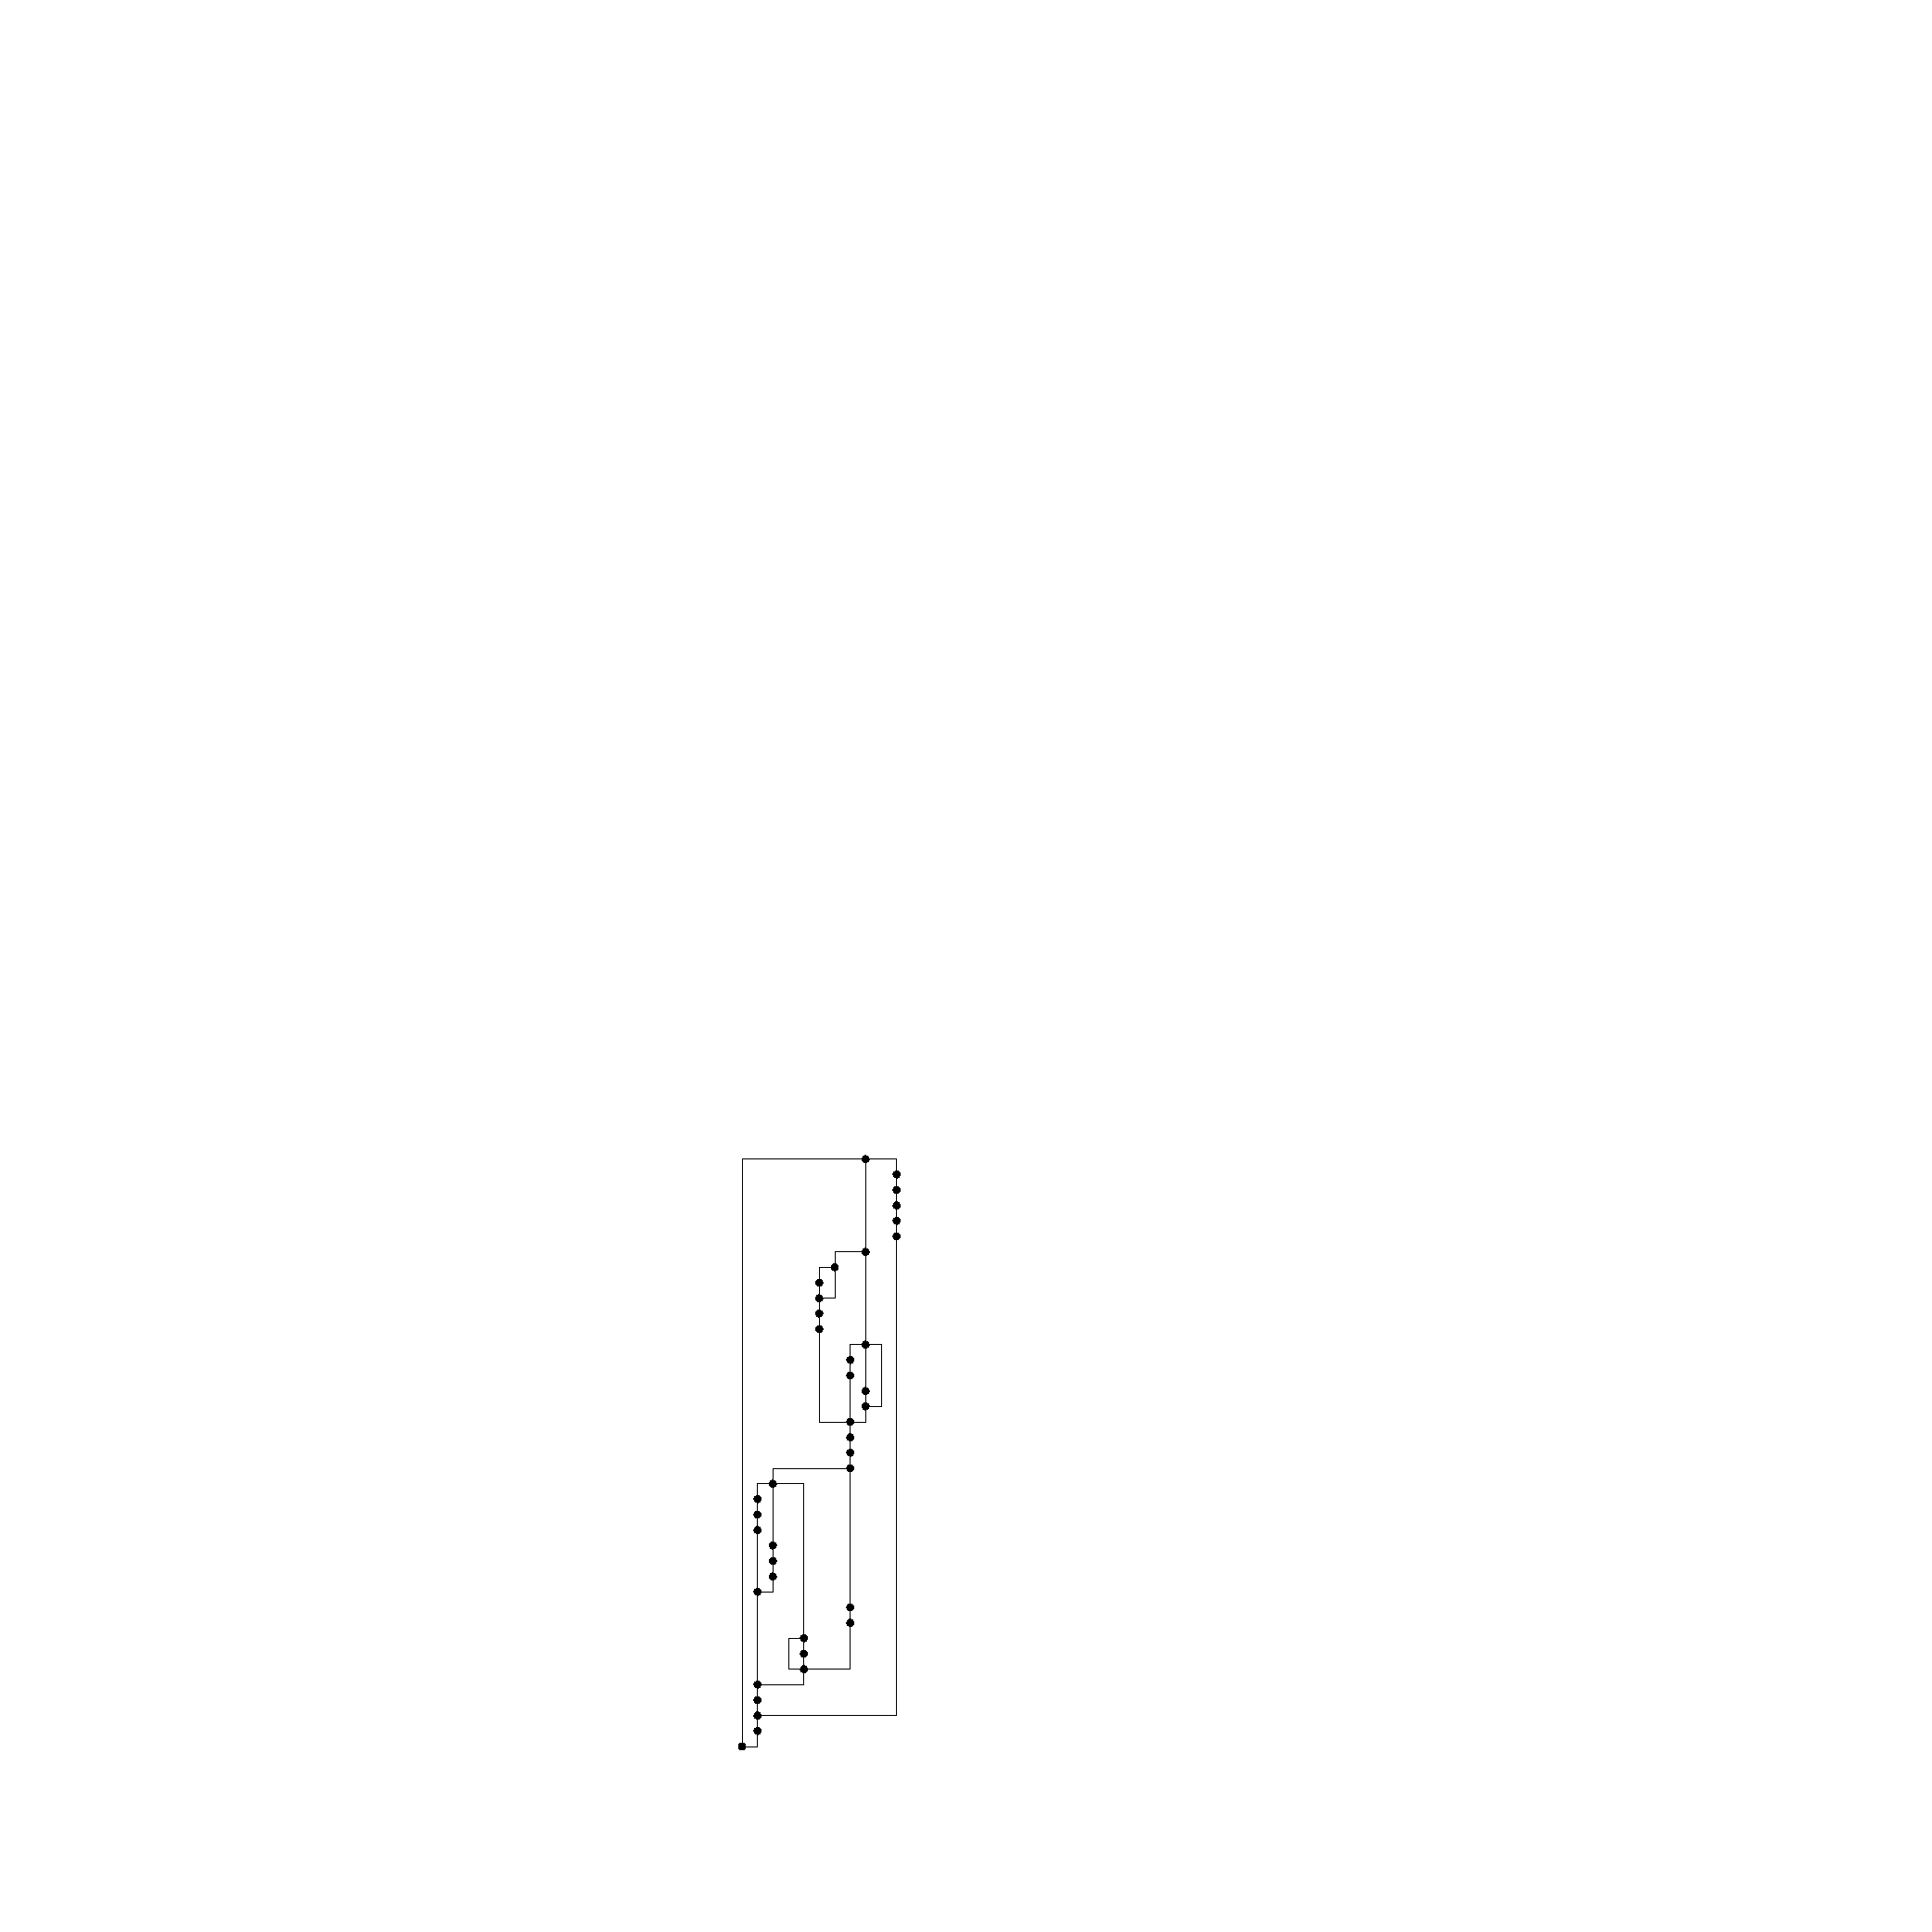
\includegraphics[scale=.6]{compressableGraph/isUncompressed}
  \caption{Ohne Komprimierung Höhe 38}
  \label{fig:exampleAsmoothComplex}
\end{figure}
\end{column}
\begin{column}{5cm}
\begin{figure}[h]
  \centering
  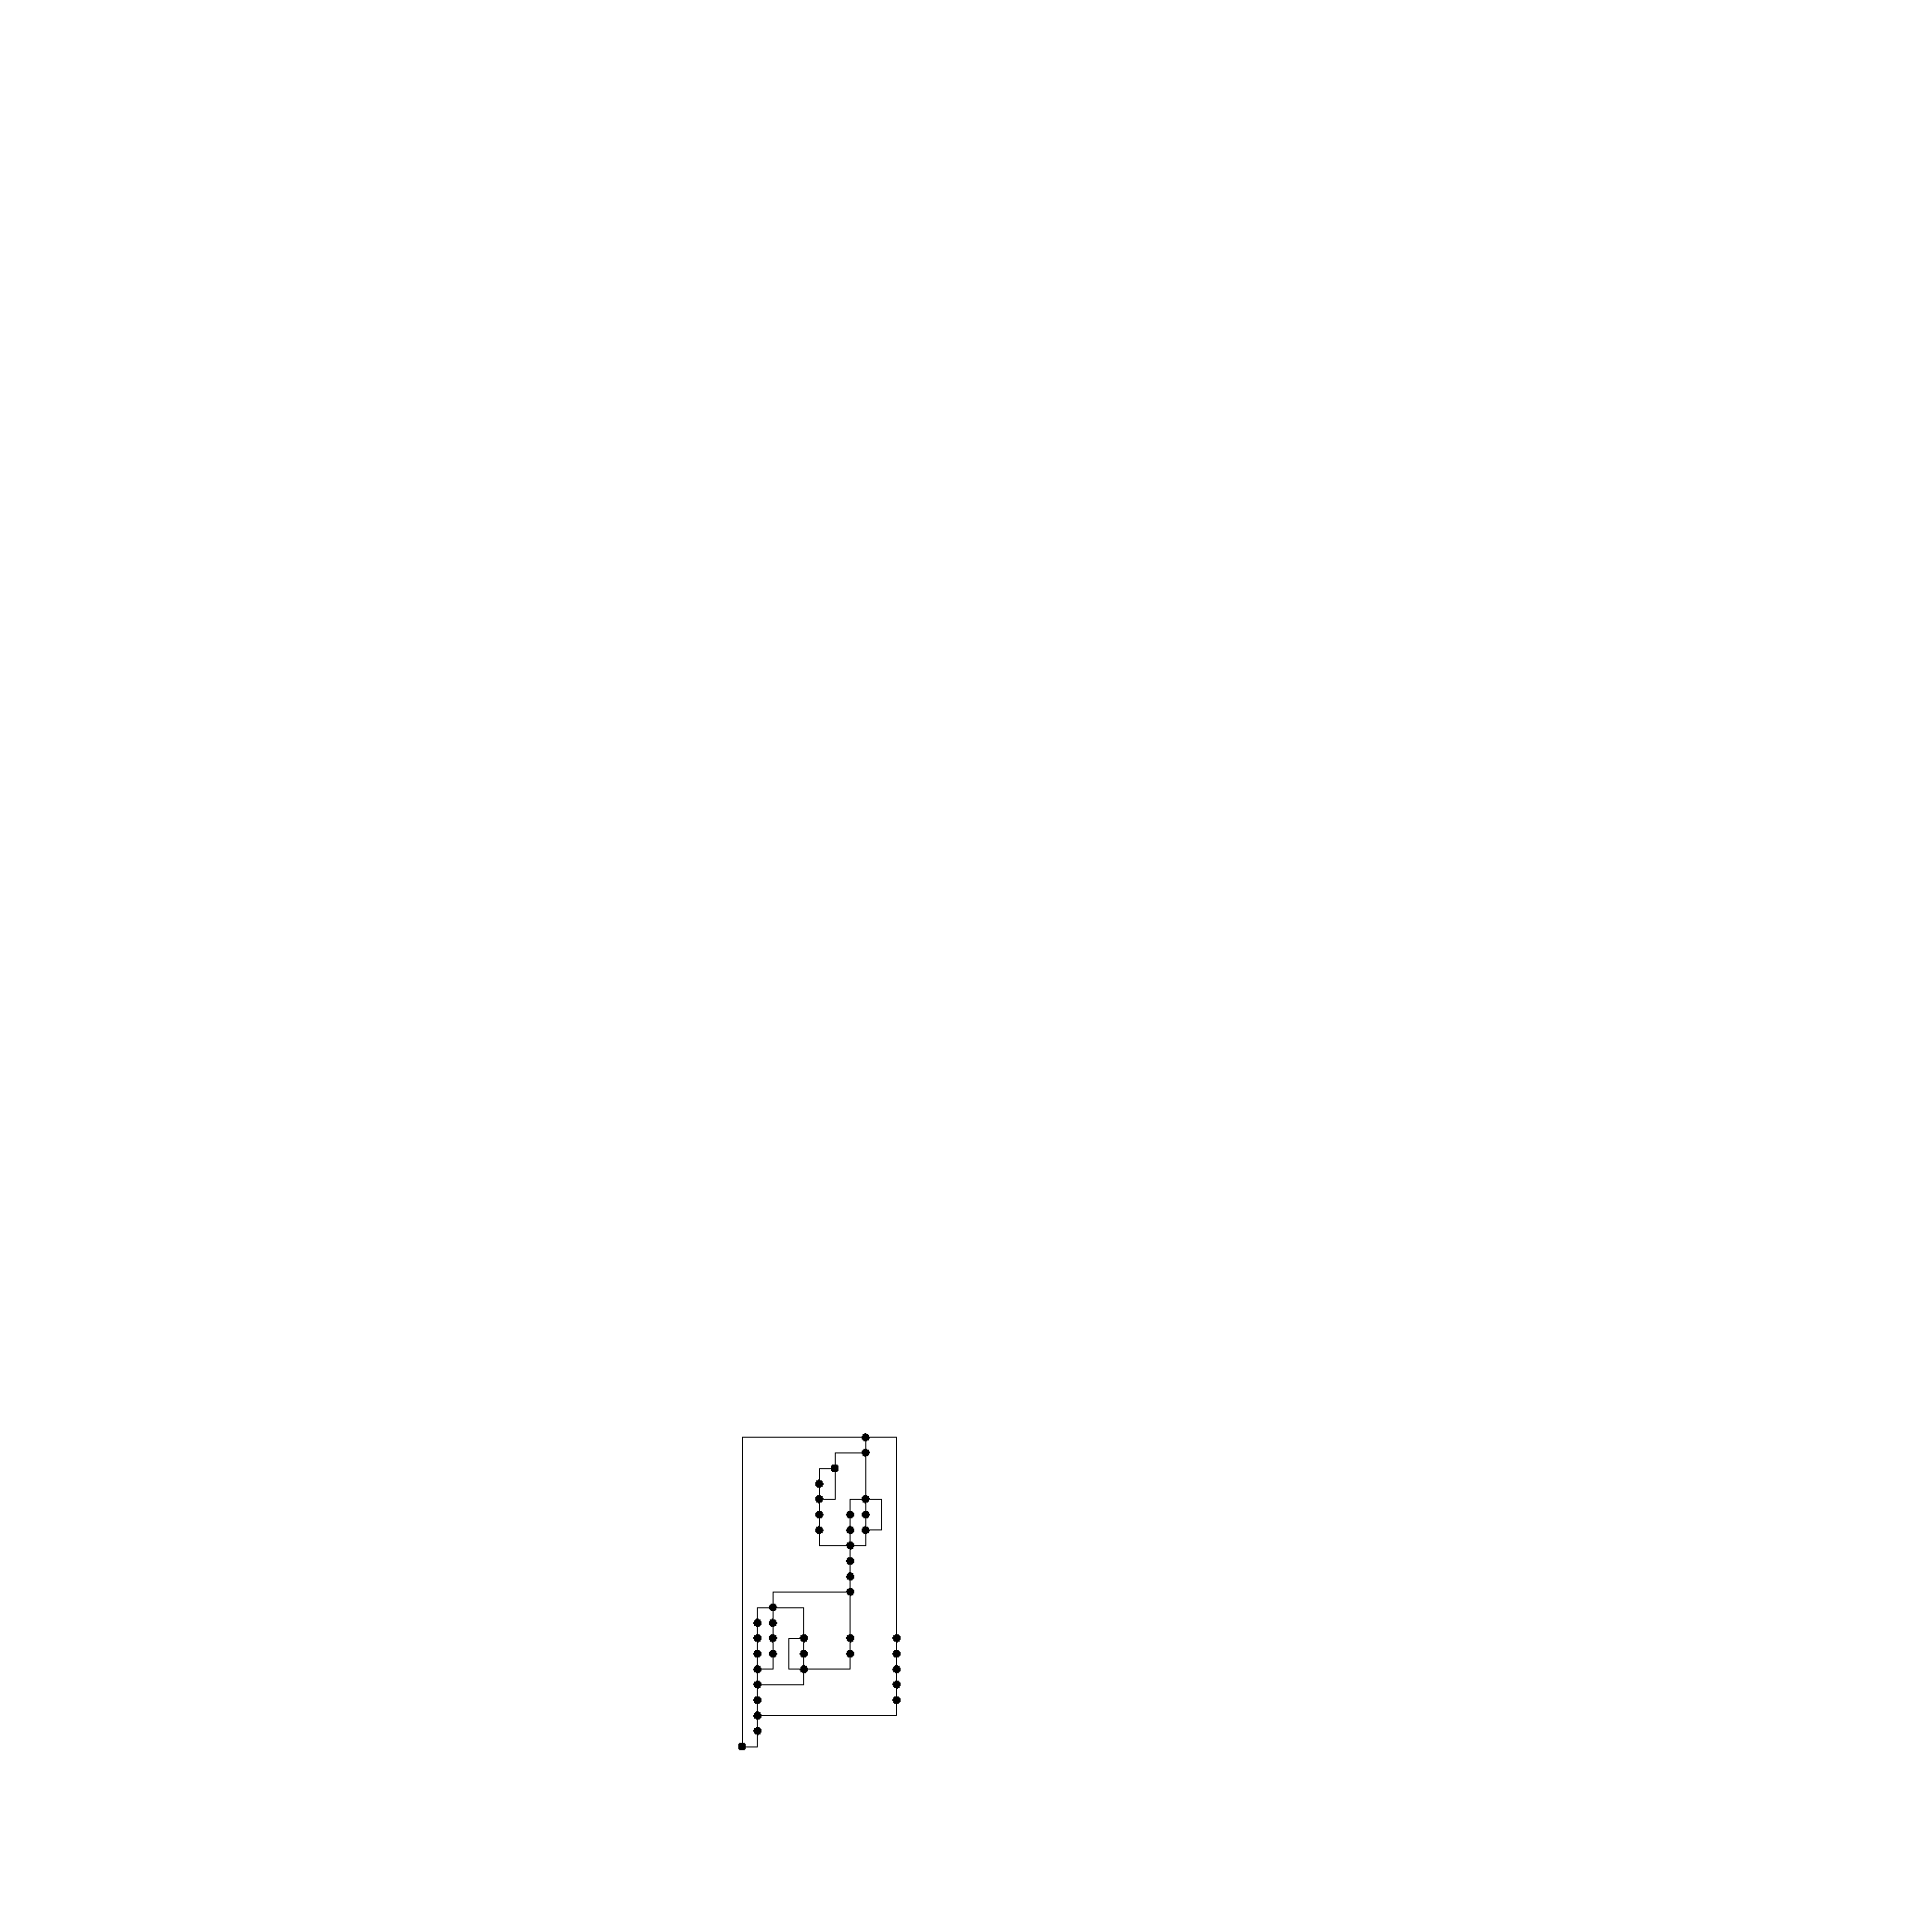
\includegraphics[scale=.6]{compressableGraph/isCompressed}
  \caption{Mit Komprimierung Höhe 20}
  \label{fig:exampleAsmoothSimple}
\end{figure}
\end{column}
\end{columns}
\end{frame}

\begin{frame}
  \frametitle{ Korrektur der Steigung der Kanten nur wenn nötig}
\begin{figure}[h]
  \centering
  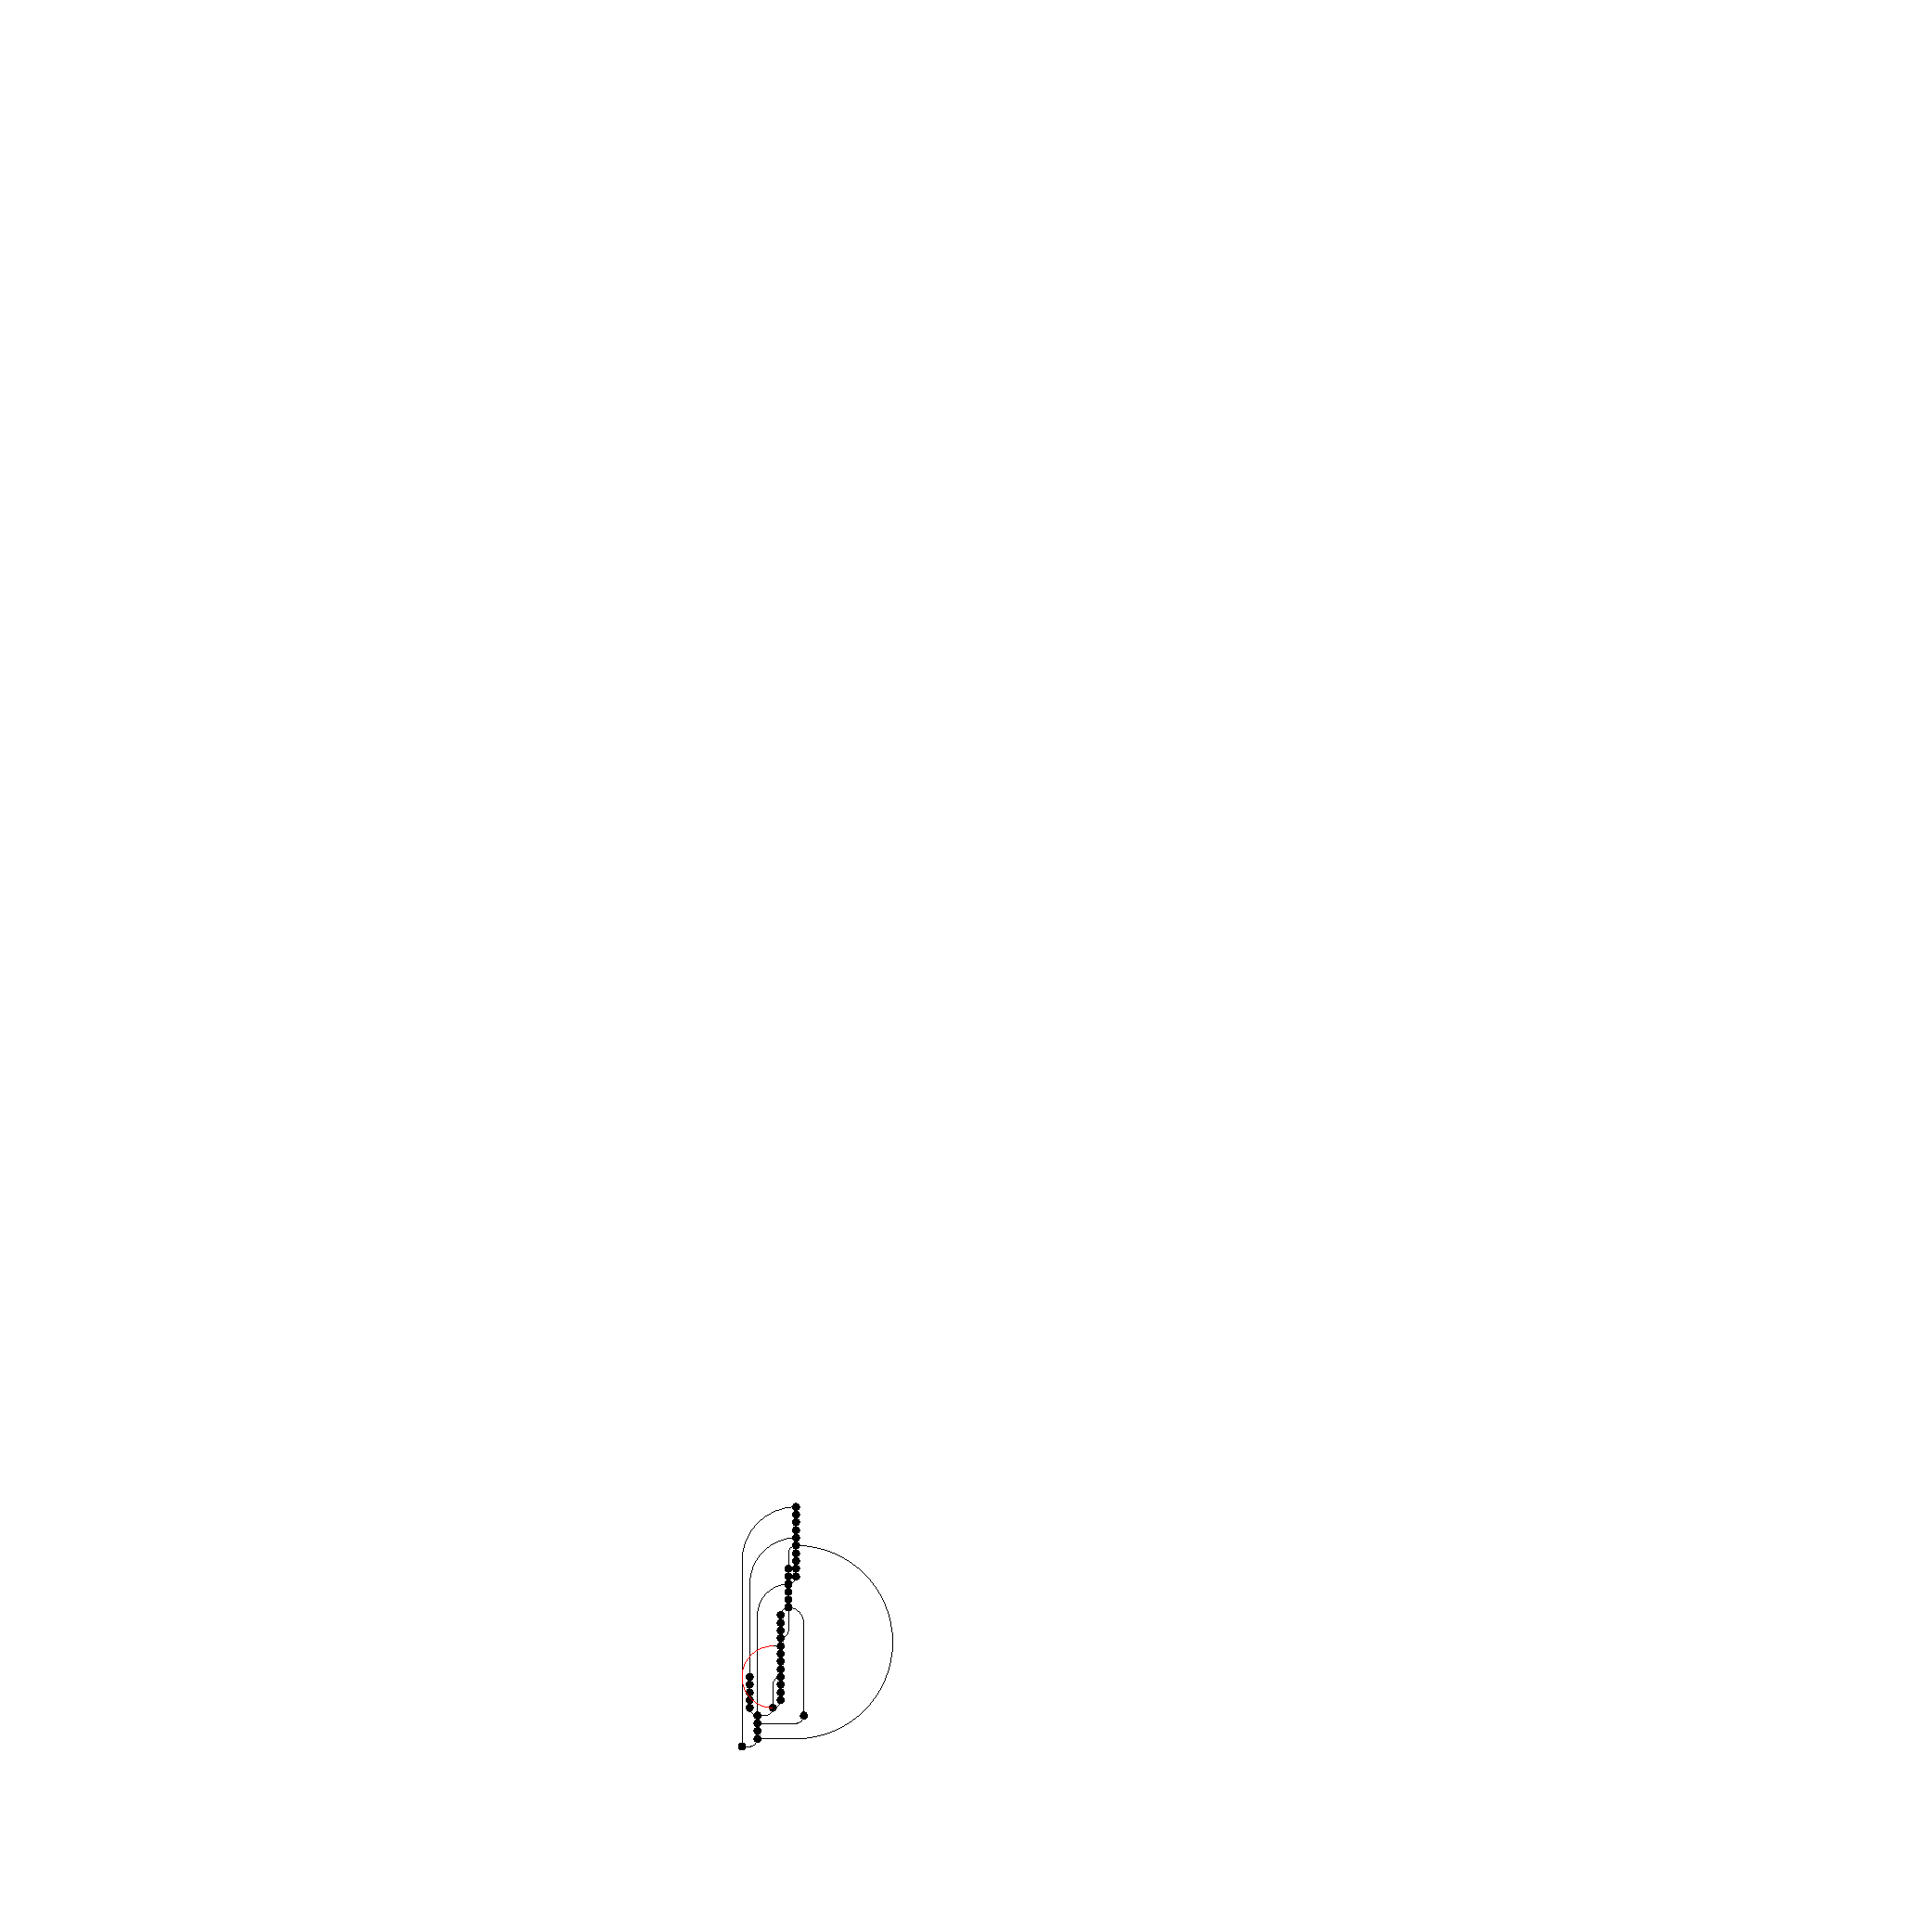
\includegraphics{hugeGraph/isntPlanar}
  \caption{Graph mit Überschneidung}
  \label{fig:exampleAsmoothSimple}
\end{figure}
\end{frame}

\begin{frame}
  \frametitle{ Korrektur der Steigung der Kanten nur wenn nötig}
\begin{figure}[h]
  \centering
  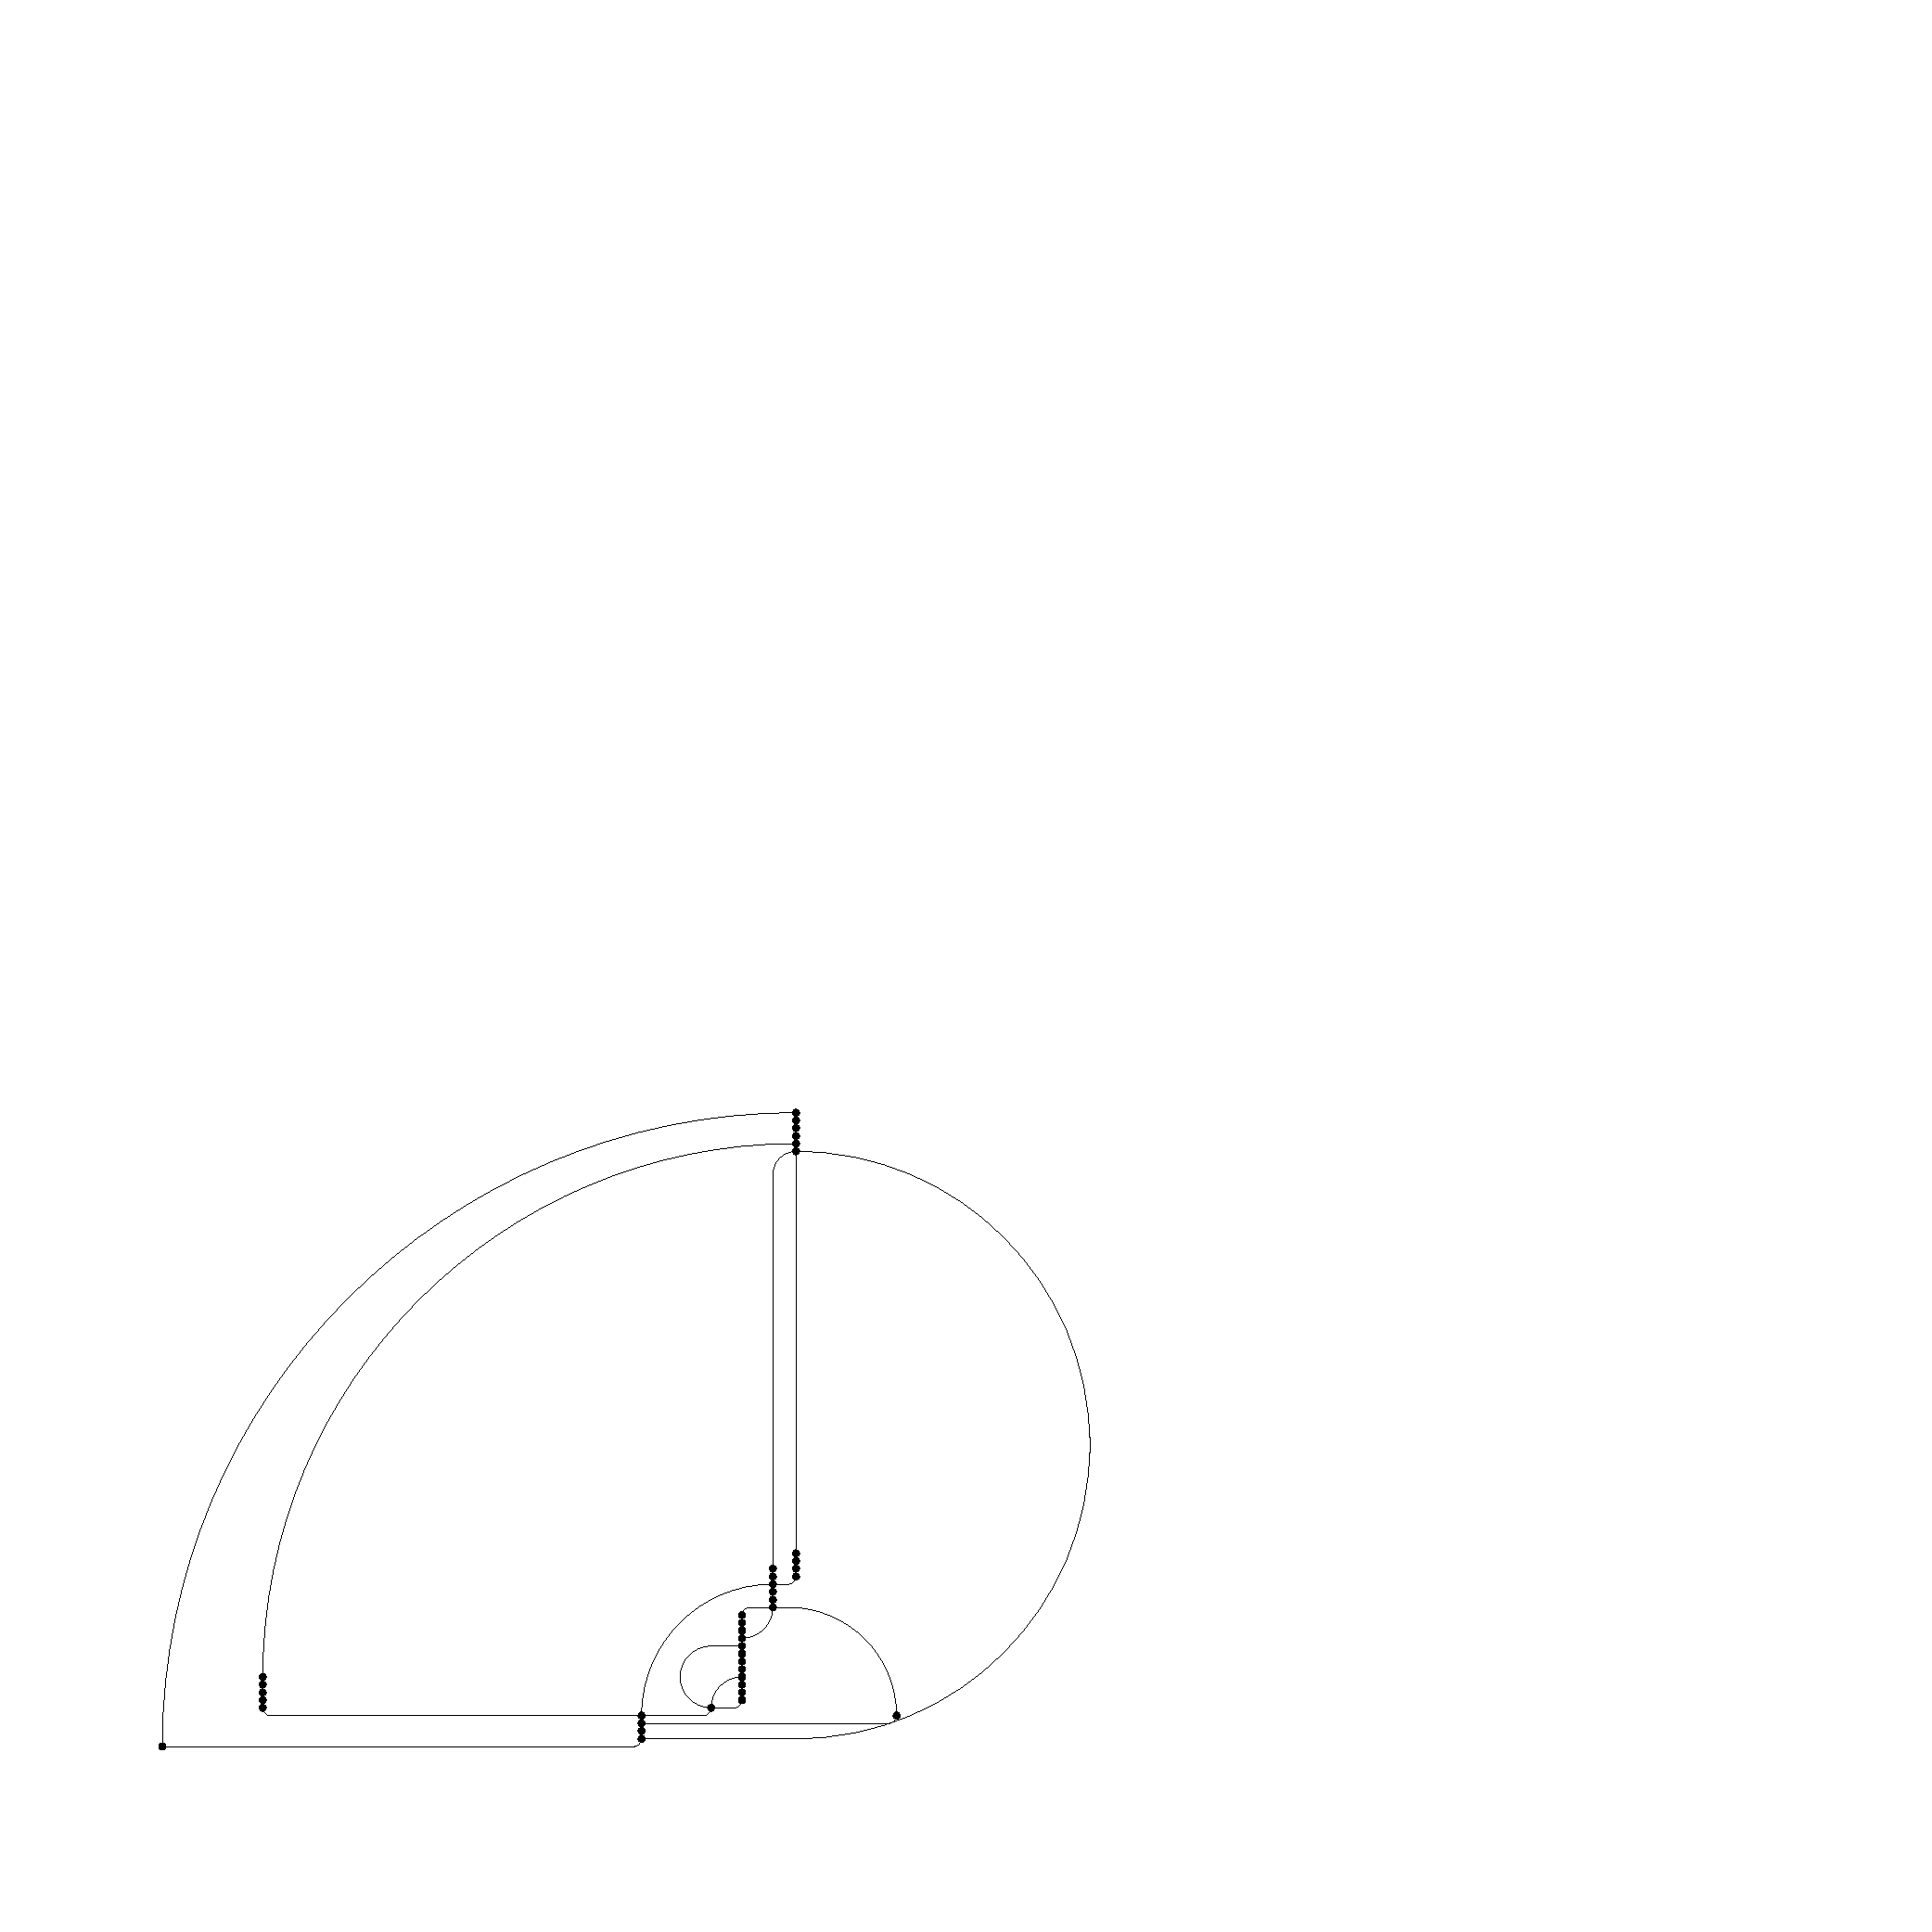
\includegraphics{hugeGraph/isHuge}
  \caption{Graph ohne Überschneidung}
  \label{fig:exampleAsmoothSimple}
\end{figure}
\end{frame}

\begin{frame}
  \frametitle{ Korrektur der Steigung der Kanten nur wenn nötig}
\begin{figure}[h]
  \centering
  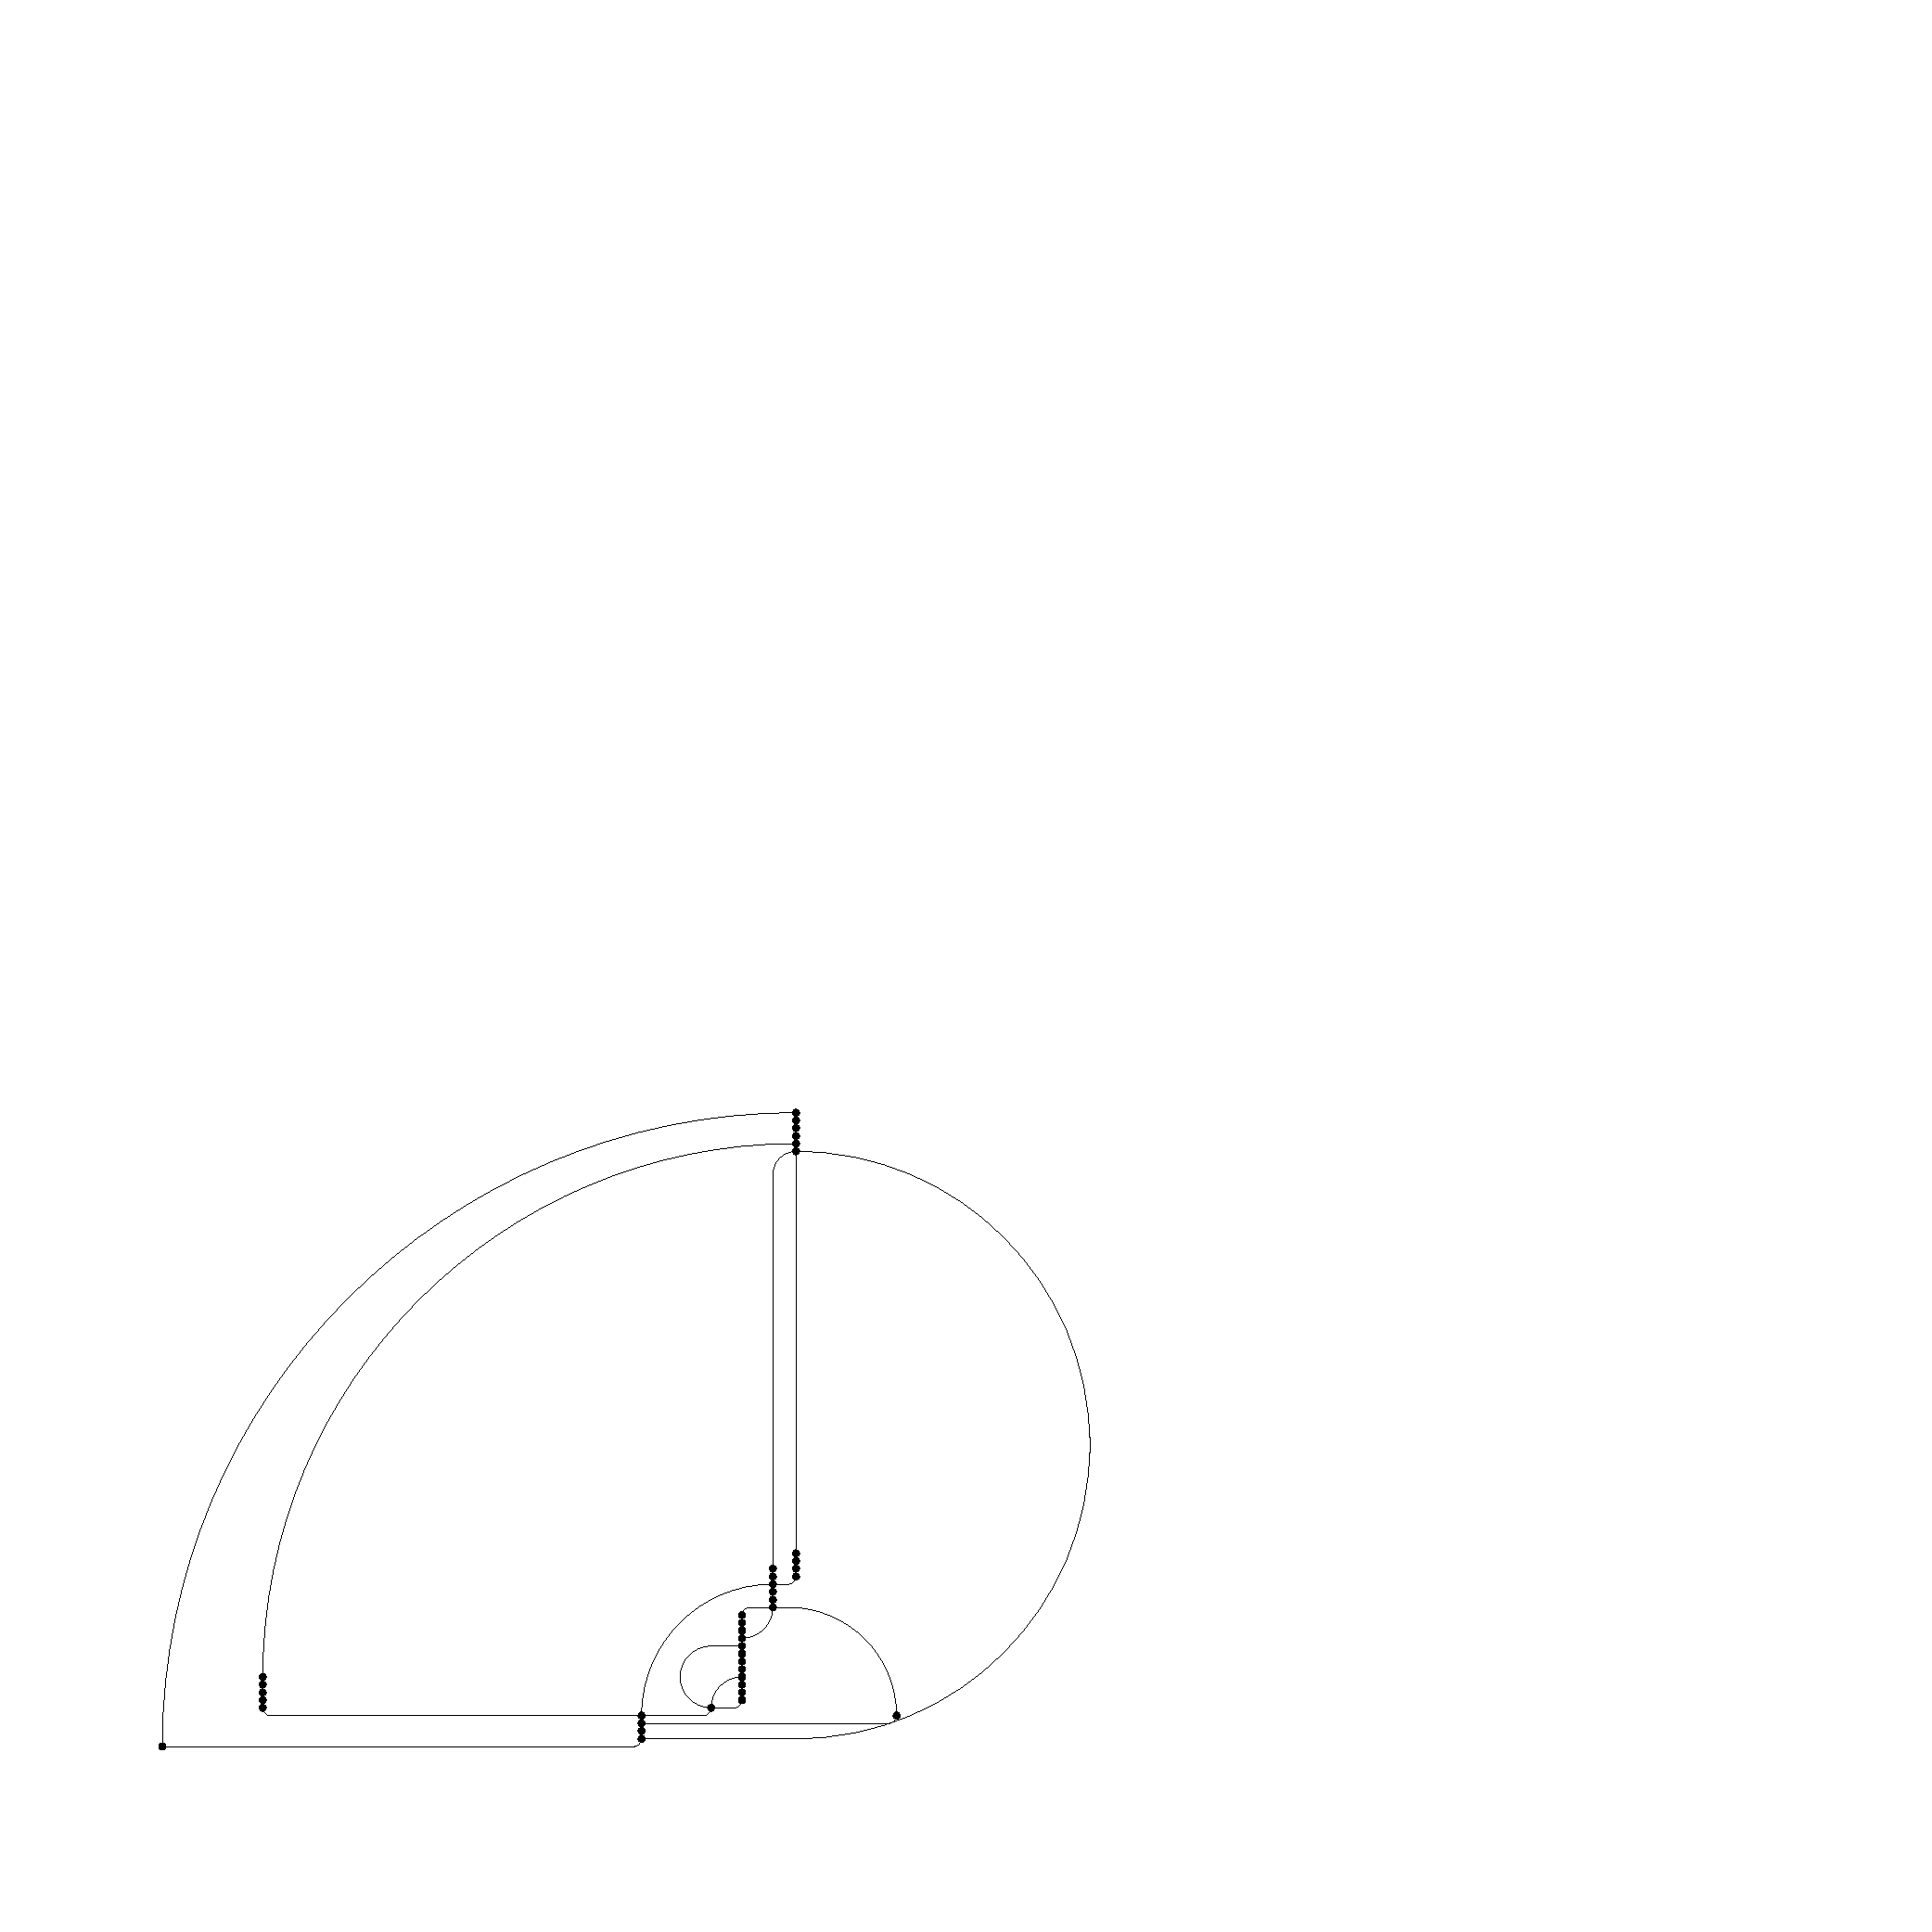
\includegraphics[scale=.4]{hugeGraph/isHuge}
  \caption{Graph ohne Überschneidung (40\%)}
  \label{fig:exampleAsmoothSimple}
\end{figure}
\end{frame}

\begin{frame}
  \frametitle{ Korrektur der Steigung der Kanten nur wenn nötig}
\begin{figure}[h]
  \centering
  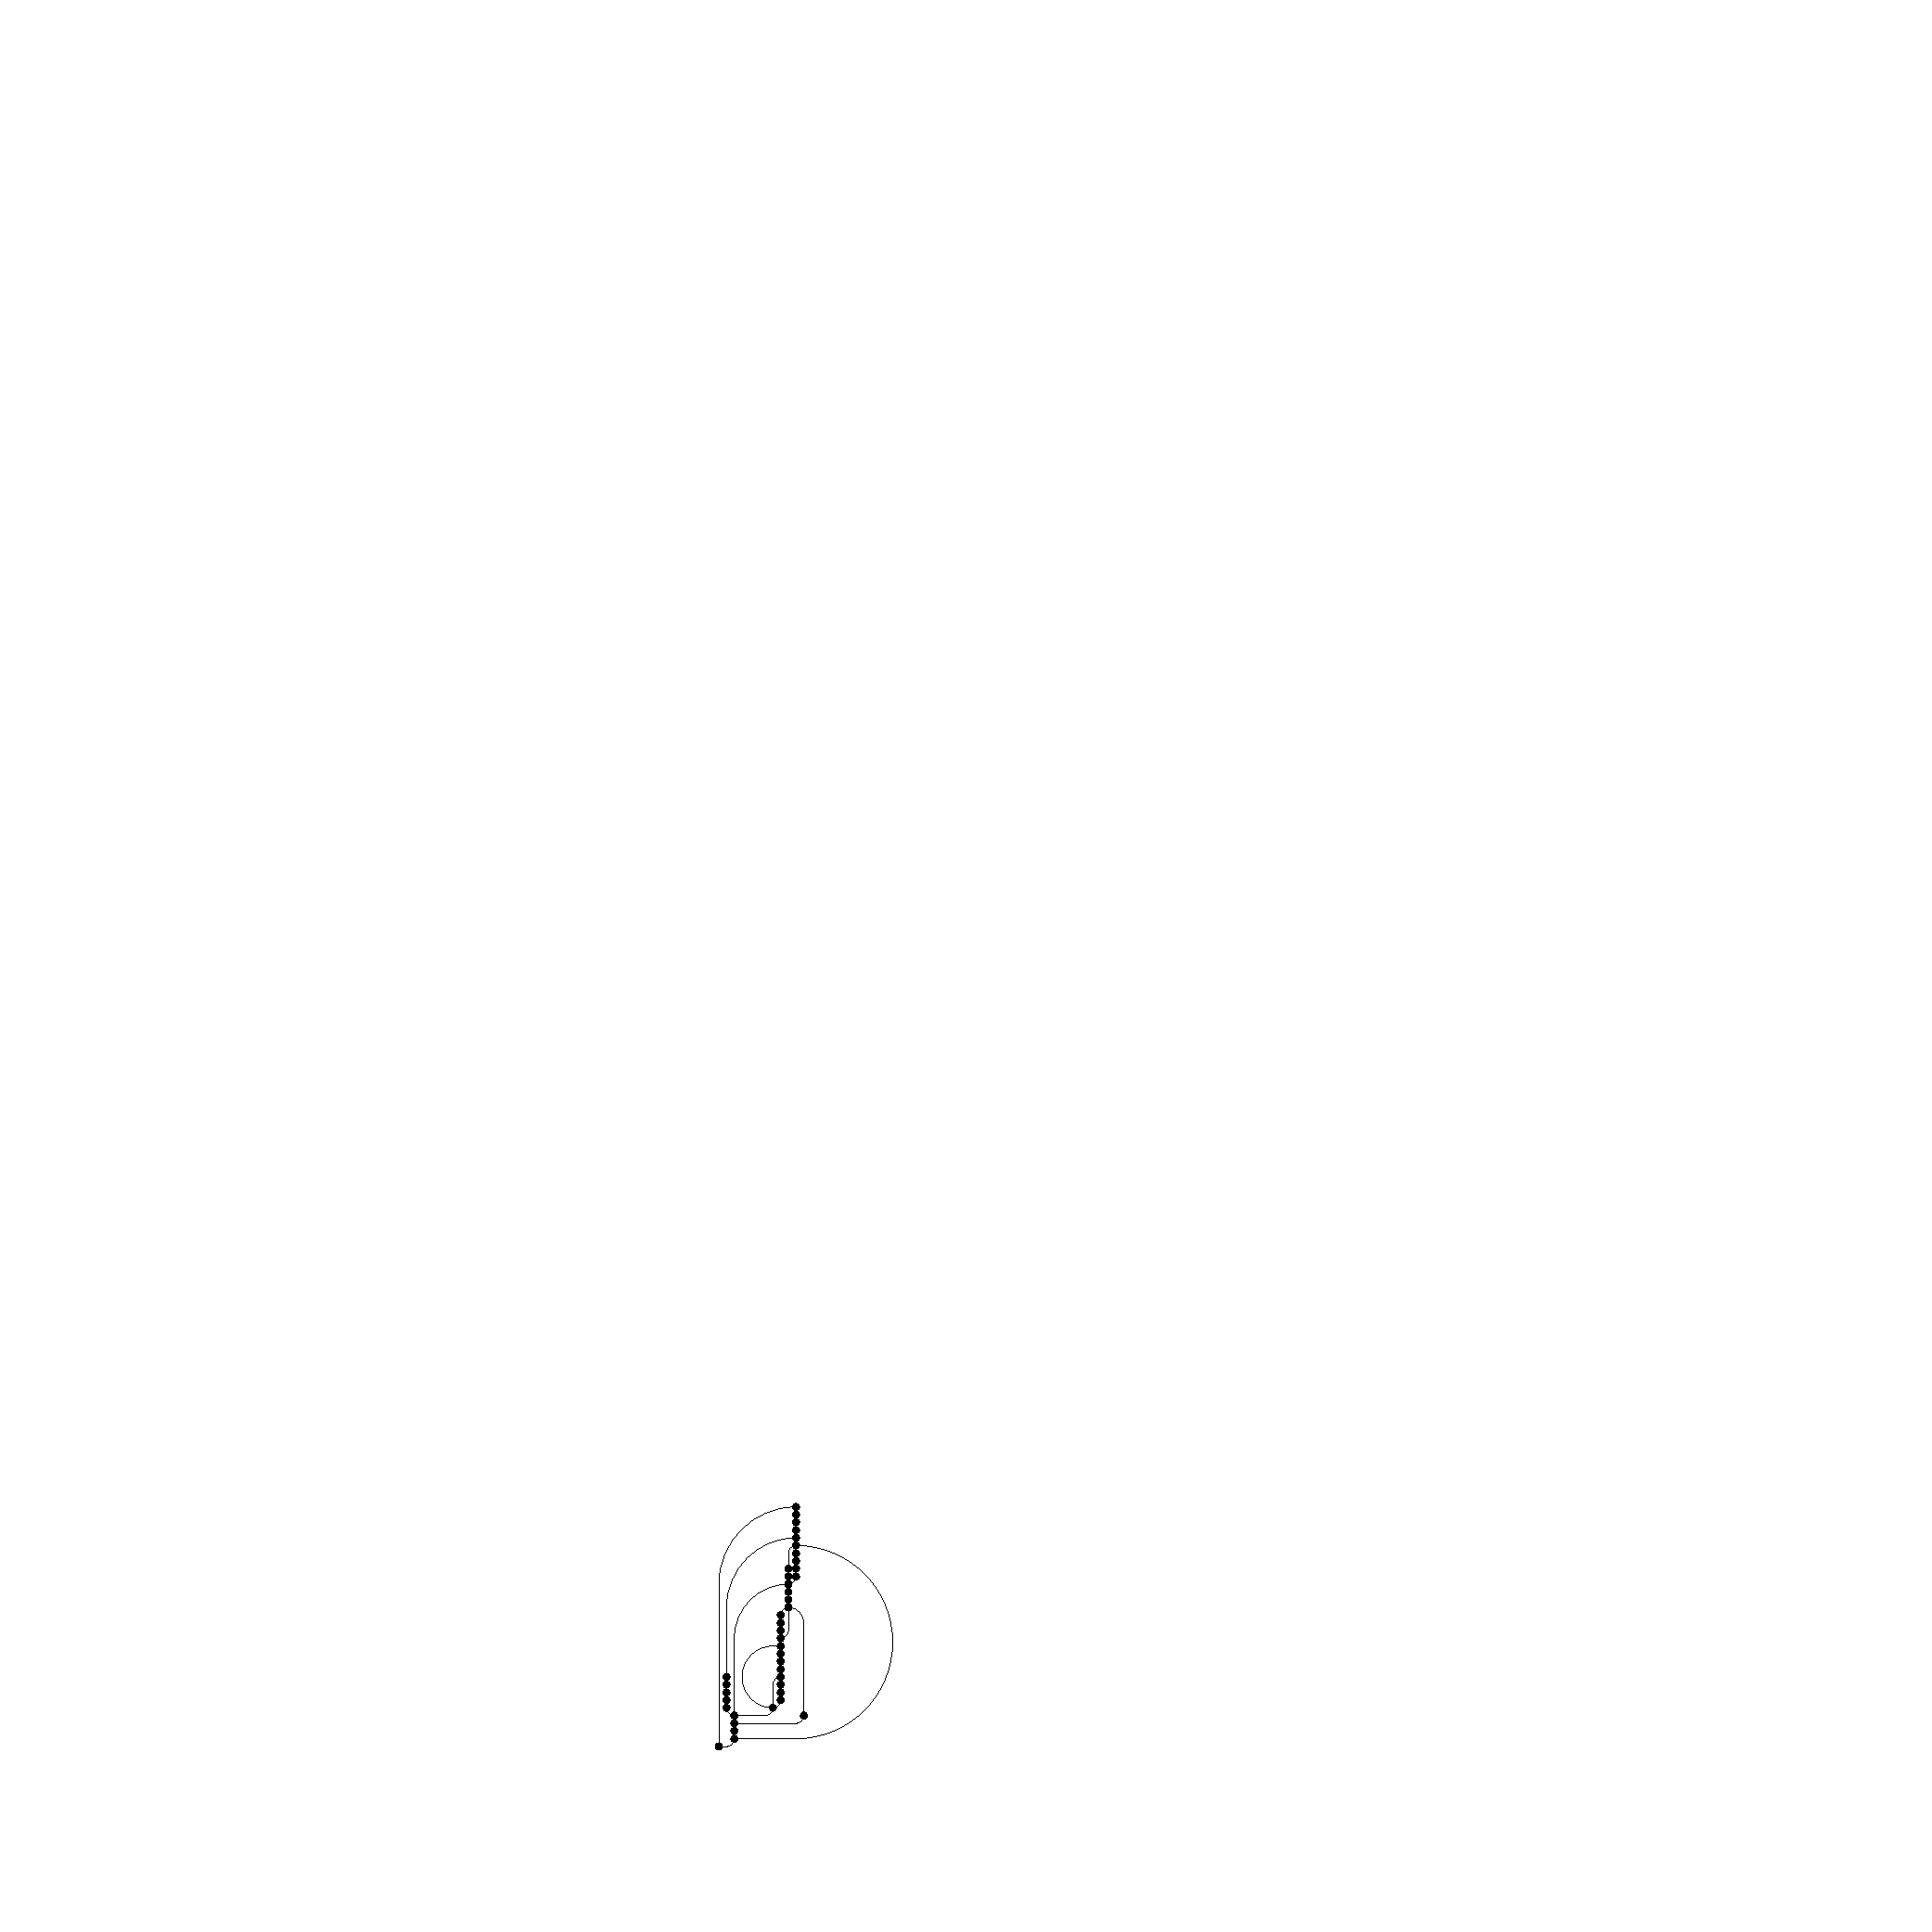
\includegraphics[scale=.4]{hugeGraph/isSmaller}
  \caption{ Korrektur der Steigung ausgesetzt (40\%)}
  \label{fig:exampleAsmoothSimple}
\end{figure}
\end{frame}

\begin{frame}
  \frametitle{ Korrektur der Steigung der Kanten nur wenn nötig}
\begin{figure}[h]
  \centering
  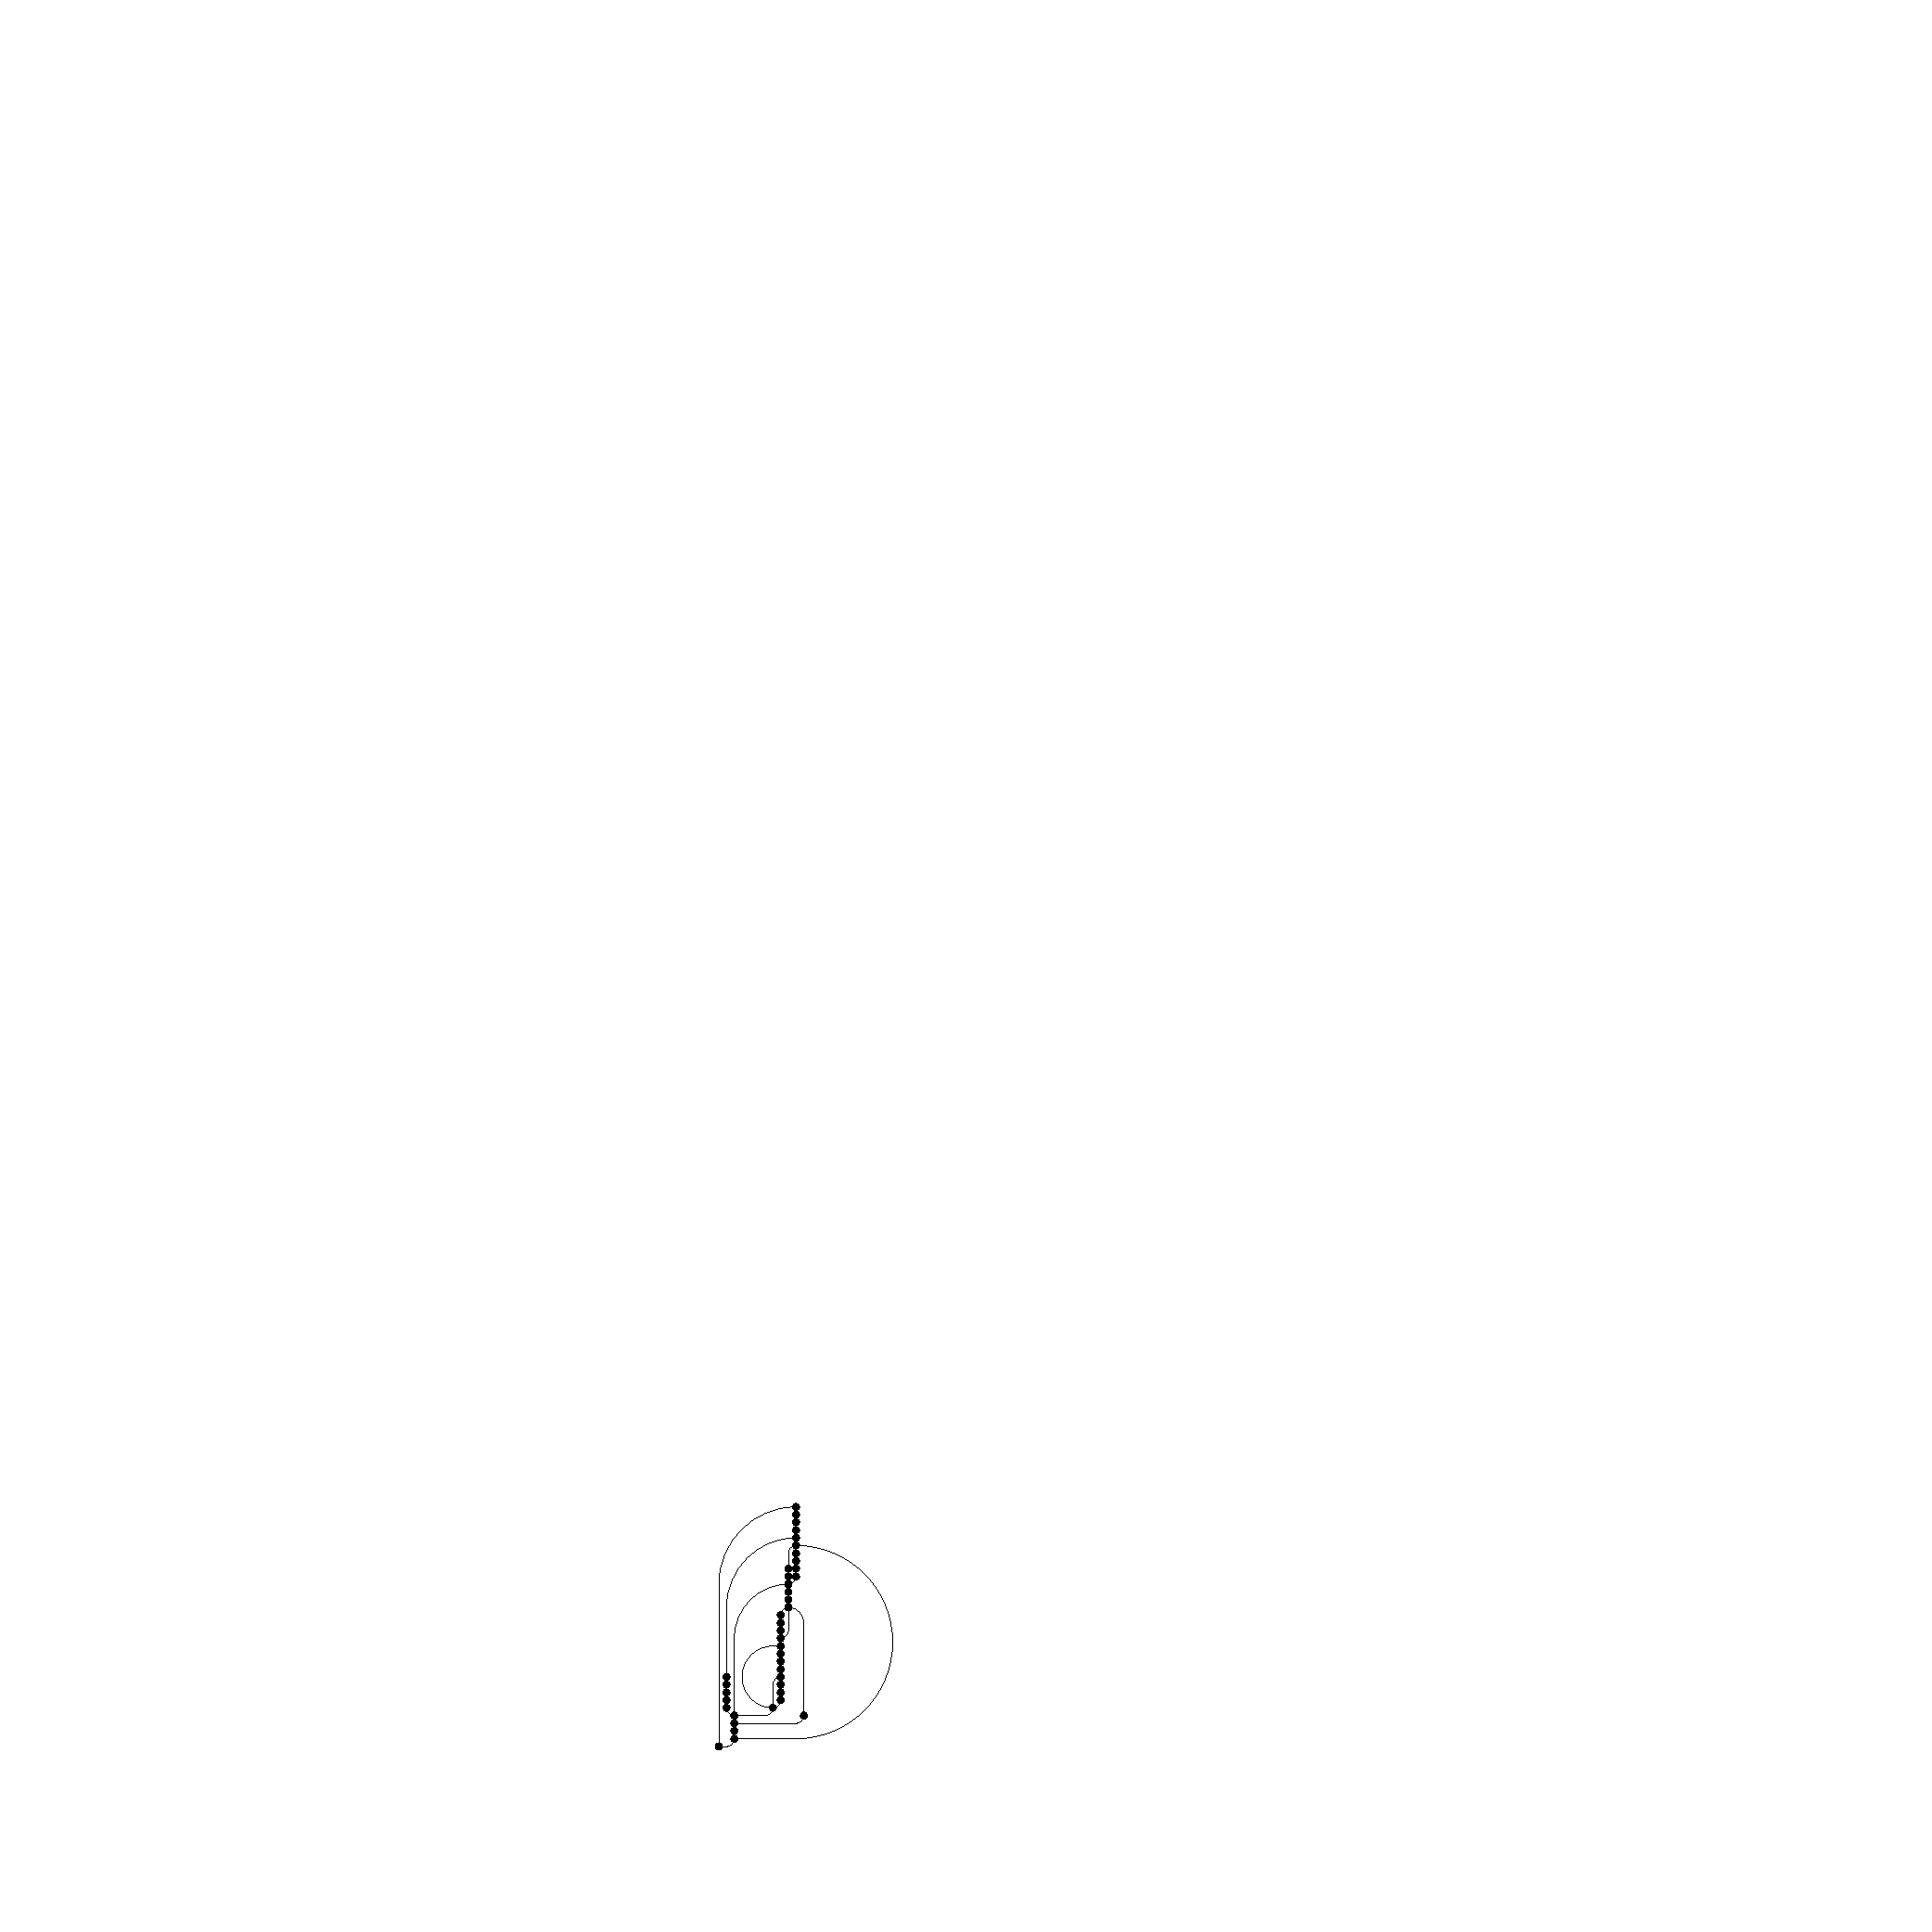
\includegraphics{hugeGraph/isSmaller}
  \caption{ Korrektur der Steigung ausgesetzt}
  \label{fig:exampleAsmoothSimple}
\end{figure}
\end{frame}



\begin{frame}
  \frametitle{ Platzbedarf von G"~Kanten}

\begin{columns}[b]
\begin{column}{5cm}
\begin{figure}[h]
  \centering
  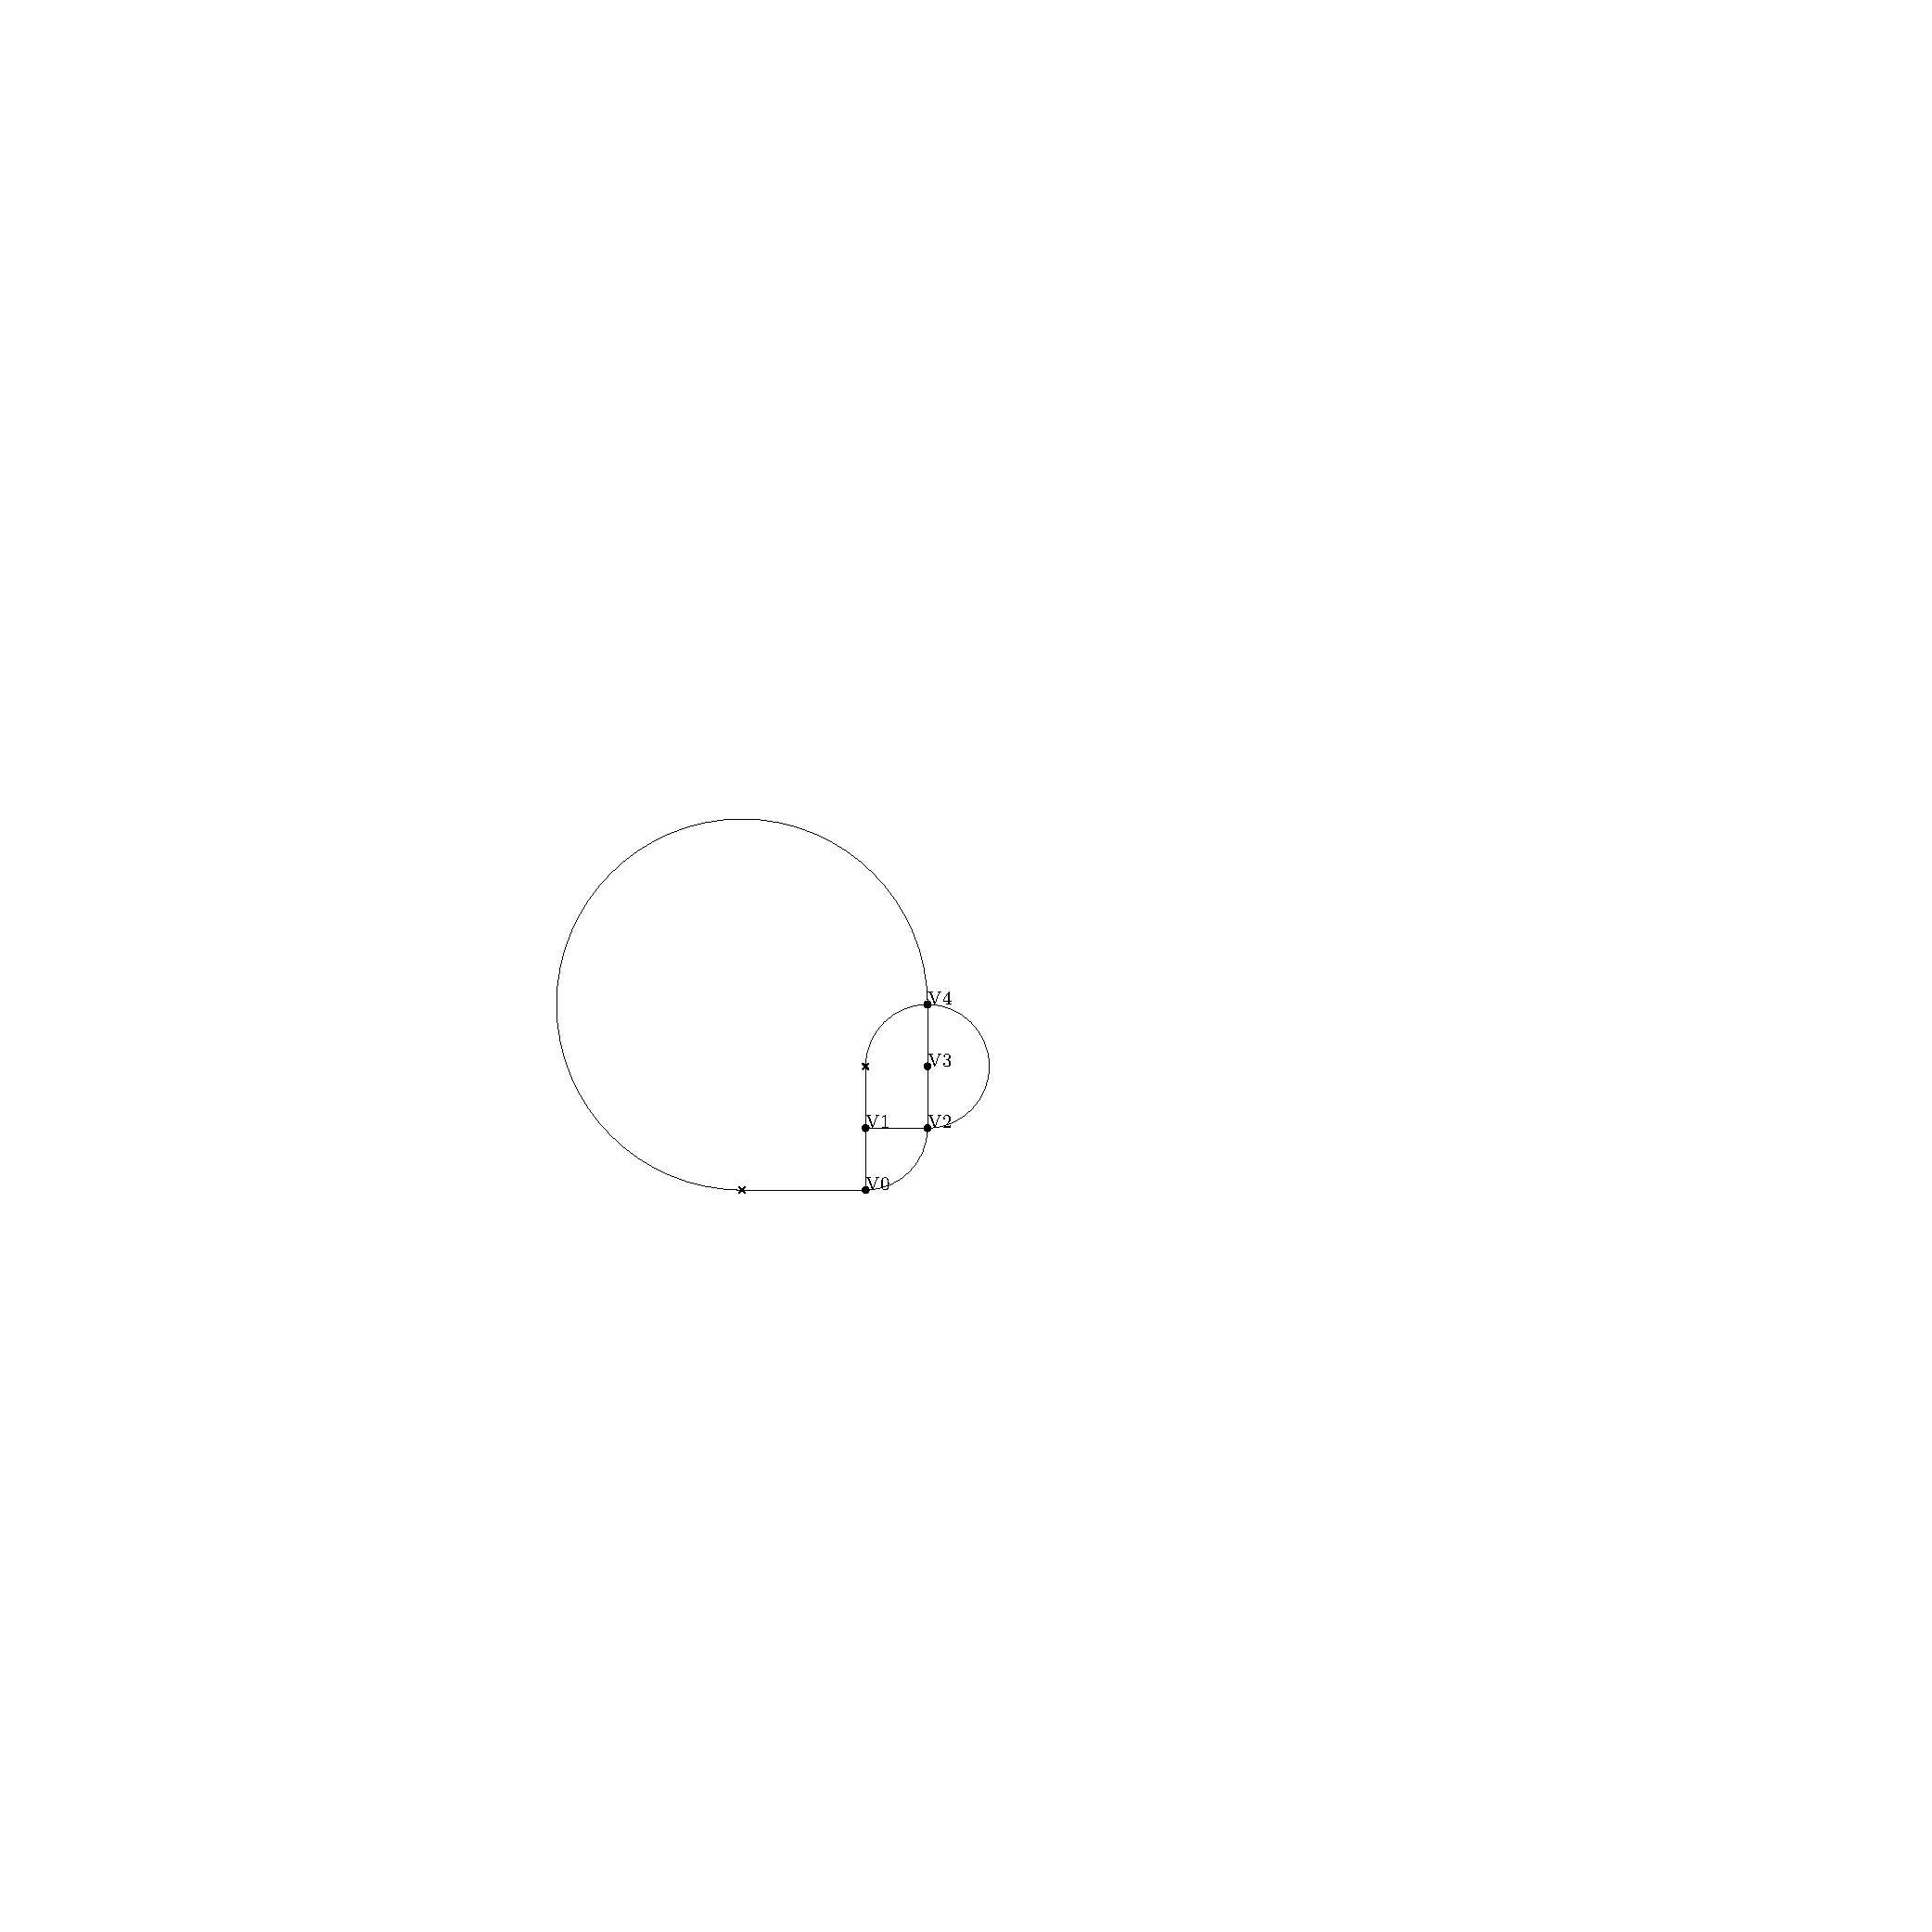
\includegraphics[scale=0.7]{exampleA/smooth}
  \caption{Mit Kante $\{0,4\}$ aus zwei Segmenten.}
  \label{fig:exampleAsmoothSimple}
\end{figure}
\end{column}
\begin{column}{5cm}
\begin{figure}[h]
  \centering
  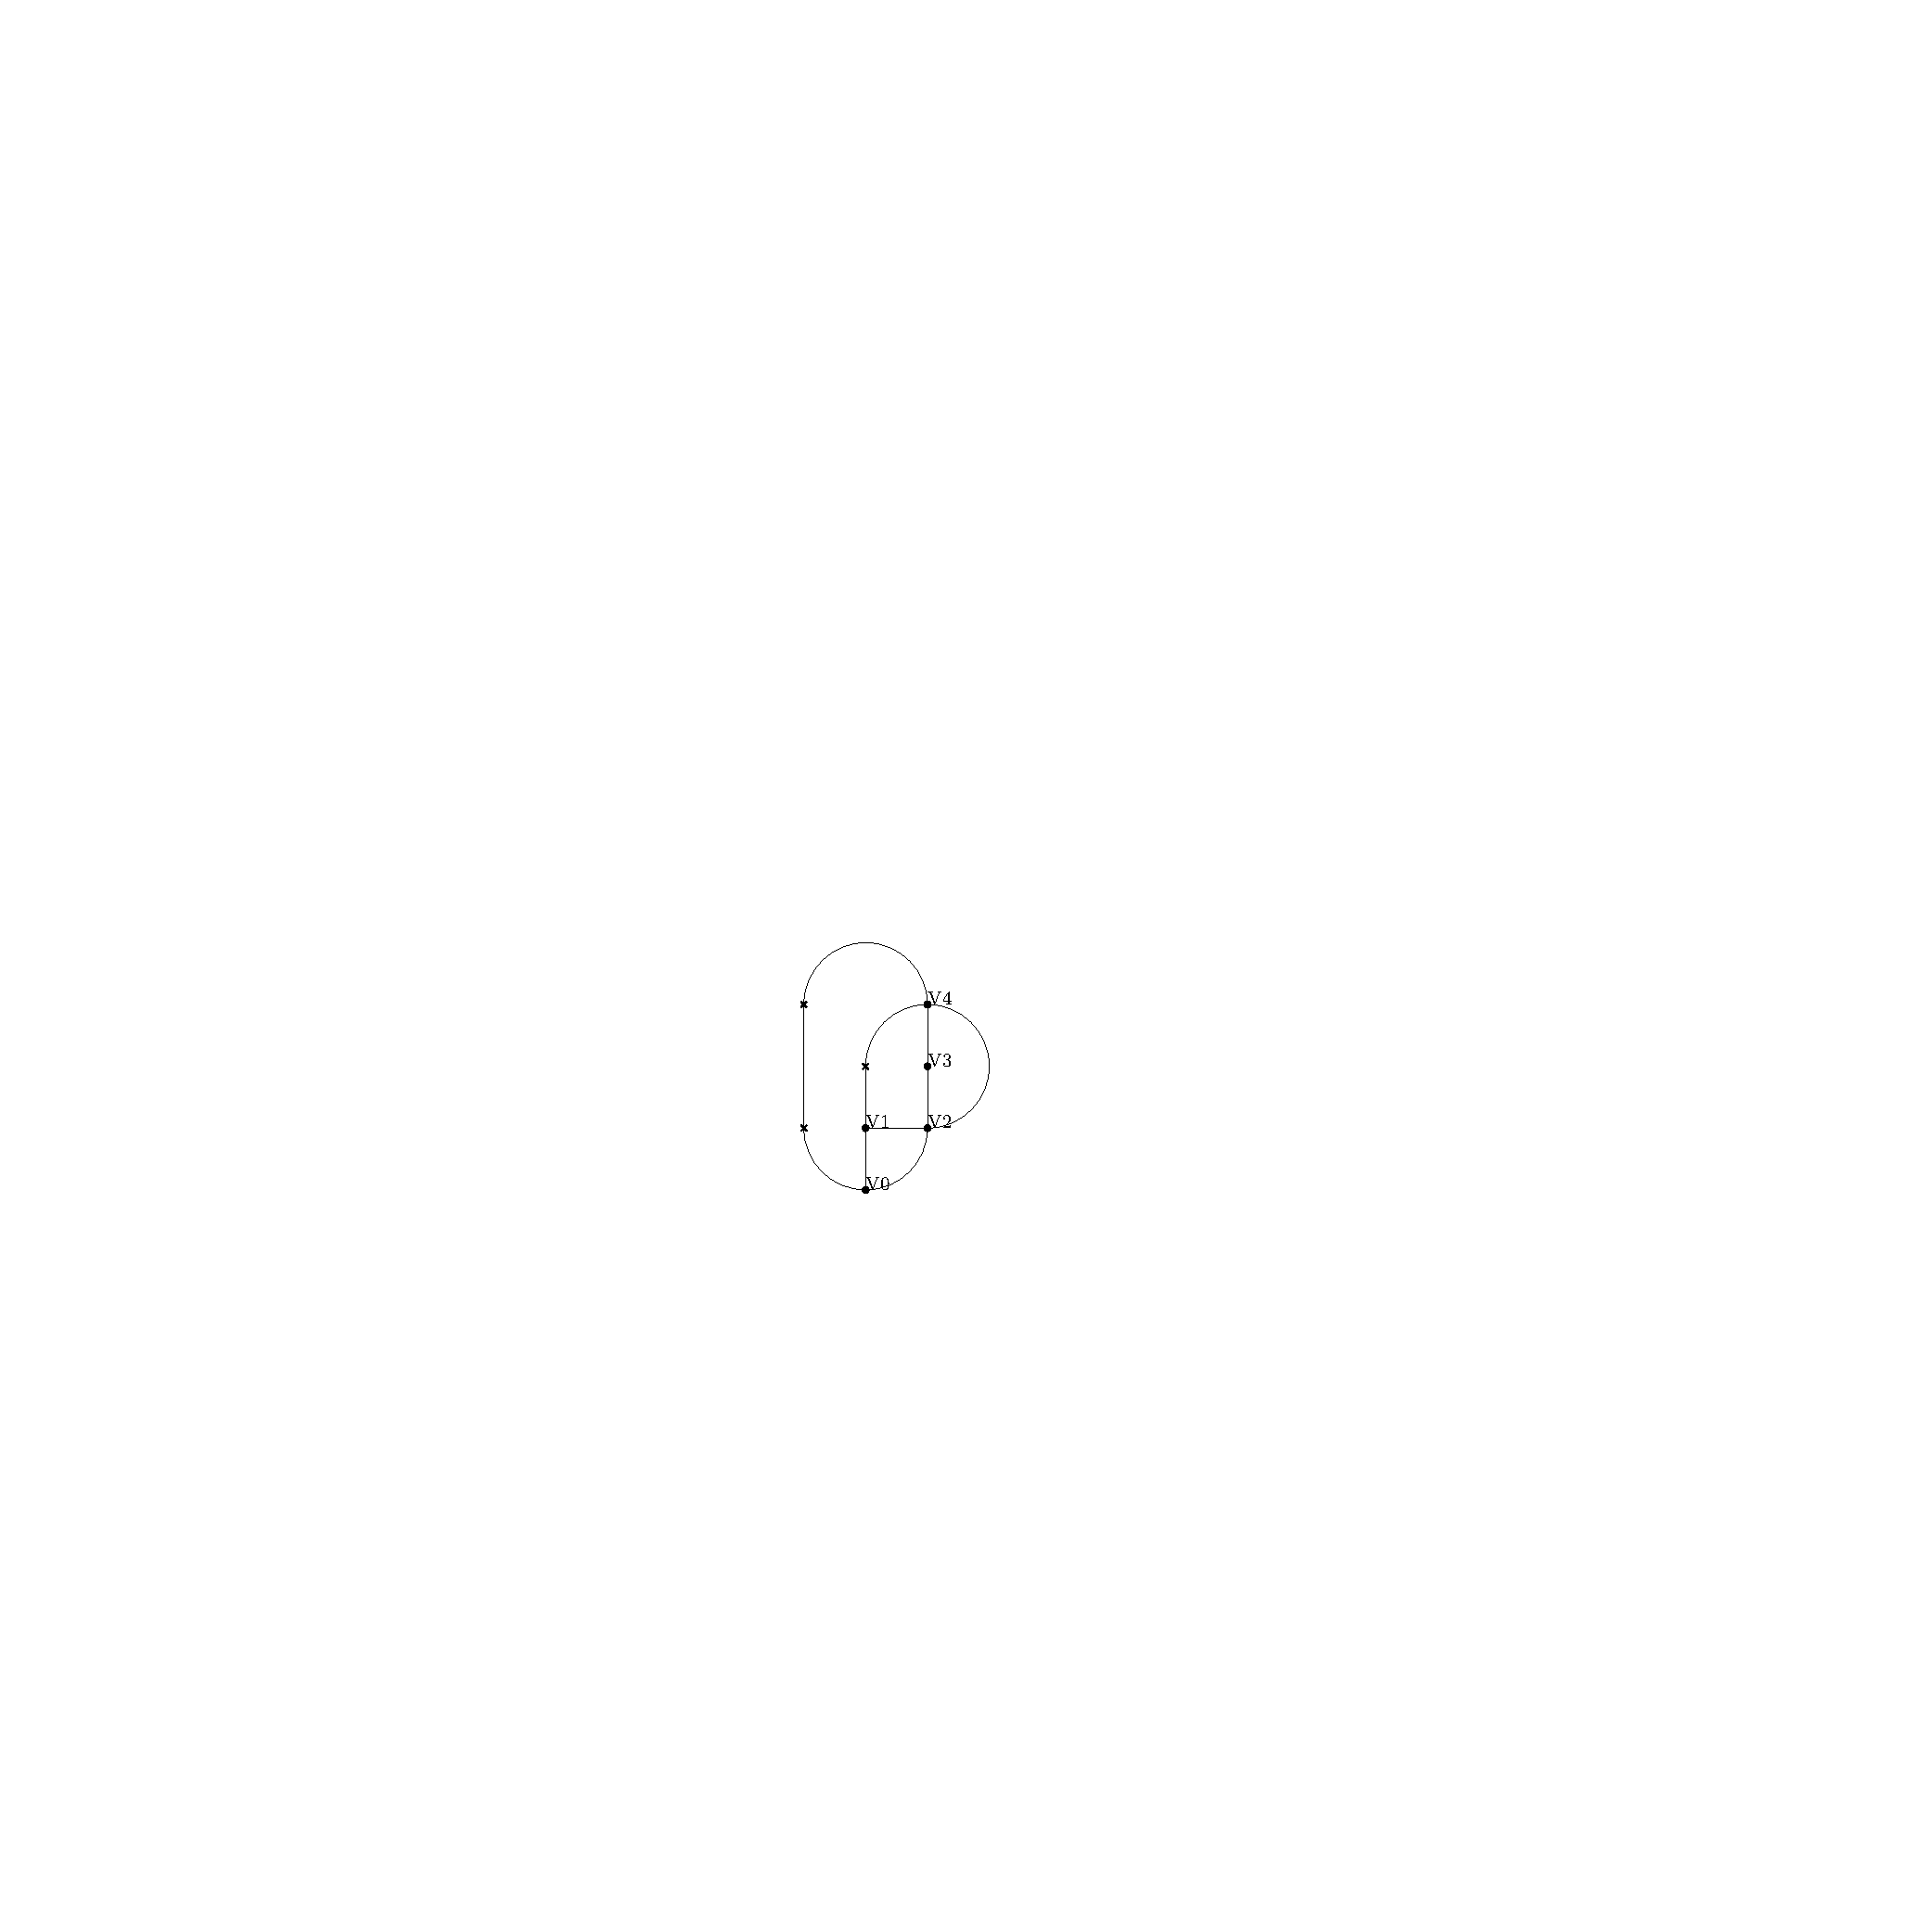
\includegraphics[scale=0.7]{exampleA/smoothComplex}
  \caption{Mit Kante $\{0,4\}$ aus drei Segmenten.}
  \label{fig:exampleAsmoothComplex}
\end{figure}
\end{column}
\end{columns}
\end{frame}


\begin{frame}
  \frametitle{Bewertungskriterien für glatt"=orthogonale Zeichnungen}
  \begin{itemize}[<+->]
    \item Fläche in Gittereinheiten
    \item Fläche in Abhängigkeit der Anzahl Knoten
    \item Anzahl Segmente in der Zeichnung
  \end{itemize}
\end{frame}

\begin{frame}
  \frametitle{Die Testgraphen}
  \begin{itemize}[<+->]
    \item 844 Rome-Graphen
    \item Oft zwischen 11 und 20 Knoten, durchschnittlich 18,2
    \item Bis zu 51 Knoten
    \item Nur 4-planar und zweifach zusammenhängend
  \end{itemize}
\end{frame}


\begin{frame}
\begin{figure}[h]
  \centering
  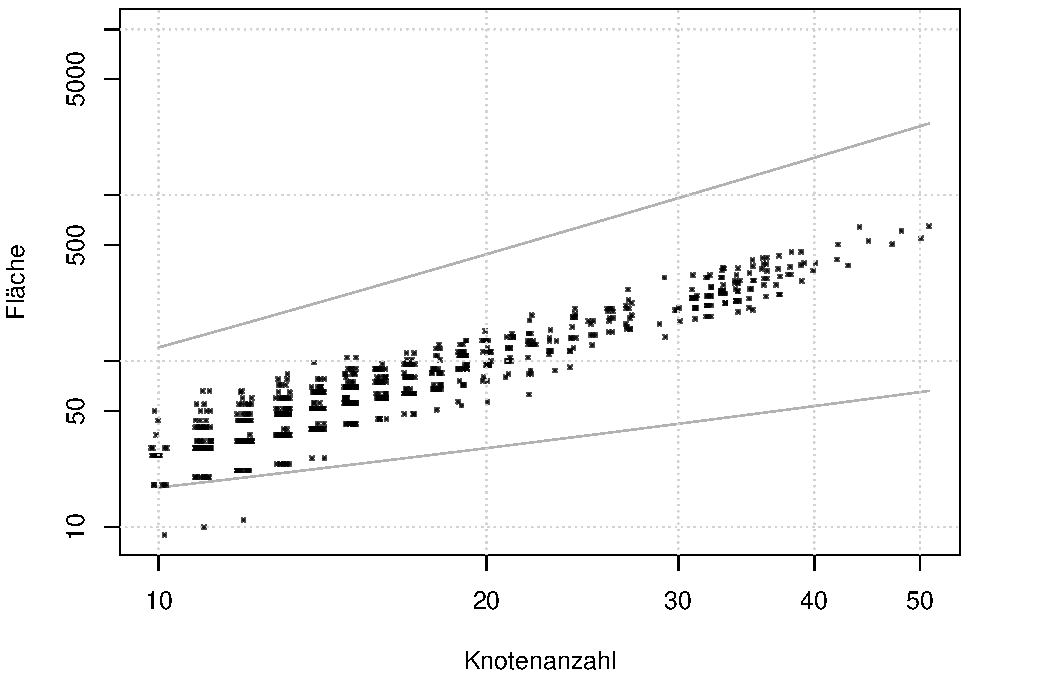
\includegraphics[width=.9\textwidth]{plots/area_orthogonal}
  \caption{OC$_3$-Zeichnungen ohne Kompression}
  \label{fig:ortho-compress}
\end{figure}
\end{frame}

\begin{frame}
\begin{figure}[h]
  \centering
  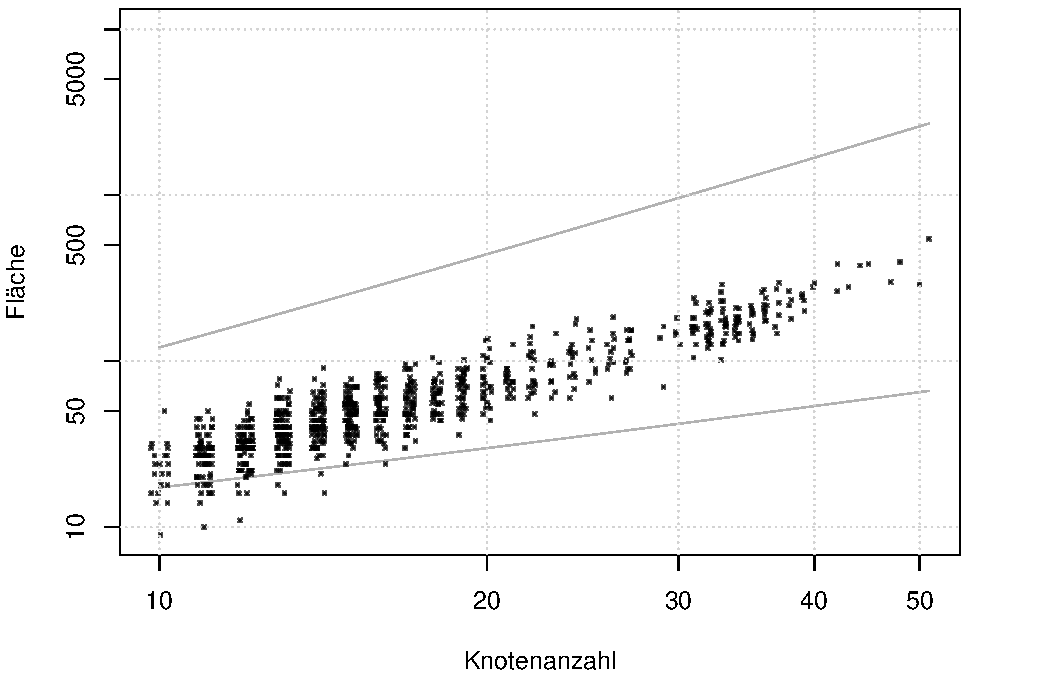
\includegraphics[width=.9\textwidth]{plots/area_orthogonal_compressed}
  \caption{OC$_3$-Zeichnungen nach Kompression, ohne Stufen}
  \label{fig:ortho-compress}
\end{figure}
\end{frame}

\begin{frame}
\begin{figure}[h]
  \centering
  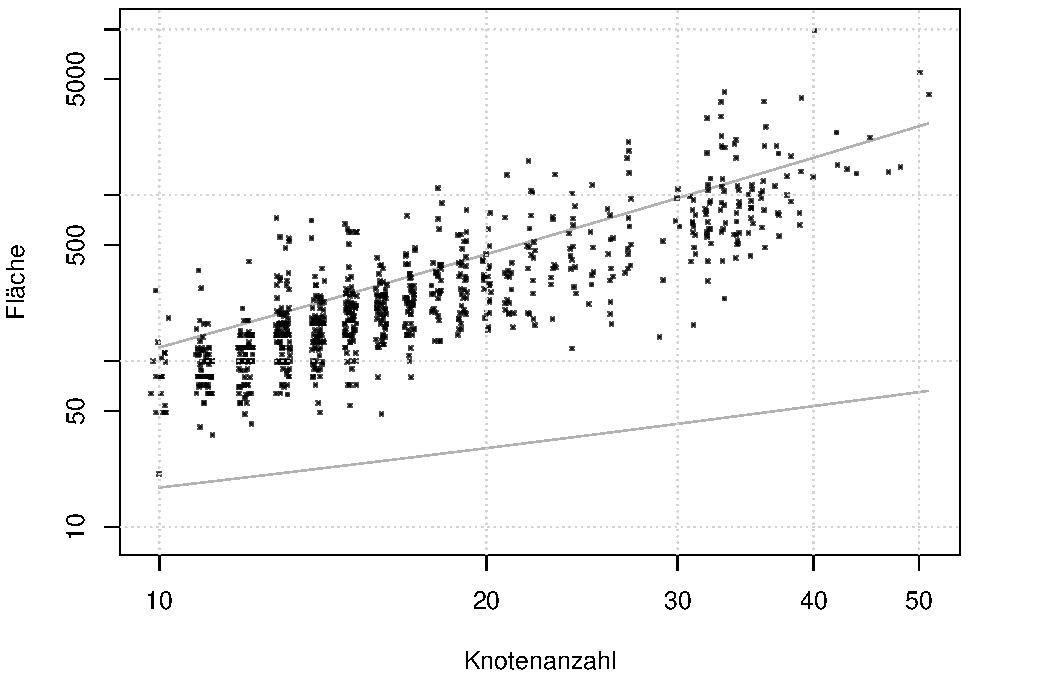
\includegraphics[width=.9\textwidth]{plots/area_smooth}
  \caption{SC$_2$-Zeichnungen, Steigung aller L"~Kanten berichtigt}
  \label{fig:smooth-noOpti}
\end{figure}
\end{frame}

\begin{frame}
\begin{figure}[h]
  \centering
  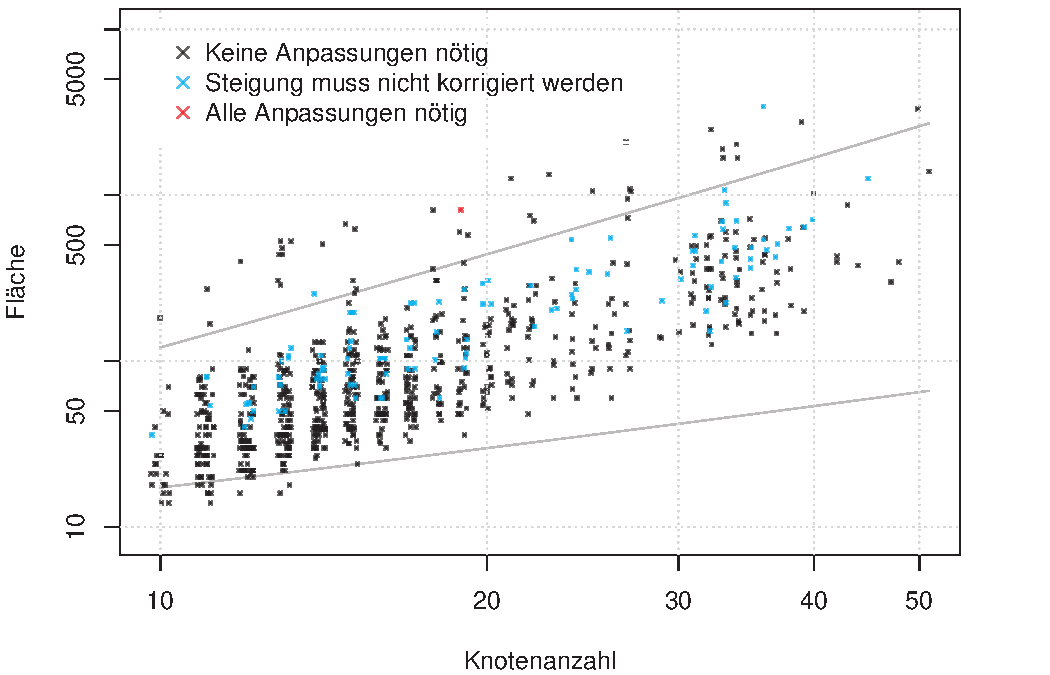
\includegraphics[width=.9\textwidth]{plots/area_smooth_bst}
  \caption{SC$_2$-Zeichnungen, Steigung L"~Kanten bei Bedarf berichtigt}
  \label{fig:smooth-opti}
\end{figure}
\end{frame}

\begin{frame}
\begin{figure}[h]
  \centering
  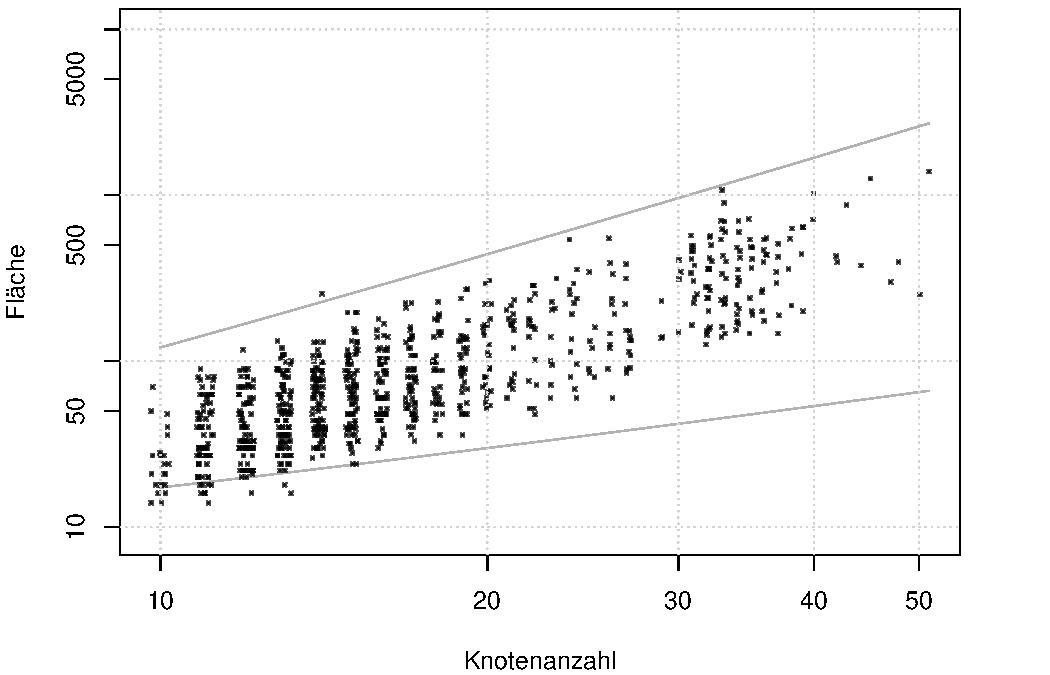
\includegraphics[width=.9\textwidth]{plots/area_smooth_noG}
  \caption{SC$_2$-Zeichnungen, ohne G"~Kanten}
  \label{fig:smooth-noG}
\end{figure}
\end{frame}

%\begin{frame}
%\begin{figure}[h]
%  \centering
%  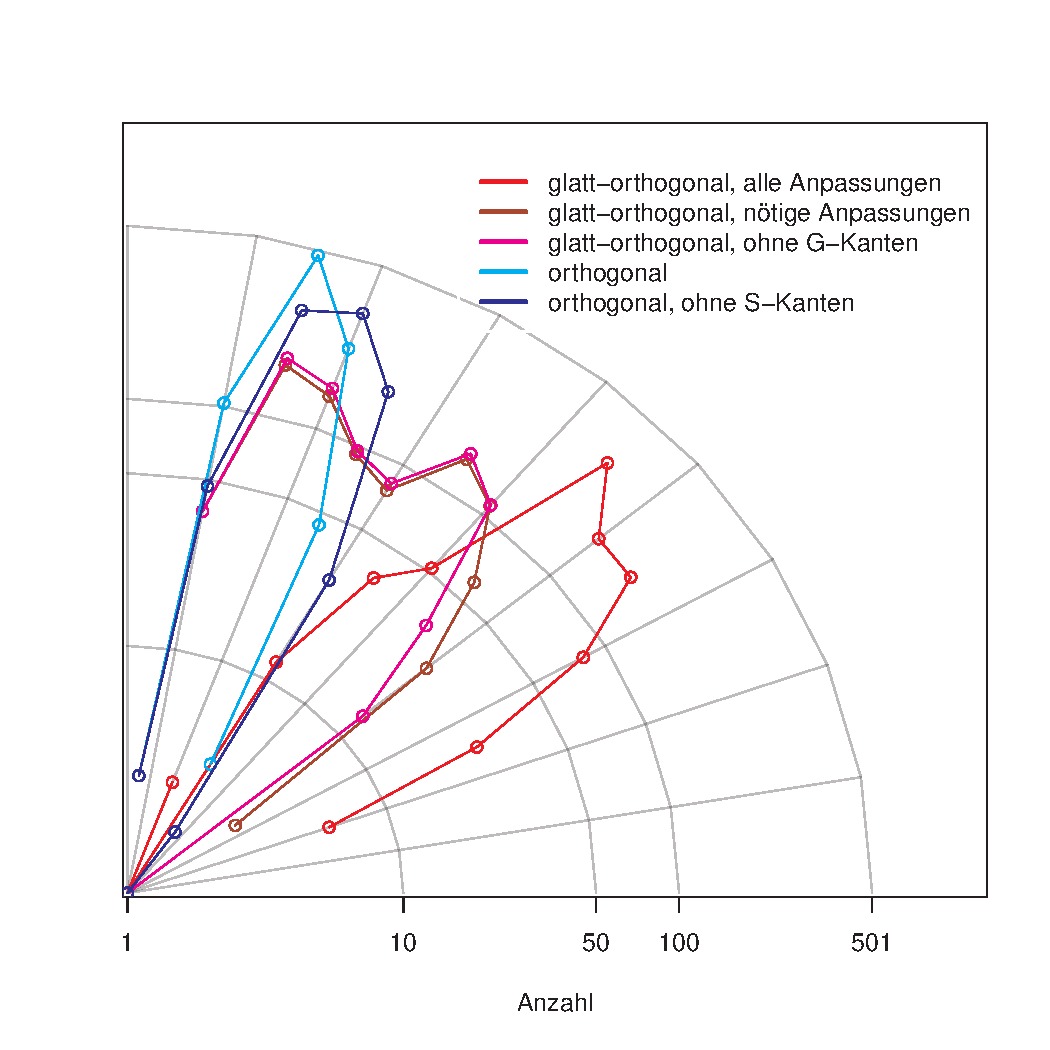
\includegraphics[width=.6\textwidth]{plots/angles_comparison}
%  \caption{Verteilung der Seitenverhältnisse der Zeichnungen.}
%  \label{fig:angleComparison}
%\end{figure}
%\end{frame}

%\begin{frame}
%\begin{figure}[h]
%  \centering
%  {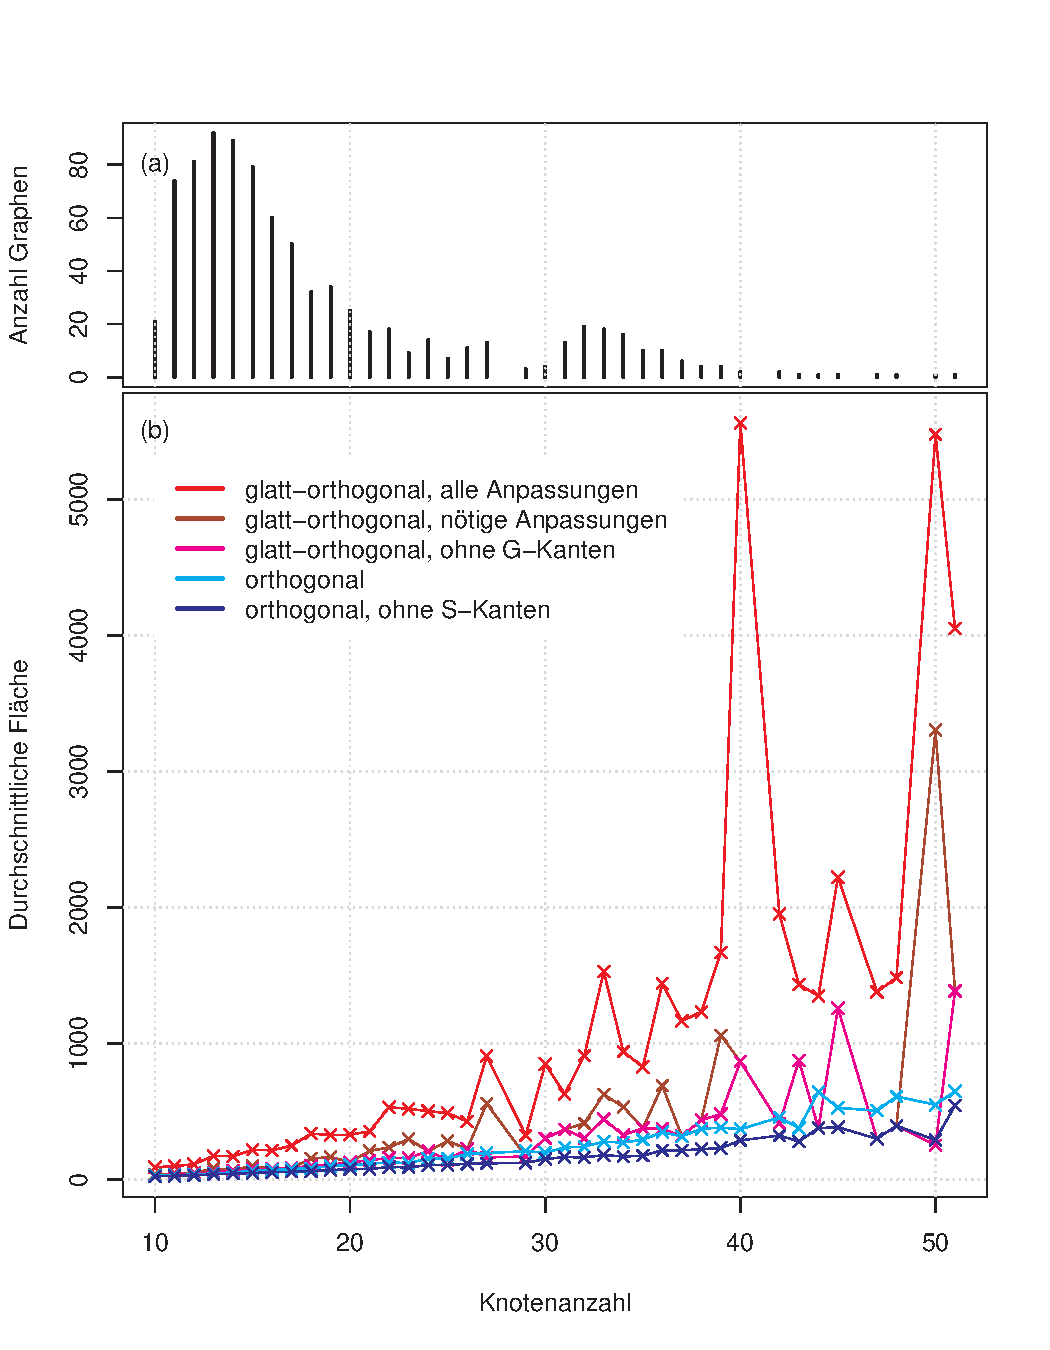
\includegraphics[height=\textheight]{plots/area_comparison}}
%  \caption{Vergleich des durchschnittlichen Flächenbedarfs in Gitterquadraten der verschiedenen Algorithmen nach Anzahl Knoten im Graphen (a) sowie  Verteilung der Anzahl Knoten in den Graphen (b). Zum Vergleich: Eine DIN-A4-Seite von handelsüblichem kariertem Papier hat rund 2400 Gitterquadrate.}
%  \label{fig:areaComparisonAndGraphSizes}
%\end{figure}
%\end{frame}




\begin{frame}
  \frametitle{Ausblick}
  \begin{itemize}[<+->]
    \item Bessere Laufzeit bei Kollisionsprüfung
    \item Noch platzsparendere Zeichnungen
    \item Untersuchung allgemeinerer Graphen
      \begin{itemize}[<+->]
        \item Nicht planar
        \item nicht zweifach zusammenhängend
        \item nicht zusammenhängend
        \item höherer Grad als~4
        \item \dots
      \end{itemize}
    \item Anwendung: automatischer Liniennetzplan
  \end{itemize}
\end{frame}


\begin{frame}[shrink=30]
  \frametitle{Literatur}
  \bibliographystyle{mybabalpha-fl}
  \small\bibliography{mybib}
\end{frame}



\end{document}
